\chapter[Visão do Produto]{Visão do Produto}

\section{Visão Estrutural}

\subsubsection{Estrutura}
No desenho da estrutura do Robô priorizou-se: a identificação da criança com o equipamento e a sua segurança.
O produto foi confeccionado para minimizar os riscos a integridade física da criança, foi feito com design “macio”,
não apresentando pontas ou qualquer componente que venha a amplificar um possível dano causado por contato.

No que diz respeito à cor o estudo de \citeonline{pagnan:2009} afirma que a cor exerce uma ação tríplice: a de impressionar
a de expressar e a de construir, portanto o aparelho deve apresentar coloração atrativa para a criança, o trabalho também
faz uma relação entre as cores e seus respectivos significados psicológicos e simbólicos, para os propósitos do trabalho
selecionamos as cores:

\begin{itemize}
    \item \textbf{Azul}: Exerce apelo intelectual, simbolizando a inteligência e raciocínio;
    \item \textbf{Vermelho}: Estimulante e dinâmica é a cor preferida da criança.
\end{itemize}

O robô foi construído na forma de um carrinho, por ser um elemento a qual a criança já está acostumada, esse critério
é importante uma vez que a não aceitação visual da criança pelo produto, pode levar a bloqueios no aprendizado na hora
de utilizar o produto. Alguns elementos como iluminação a LED e desenhos foram introduzidos na estrutura física de modo
a tornar o carrinho ainda mais atrativo para a criança.

Quanto ao material utilizado para confeccionar a estrutura os critérios utilizado para seleção foram: Segurança da
criança, propriedades mecânicas e proteção dos equipamentos eletrônicos. Assim como no design, deve se minimizar os
riscos a criança também na seleção dos materiais, o material precisa absolver bem os choques e não ser muito pesado
de modo a não causar muito dano em um possível impacto. Também não pode apresentar nenhum nível de toxicidade.

Do ponto de vista da integridade estrutural o carrinho será utilizado em um ambiente razoavelmente seguro, os riscos
de impactos são mínimos, uma vez que a velocidade que o carrinho atinge é razoavelmente baixa. Portanto as situações que
ameaçam a integridade estrutural do carrinho são a queda e o sobrepeso.

\subsubsection{Materiais}

Tomando como base os requisitos descritos acima, a escolha mais indicada de material seria os polímeros, porem levando em
conta o histórico de desenvolvimento de robôs desse porte, foi consideramos também o alumínio. As propriedades de ambos os materiais
satisfazem os requisitos, porem o polietileno apresenta a vantagem de ser mais macio e apresentar menos risco as crianças.

Em um primeiro momento do trabalho foi tomada a decisão de produzir o carrinho utilizando polietileno de alta densidade, a
forma das peças seria produzido por injeção, esse método é bastante atrativo principalmente pelo preço de compra do material
para esse processo. Porém não se encontrou na faculdade o maquinário necessário para trabalhar dessa maneira, a alternativa foi
procurar comprar chapas de polietileno e realizar operações de furos e cortes para colocar o material na forma desejada, novamente
esbarramos no problema da falta de equipamento além do enorme preço do material, a solução para todos esses problemas e a
definitiva foi procurar uma alternativa mais barata e fácil de trabalhar do que o polietileno decidiu-se usar o MDF. O MDF
possui propriedades físicas bastante semelhantes ao polietileno e embora seja mais duro ele é macio o suficiente para essa aplicação.

\begin{figure}[H]
    \centering
    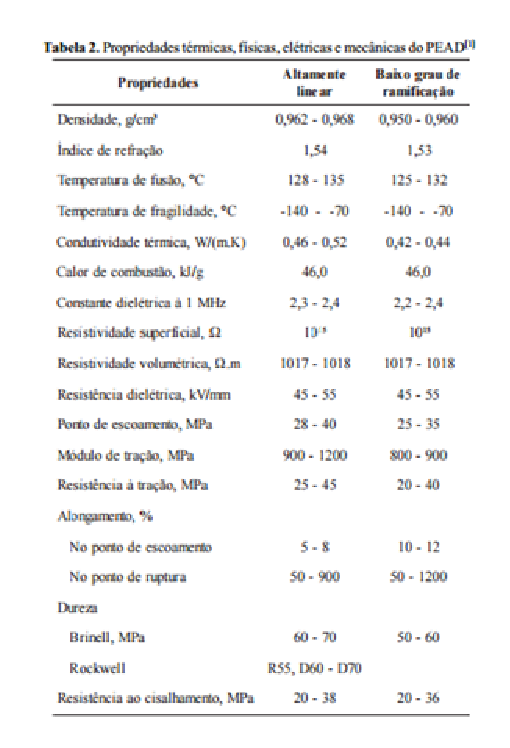
\includegraphics[width=0.5\textwidth]{figuras/pp_HDPE.eps}
    \caption{Propriedades do HDPE}
    \label{fig:pp_HDPE}
\end{figure}

\begin{figure}[H]
    \centering
    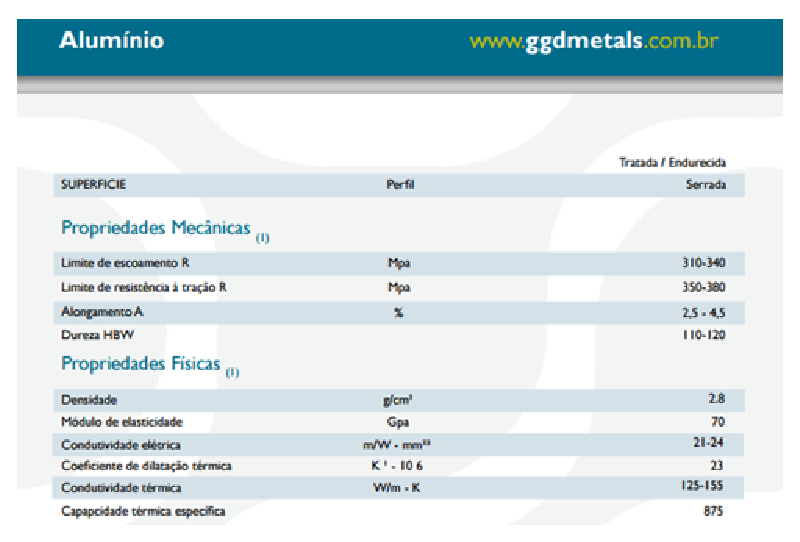
\includegraphics[width=0.8\textwidth]{figuras/pp_aluminio.eps}
    \caption{Propriedades do Alumínio CAST 7000}
    \label{fig:pp_aluminio}
\end{figure}


\begin{figure}[H]
    \centering
    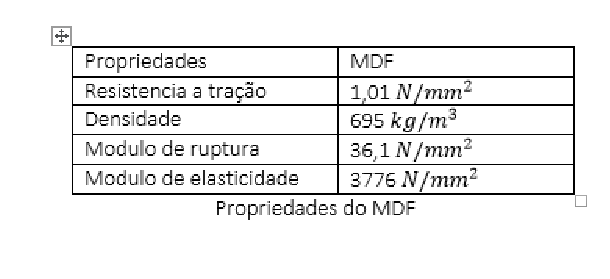
\includegraphics[width=0.5\textwidth]{figuras/pp_MDF.eps}
    \caption{Propriedades do MDF}
    \label{fig:pp_MDF}
\end{figure}

As propriedades do MDF listadas acima são propriedades medias, uma vez que dependendo de alterações sutis como o tipo de
tratamento elas mudam. A tabela acima foi montada com base na edição de número 125 da revista da madeira.

\subsubsection{Modelagem}

Para fazer a modelagem do carrinho utilizou-se o software CATIA V5-R16, a escolha deste software se justifica pelo fato do
conhecimento prévio das suas ferramentas pelos integrantes do grupo, todas as peças foram desenhadas no Part Design e unidas
no Assembly, nessa etapa também se coloca os materiais de cada componente. Base de movimentação:

\begin{figure}[H]
    \centering
    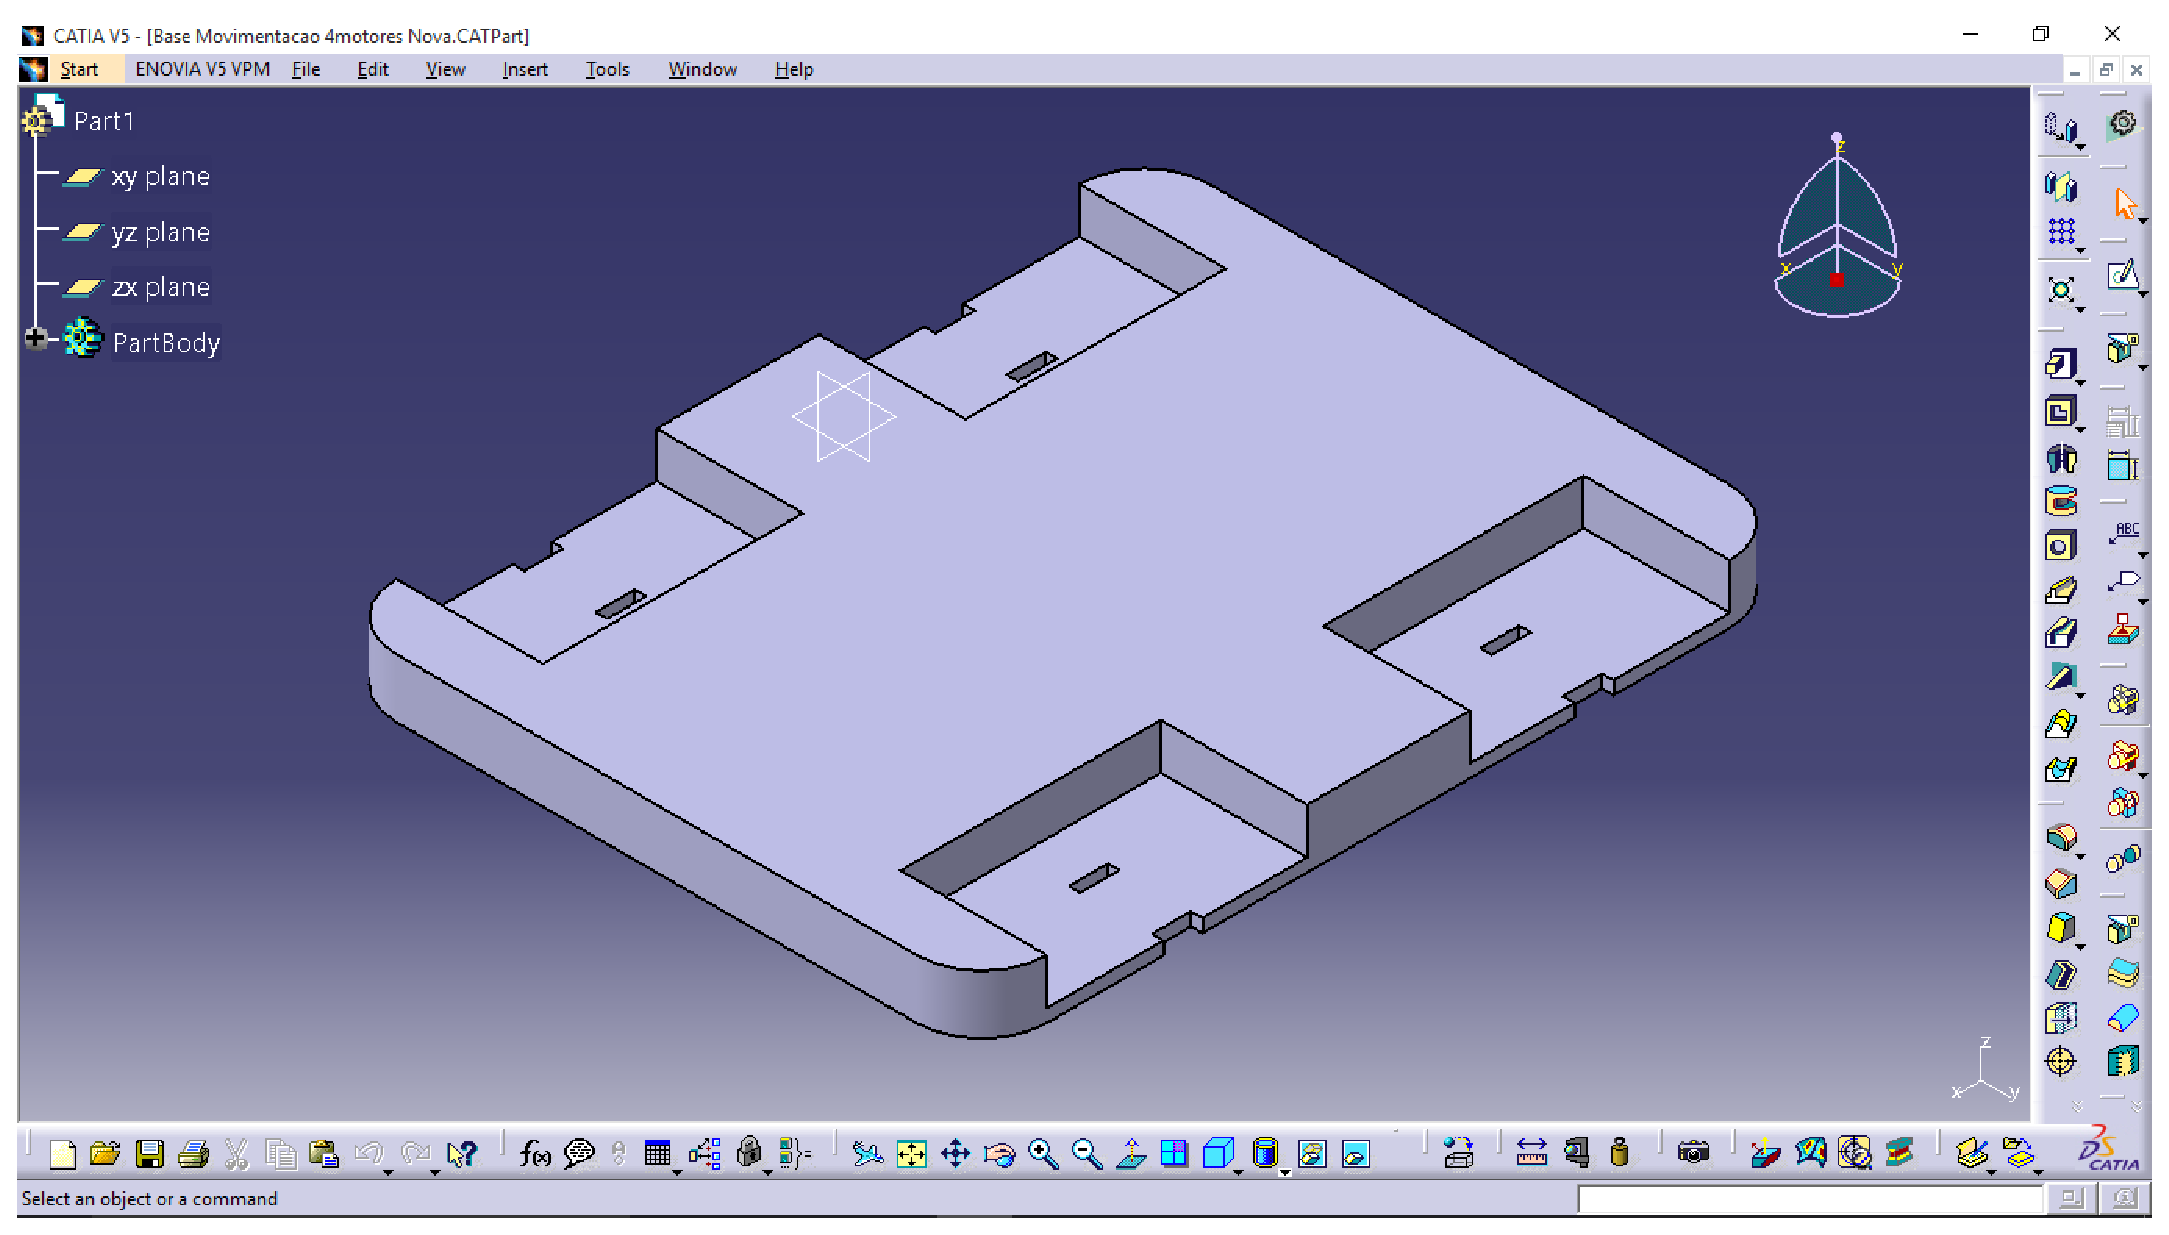
\includegraphics[width=0.7\textwidth]{figuras/base.eps}
    \caption{Base de Movimentação}
    \label{fig:base}
\end{figure}


\begin{figure}[H]
    \centering
    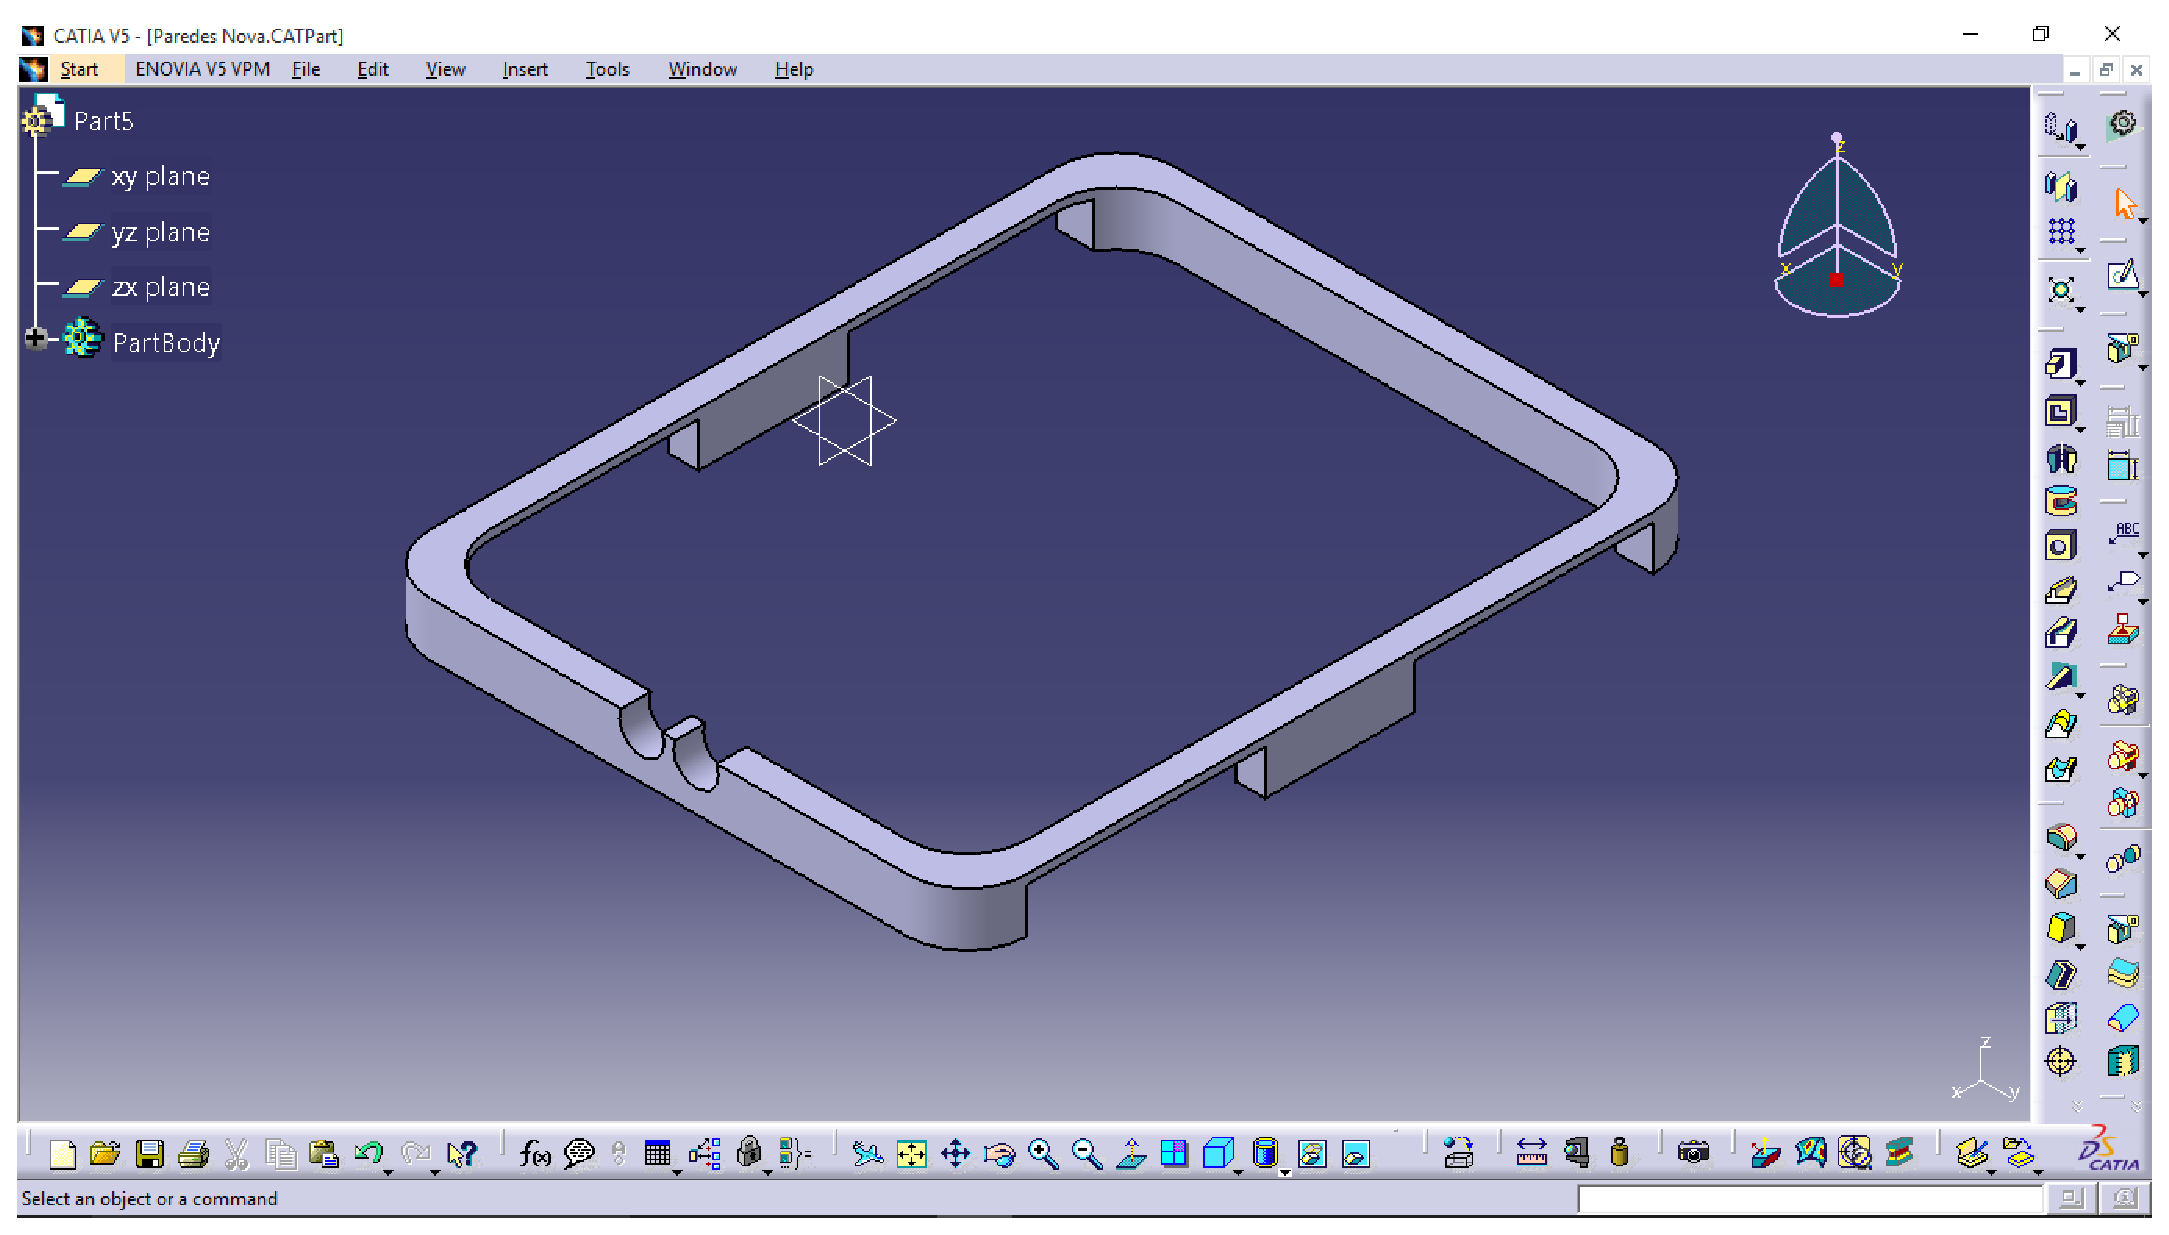
\includegraphics[width=0.7\textwidth]{figuras/inferior.eps}
    \caption{Parte Inferior}
    \label{fig:inferior}
\end{figure}


\begin{figure}[H]
    \centering
    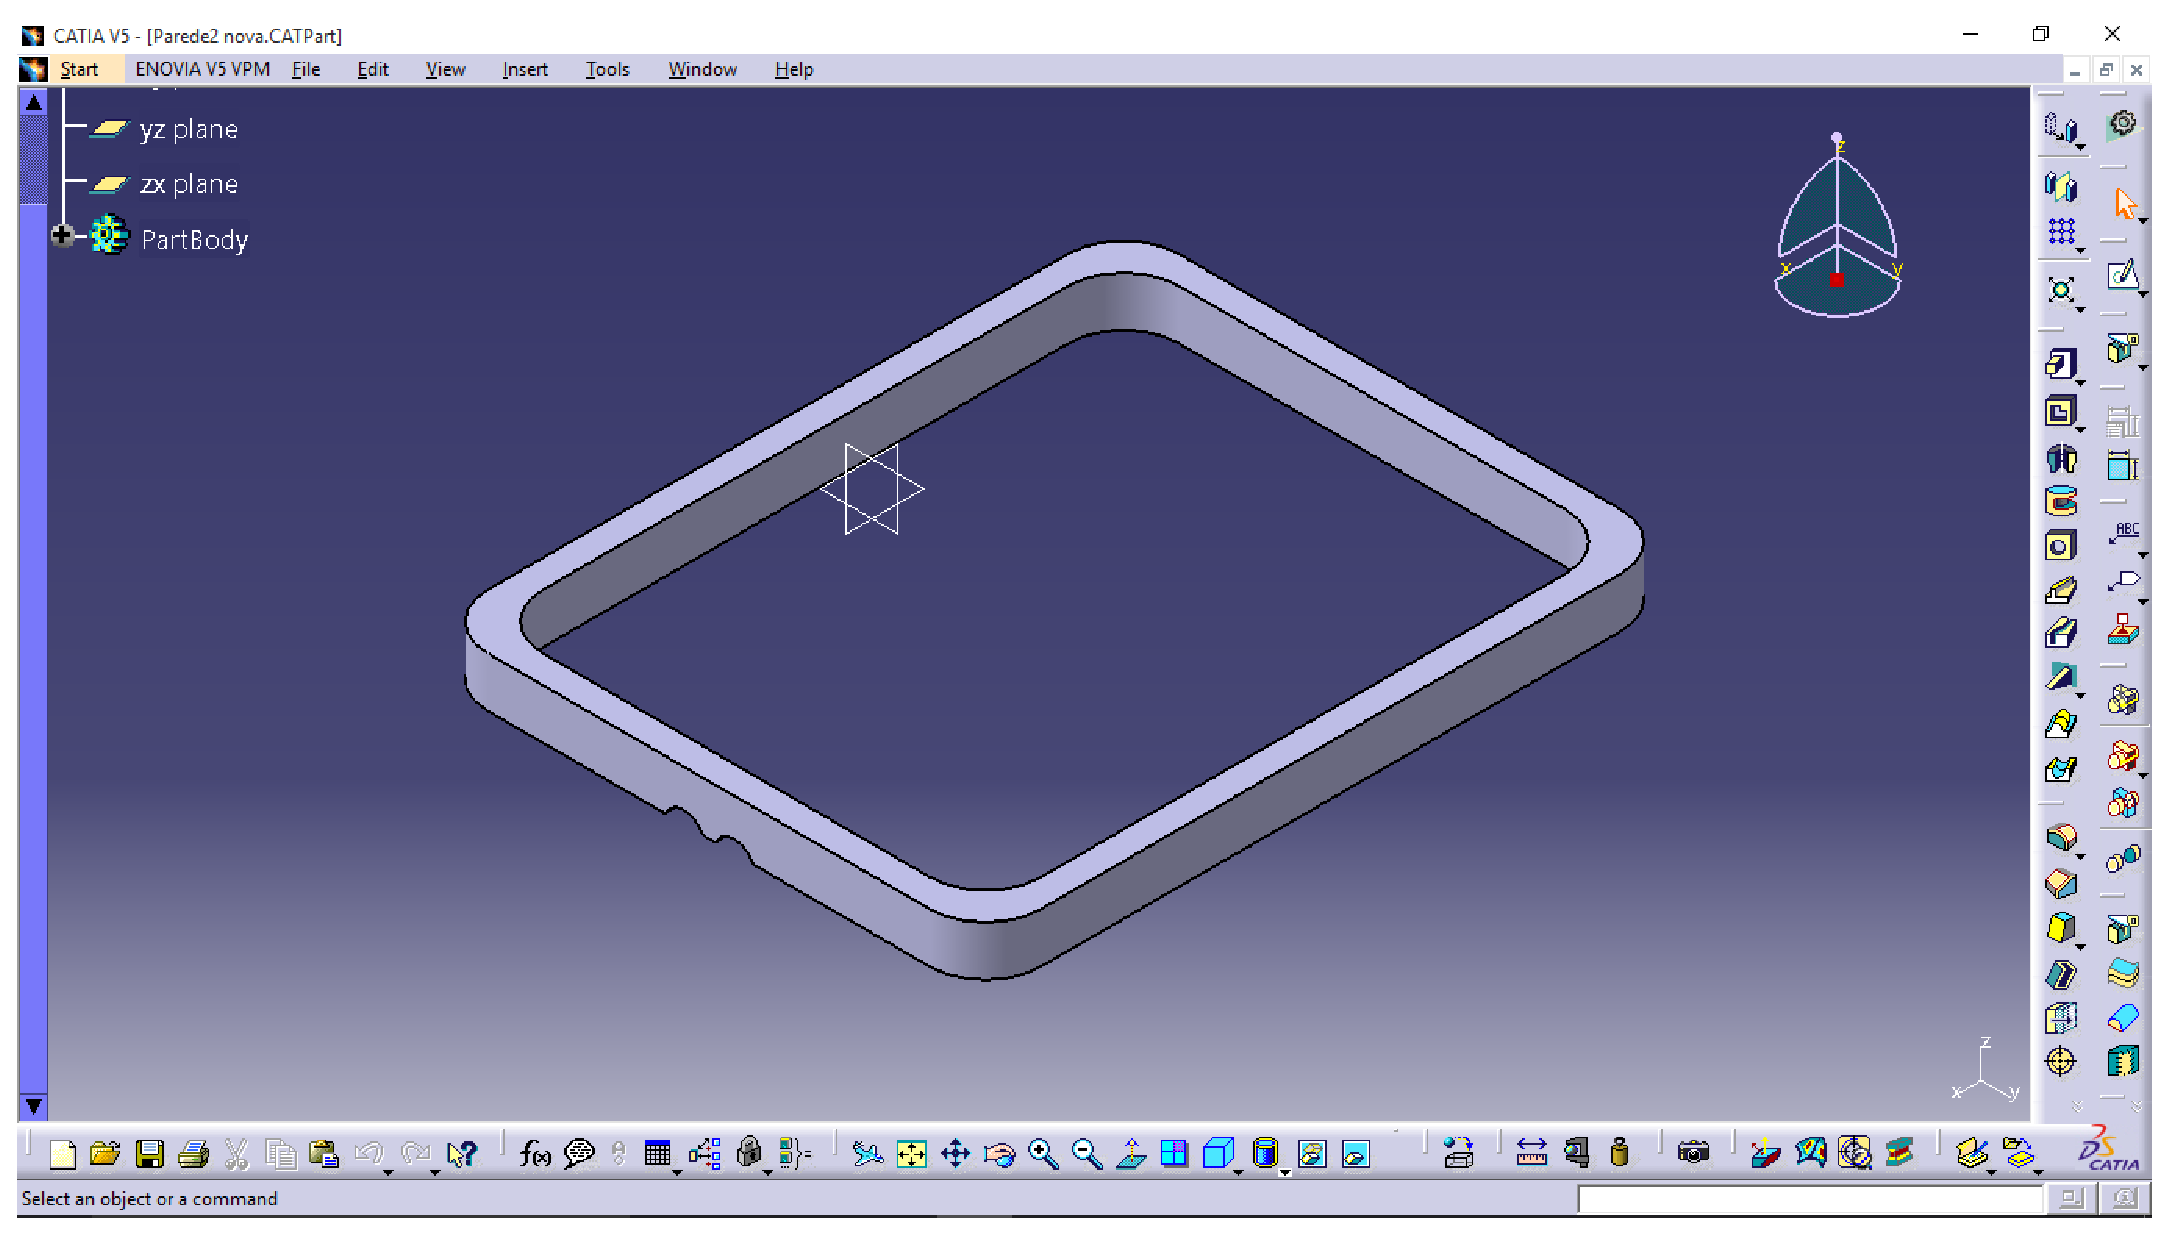
\includegraphics[width=0.7\textwidth]{figuras/superior.eps}
    \caption{Parte Superior}
    \label{fig:superior}
\end{figure}


\begin{figure}[H]
    \centering
    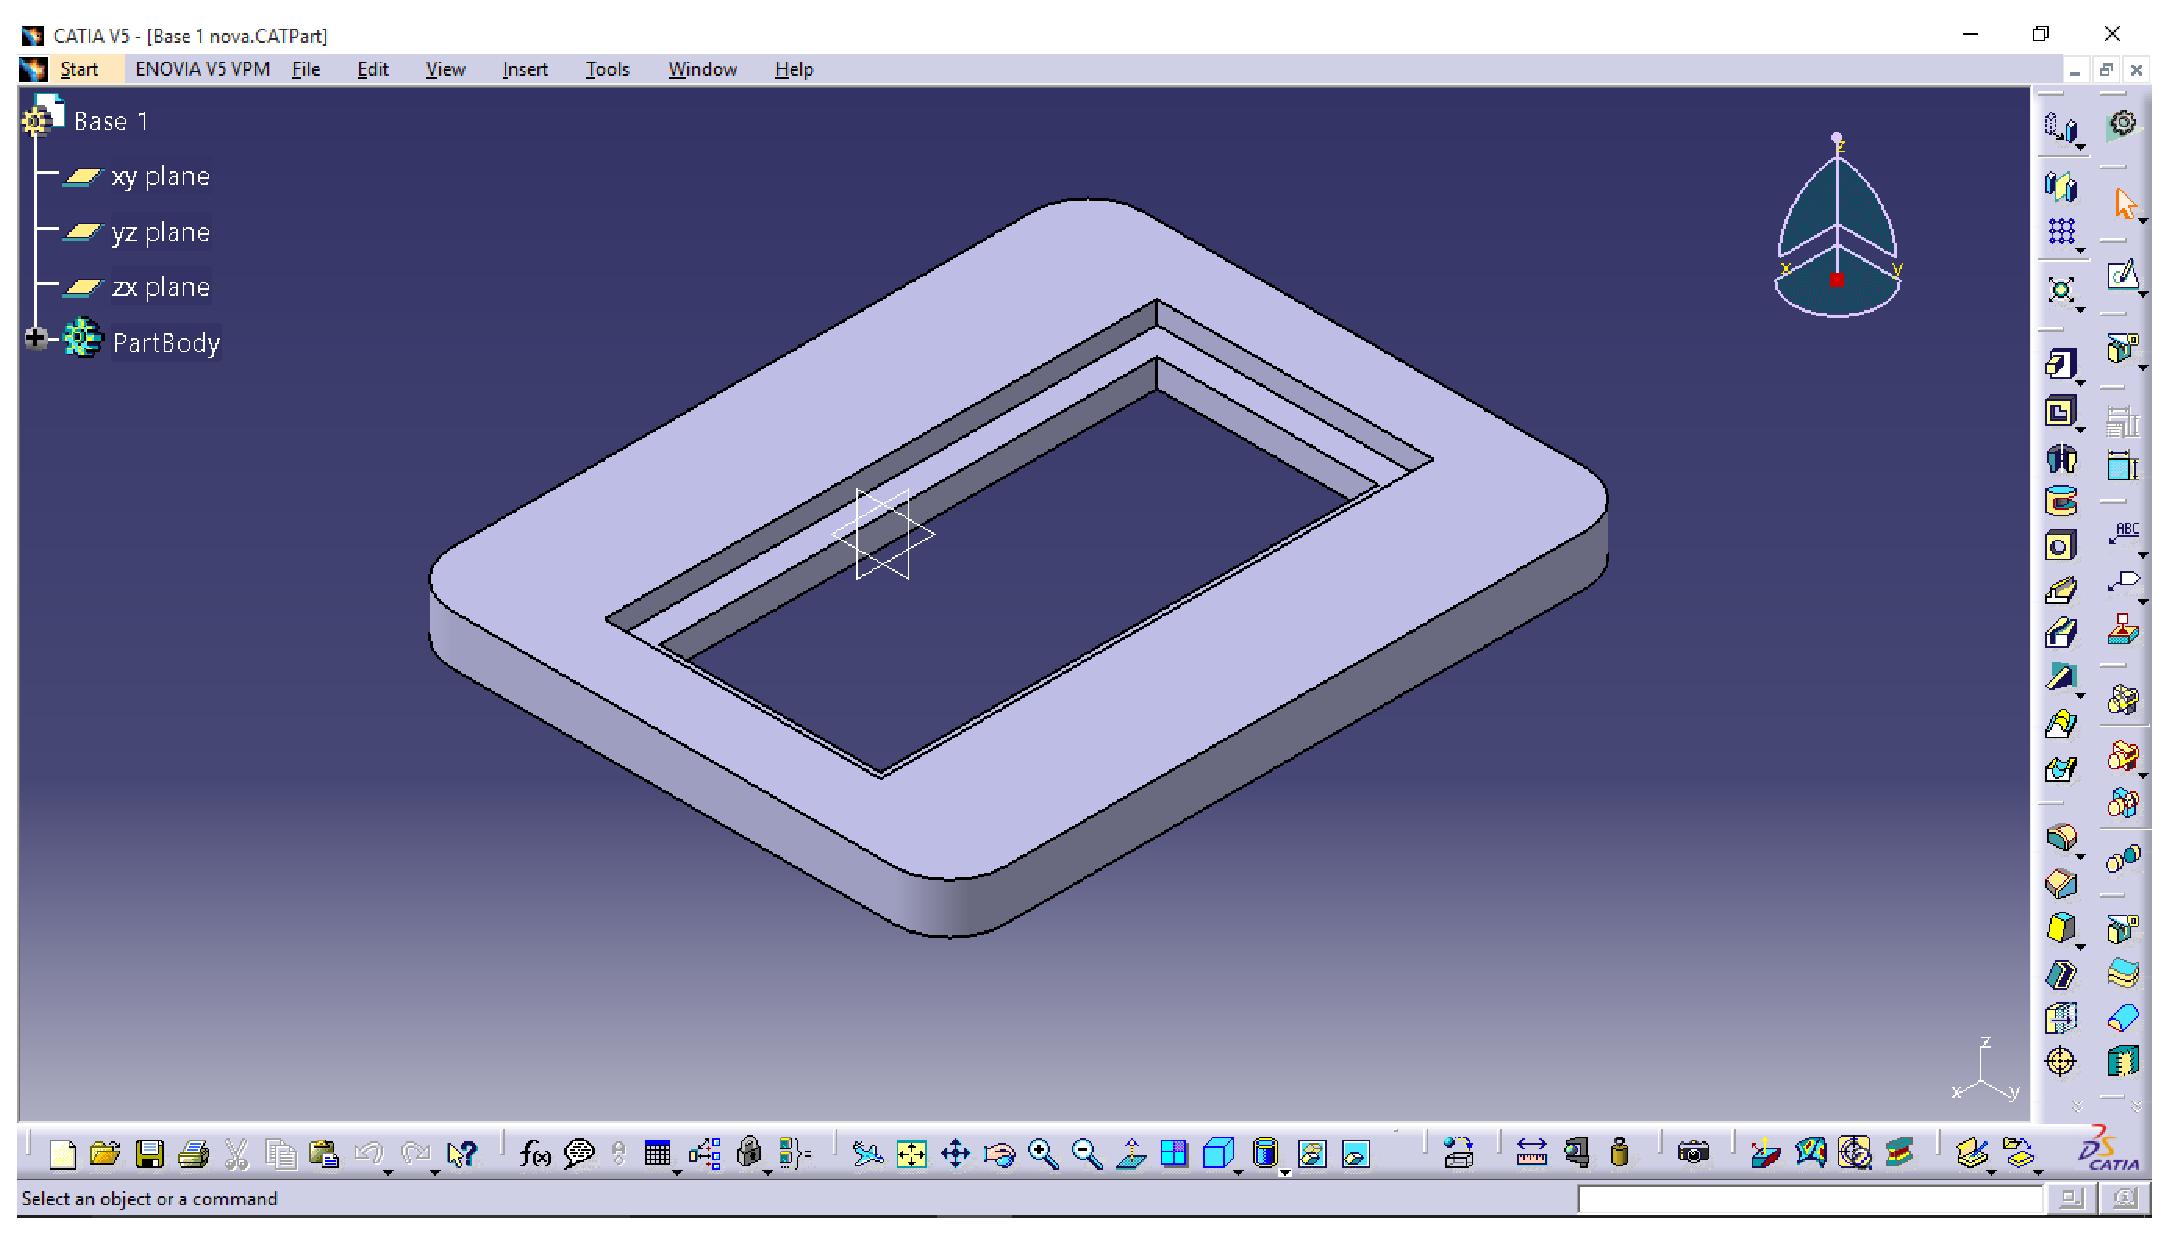
\includegraphics[width=0.7\textwidth]{figuras/cobertura.eps}
    \caption{Cobertura}
    \label{fig:cobertura}
\end{figure}


\begin{figure}[H]
    \centering
    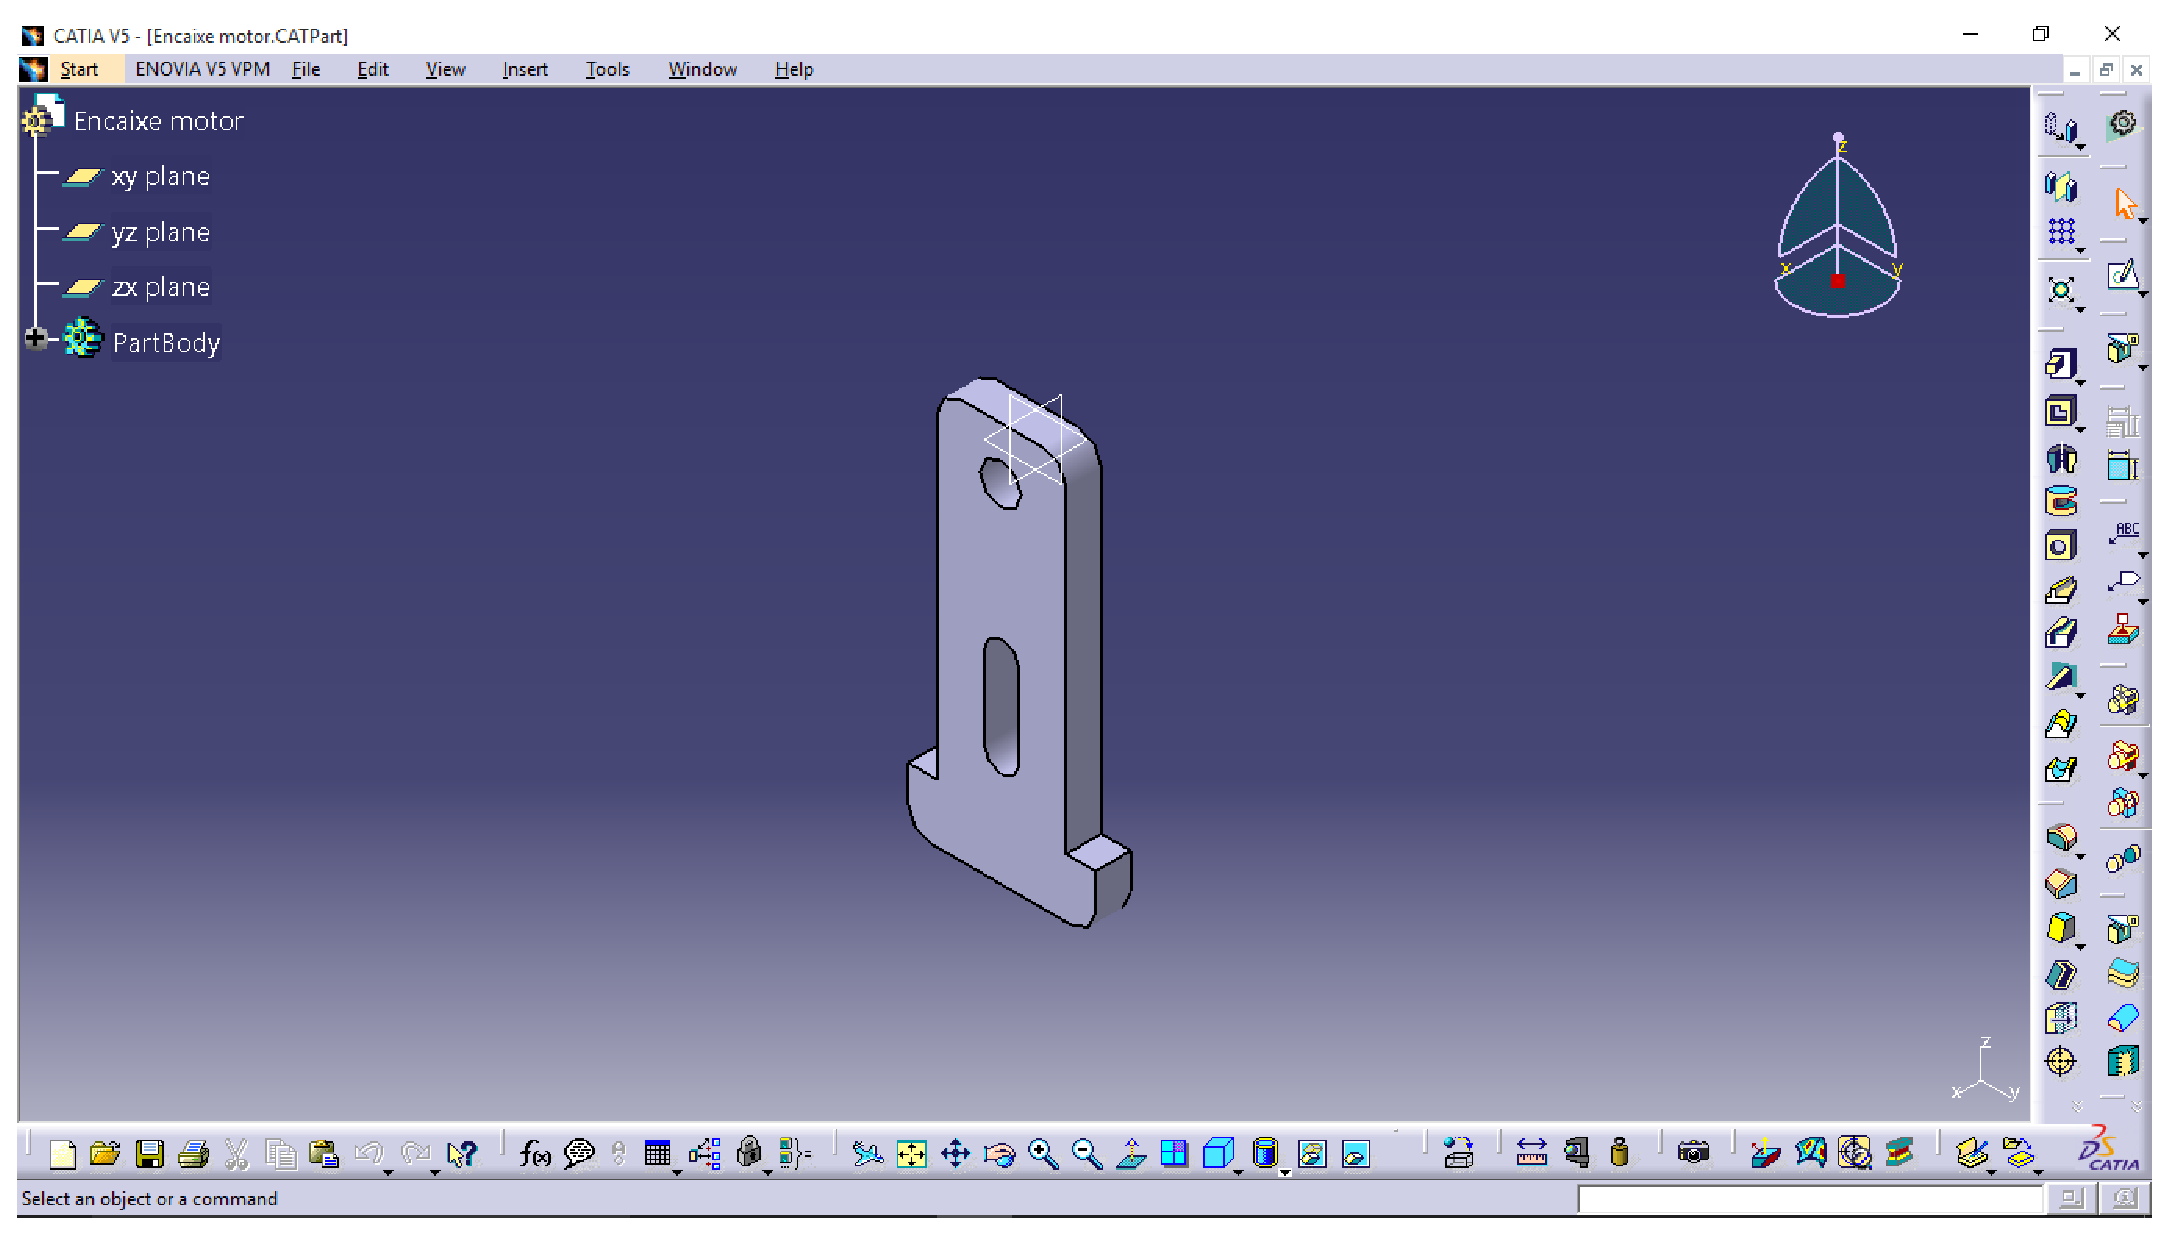
\includegraphics[width=0.7\textwidth]{figuras/sp_motor.eps}
    \caption{Suporte para os motores}
    \label{fig:sp_motor}
\end{figure}


\begin{figure}[H]
    \centering
    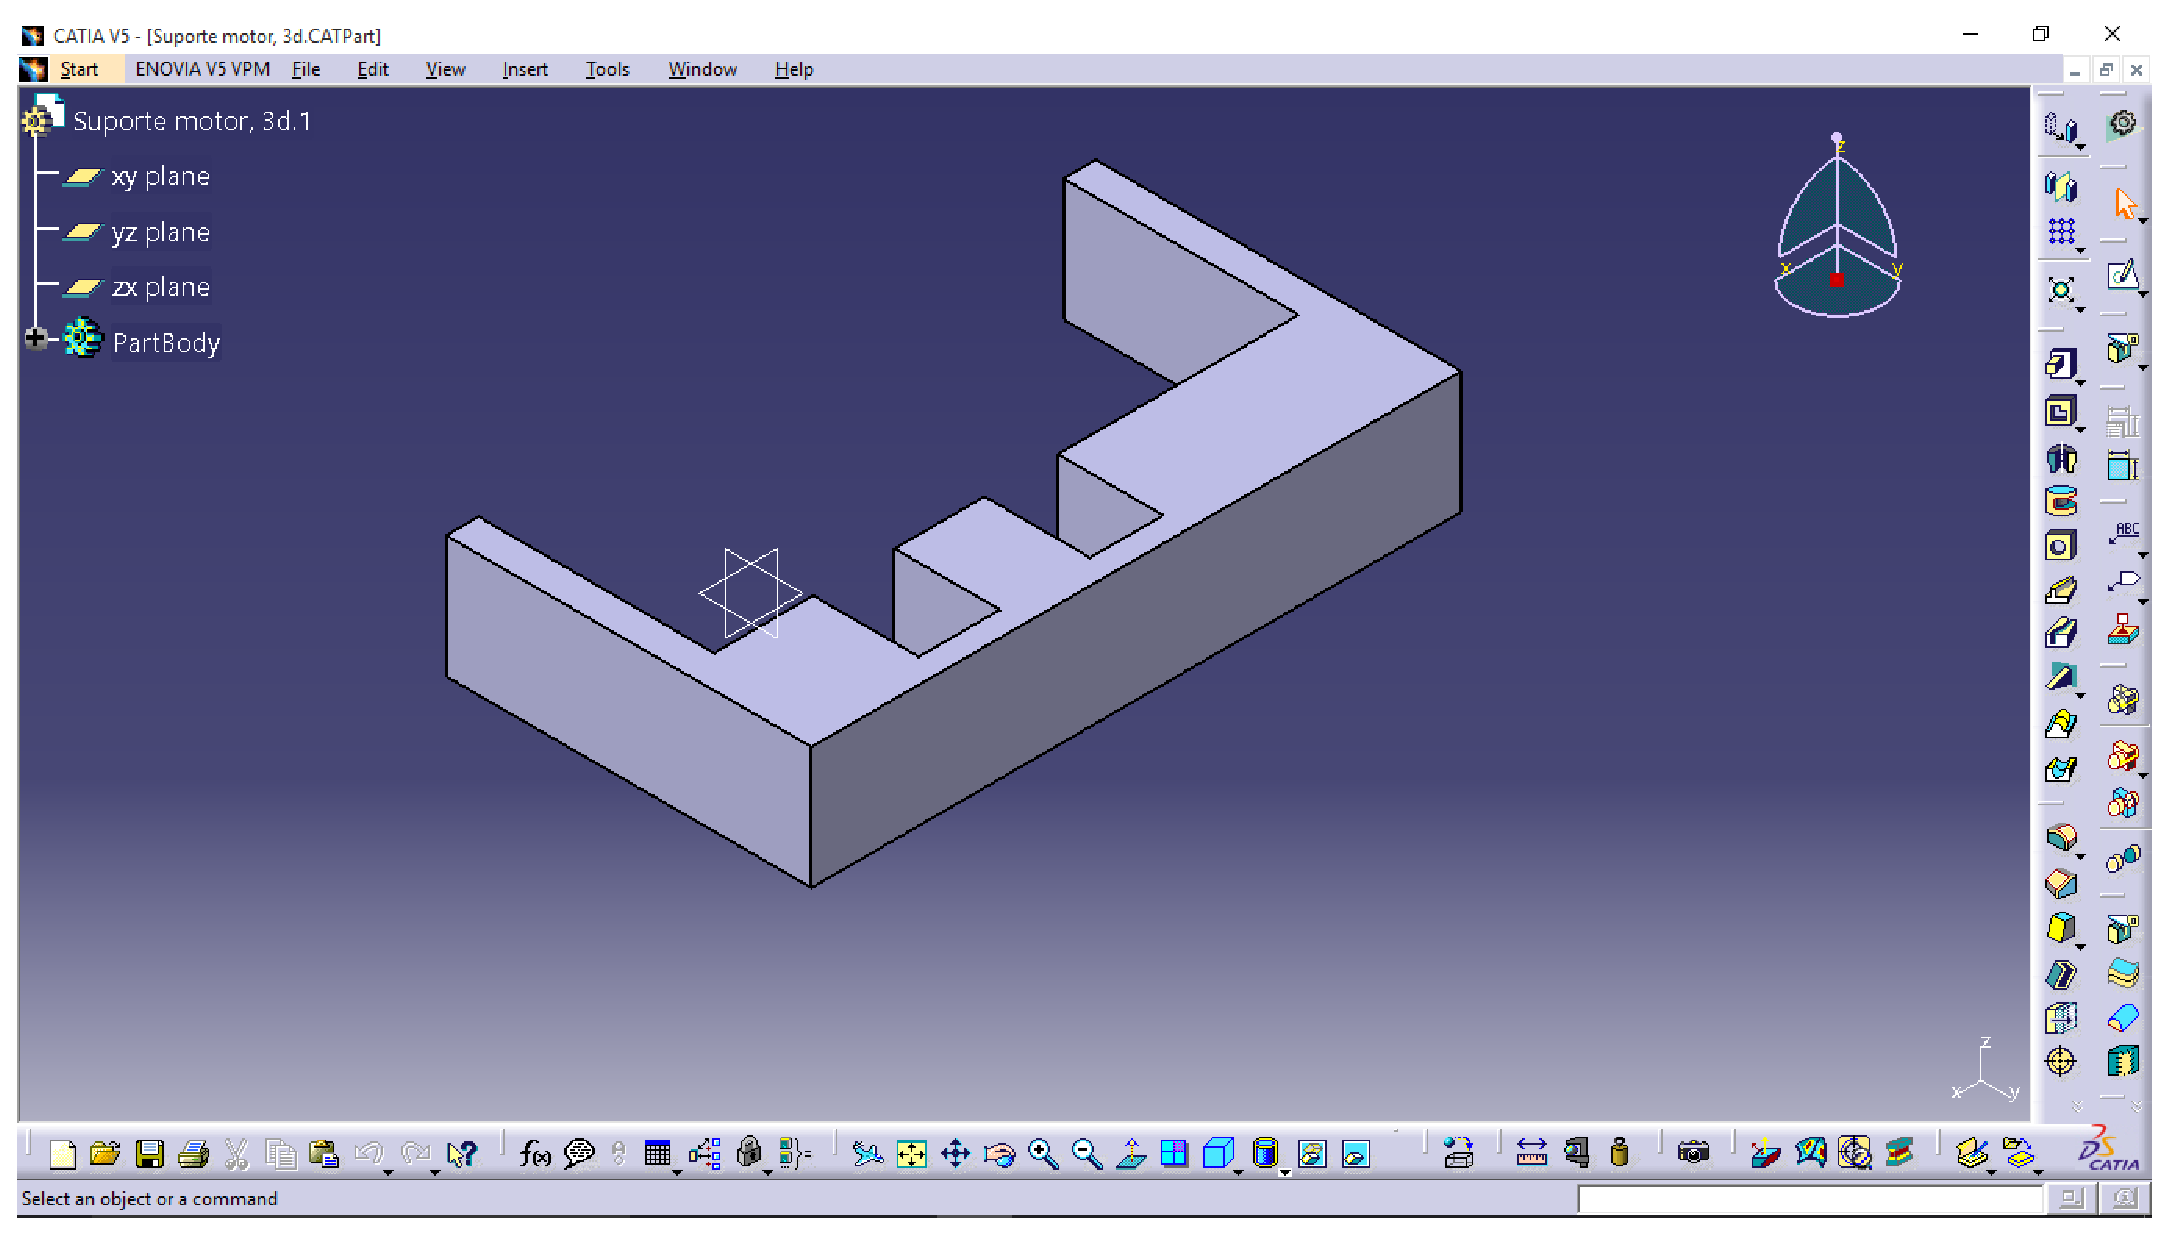
\includegraphics[width=0.7\textwidth]{figuras/en_motor.eps}
    \caption{Encaixe para os motores}
    \label{fig:en_motor}
\end{figure}

\begin{figure}[H]
    \centering
    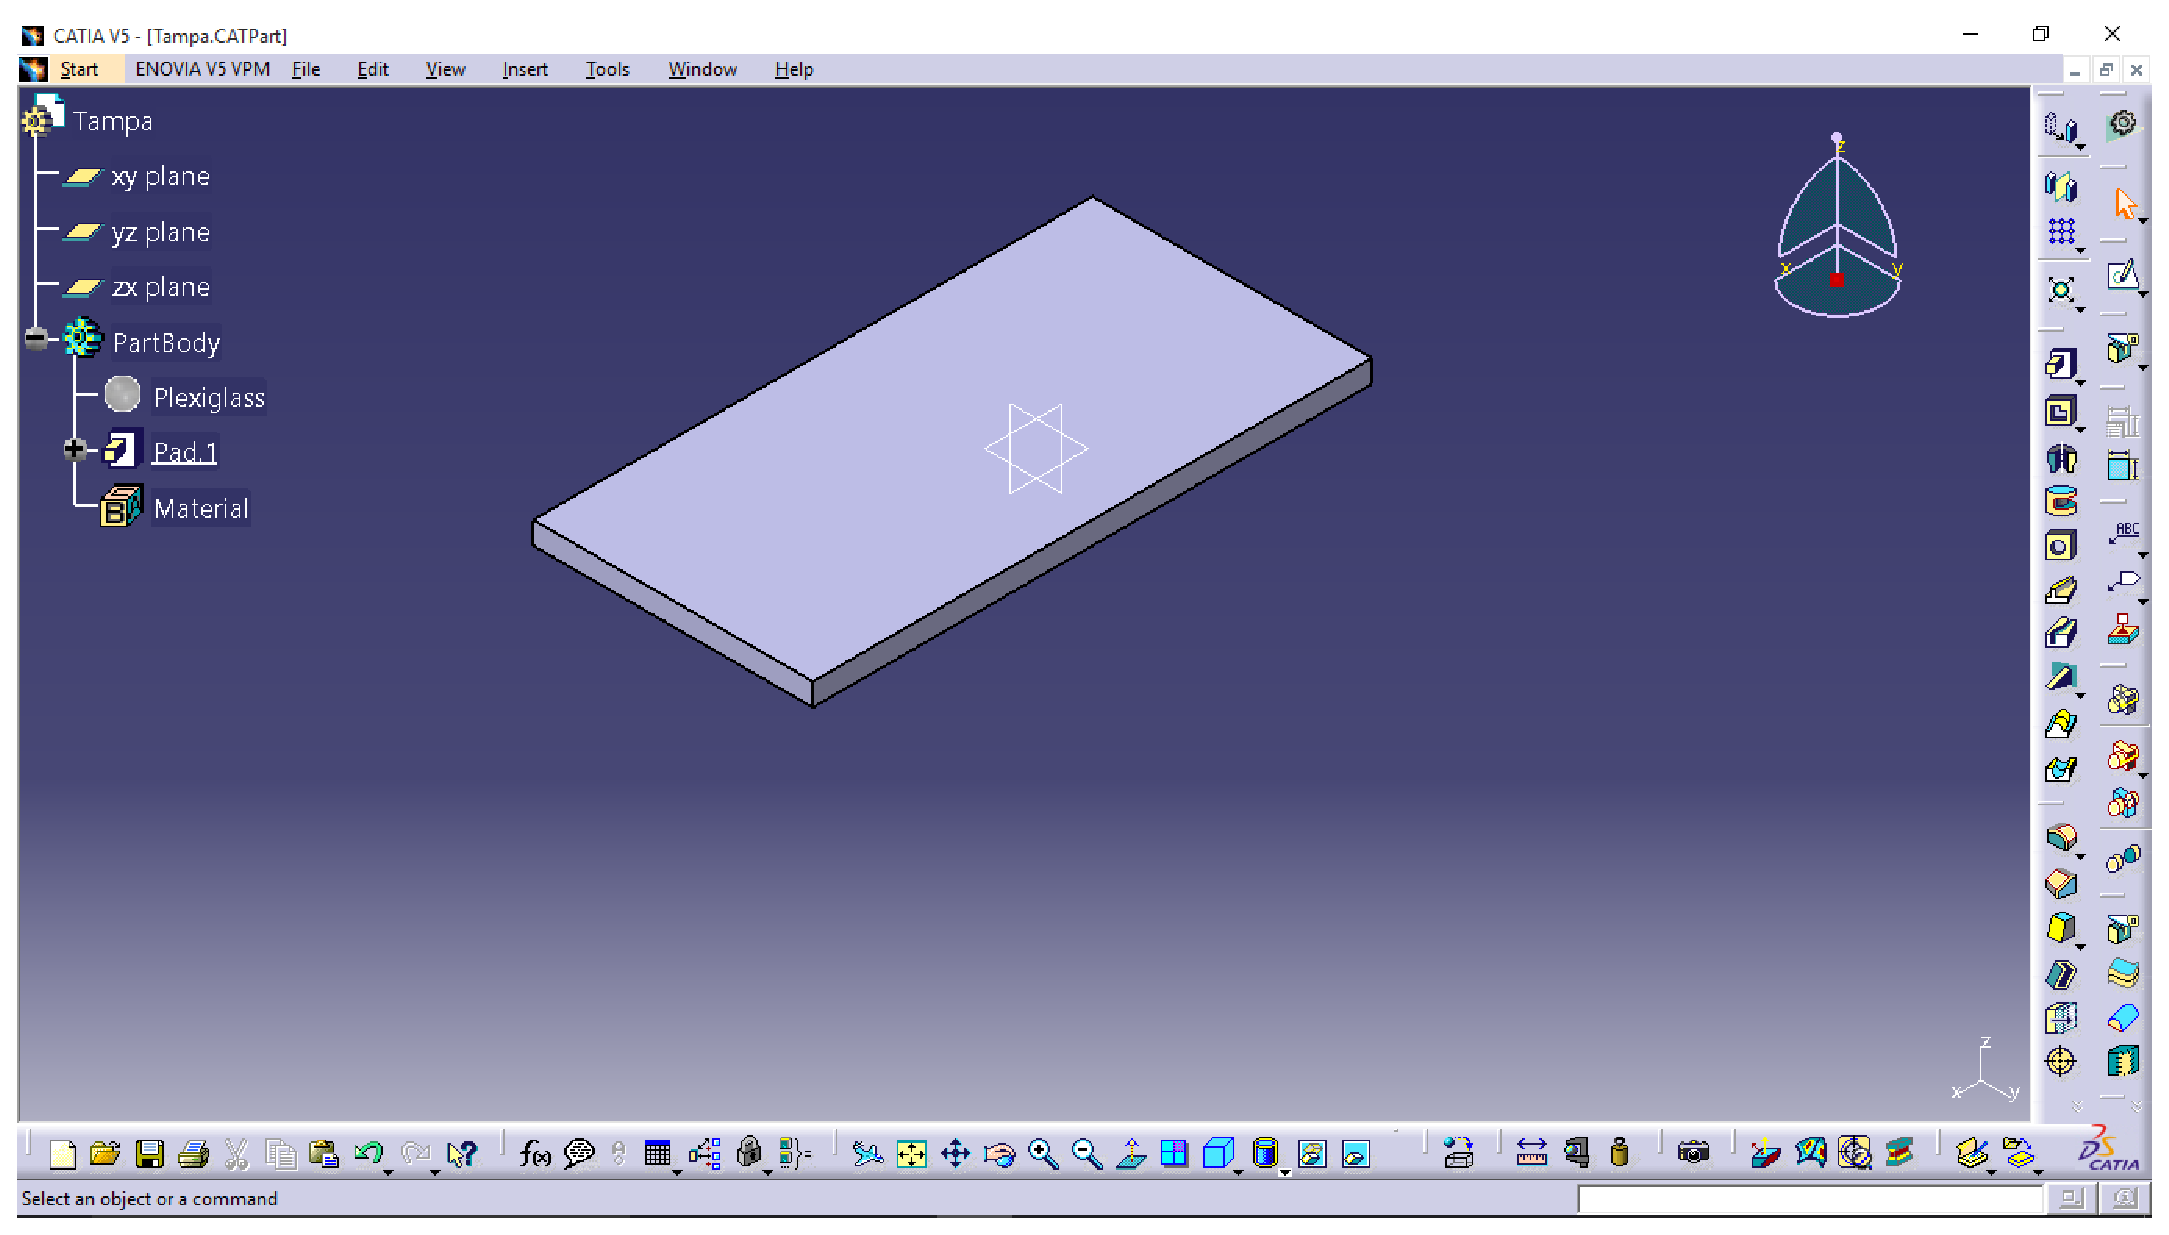
\includegraphics[width=0.7\textwidth]{figuras/tampa.eps}
    \caption{Tampa}
    \label{fig:tampa}
\end{figure}

A base de movimentação serve para alocar a maioria dos componentes eletrônicos do robô, bem como o sistema de movimentação do
mesmo. As paredes inferior e superior servem para proteger os equipamentos eletrônicos e alocar o sensor de ultrassom, a cobertura
e a tampa servem para fechar a estrutura e obter a geometria desejada, bem como para a adição de alguns efeitos como LED’s e desenhos
de modo a tornar o carrinho mais atrativo para as crianças.

\begin{figure}[H]
    \centering
    
\includegraphics[width=0.7\textwidth]{figuras/alfa_concept.eps}
    \caption{Conceito da estrutura final}
    \label{fig:alfa_concept}
\end{figure}

\subsubsection{Analise estrutural}

A análise estrutural foi realizada no software ASYNS e foi feita apenas para o caso estático. No caso dinâmico, o software
recebe os parâmetros físicos do carrinho e as condições de contorno que seria a de uma \textit{free fall}, ao final da simulação o software
retorna os valores dos parâmetros em um intervalo de tempo. Esse tipo de simulação é muito complexa e geralmente requer grande poder
de processamento. O caso estático funciona de maneira semelhante porem as condições de contorno são diferente e o resultado é valido
apenas para uma unidade de tempo, nesse tipo de simulação deve ser feita uma análise antes de maneira a obter os resultados no tempo certo.

Para realizar a análise foi importada a geometria do CATIA para i ANSYN, e foi aplicada entre as peças a condição de \textit{bonded}
(colado ou ligado), assim como foi feito na construção do chassi do carrinho.

Os parâmetros analisados foram a deformação que a estrutura sofre, e a tensão de Von Mises, de modo resumido, a teoria de tensões
de Von Mises se baseia no limite de escoamento do material. Caso o valor apresentado na escala seja menor que o limite de escoamento
do material utilizado, a estrutura estará “aprovada”.

No caso da \textbf{queda} a unidade de tempo desejada é a que a magnitude da força atuando sobre o carrinho seja a maior possível. As condições
de contorno são: um lado do carrinho sem sofrer deslocamento estrutural (deformação) e em algum outro lado aleatório (foi testado em todos
os lados) aplica-se uma força igual a força atuante na hora do impacto, esse lado representa o lado que está se chocando com o chão na hora
do impacto, os resultados da simulação são:

\begin{figure}[H]
    \centering
    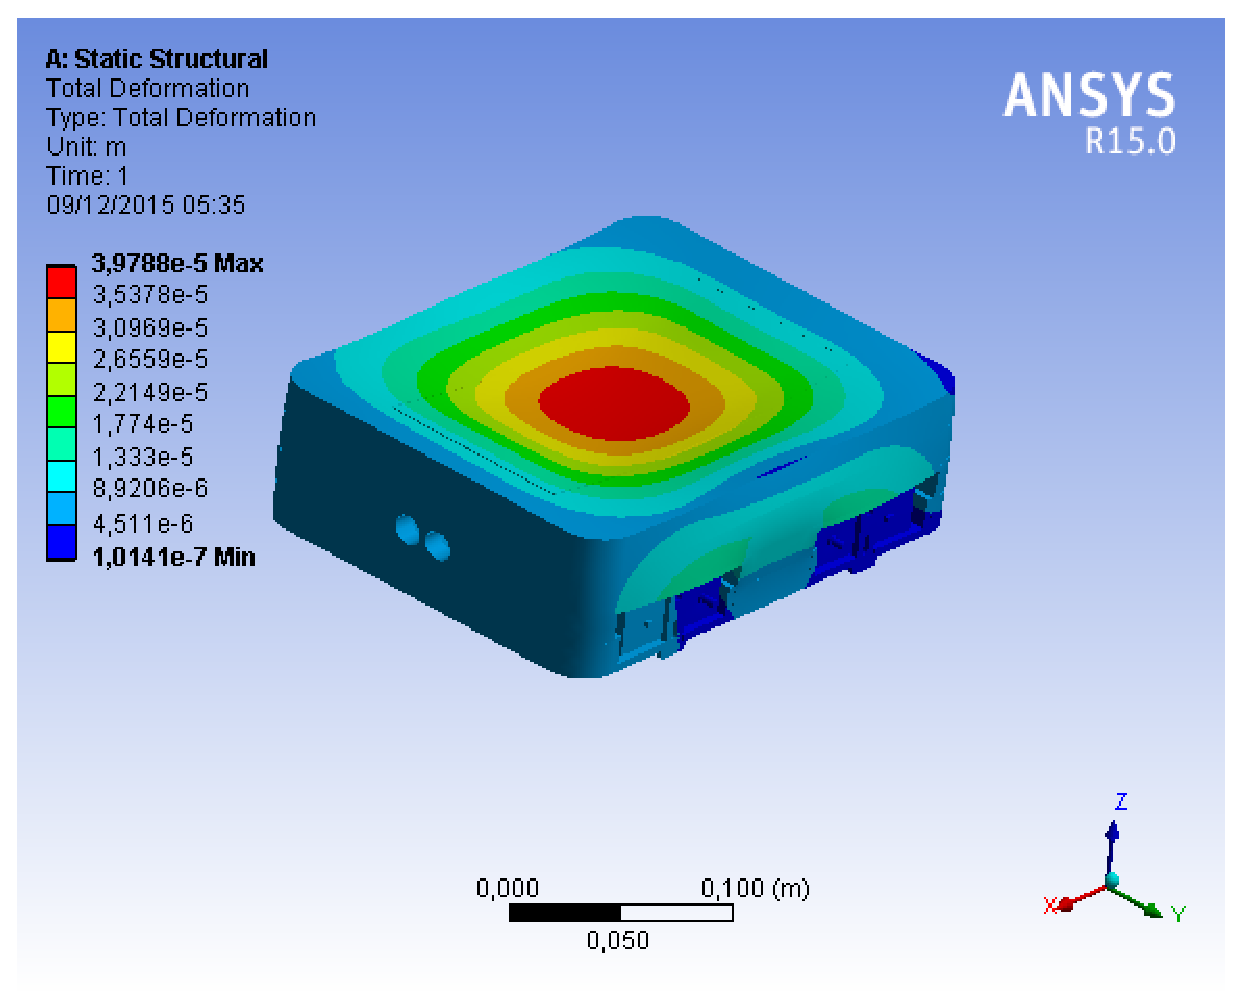
\includegraphics[width=0.7\textwidth]{figuras/queda_deformacao.eps}
    \caption{Deformação da estrutura}
    \label{fig:queda_deformacao}
\end{figure}

\begin{figure}[H]
    \centering
    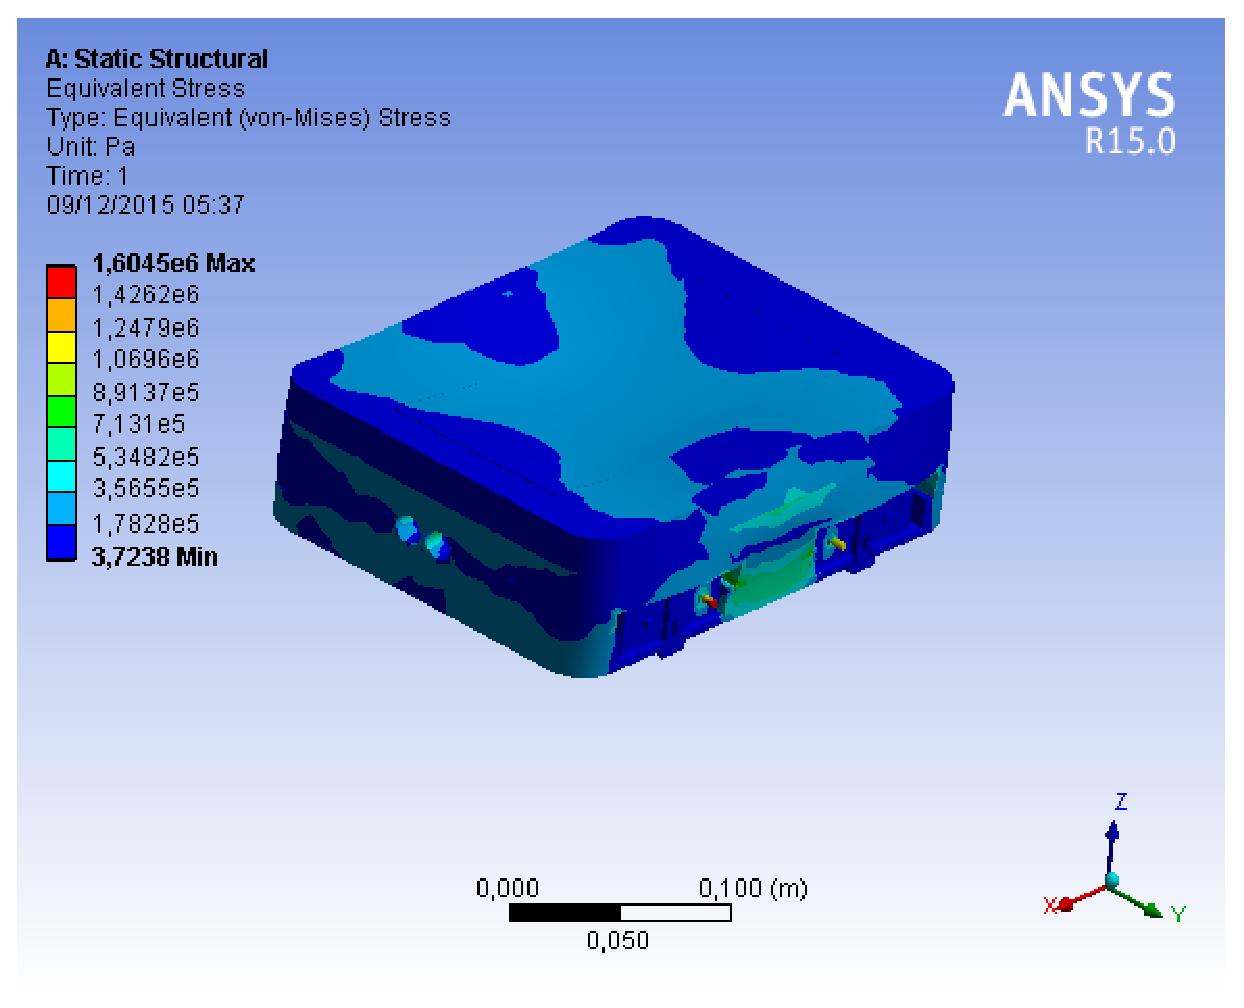
\includegraphics[width=0.7\textwidth]{figuras/queda_von.eps}
    \caption{Tensão de Von mises}
    \label{fig:queda_von}
\end{figure}

As ilustrações (Figura \ref{fig:queda_deformacao} e \ref{fig:queda_von}) apresentam as simulações cujo o lado que se chocou com o chão provoca
maior risco a estrutura. As condições de contorno são: Força de 1000 N na face superior, força de 50 N na face lateral, a face inferior e os
eixos fixos. Os valores de força não condizem com uma situação real de queda, eles foram superestimados a fim de aumentar a segurança e a
confiabilidade da estrutura. Como podemos ver não ocorre nenhum deslocamento exagerado e a superfície permanece a praticamente a mesma com
o maior deslocamento sendo da ordem de 10e-5 m, o que não apresenta nenhum risco a estrutura. Na análise do critério de Von Mises o maior
valor atingido é de 1,6 MPa o que razoavelmente próximo do valor de ruptura do MDF porém ainda é inferior, levando em consideração que as
forças da simulação estão superestimadas o que fornece um coeficiente de segurança razoável, podemos dizer que essa simulação valida a
estrutura para o caso de uma queda.

O caso estático fornece um excelente resultado para o \textbf{sobrepeso} do carrinho, pois estamos analisando a estrutura com o peso já
em cima não o comportamento da estrutura ao impacto do peso. As condições de contorno usadas na análise foram: Força de 100 N na parte
superior do carrinho, eixos e parte inferior fixa (parte que não se move). Os resultados da simulação são:

\begin{figure}[H]
    \centering
    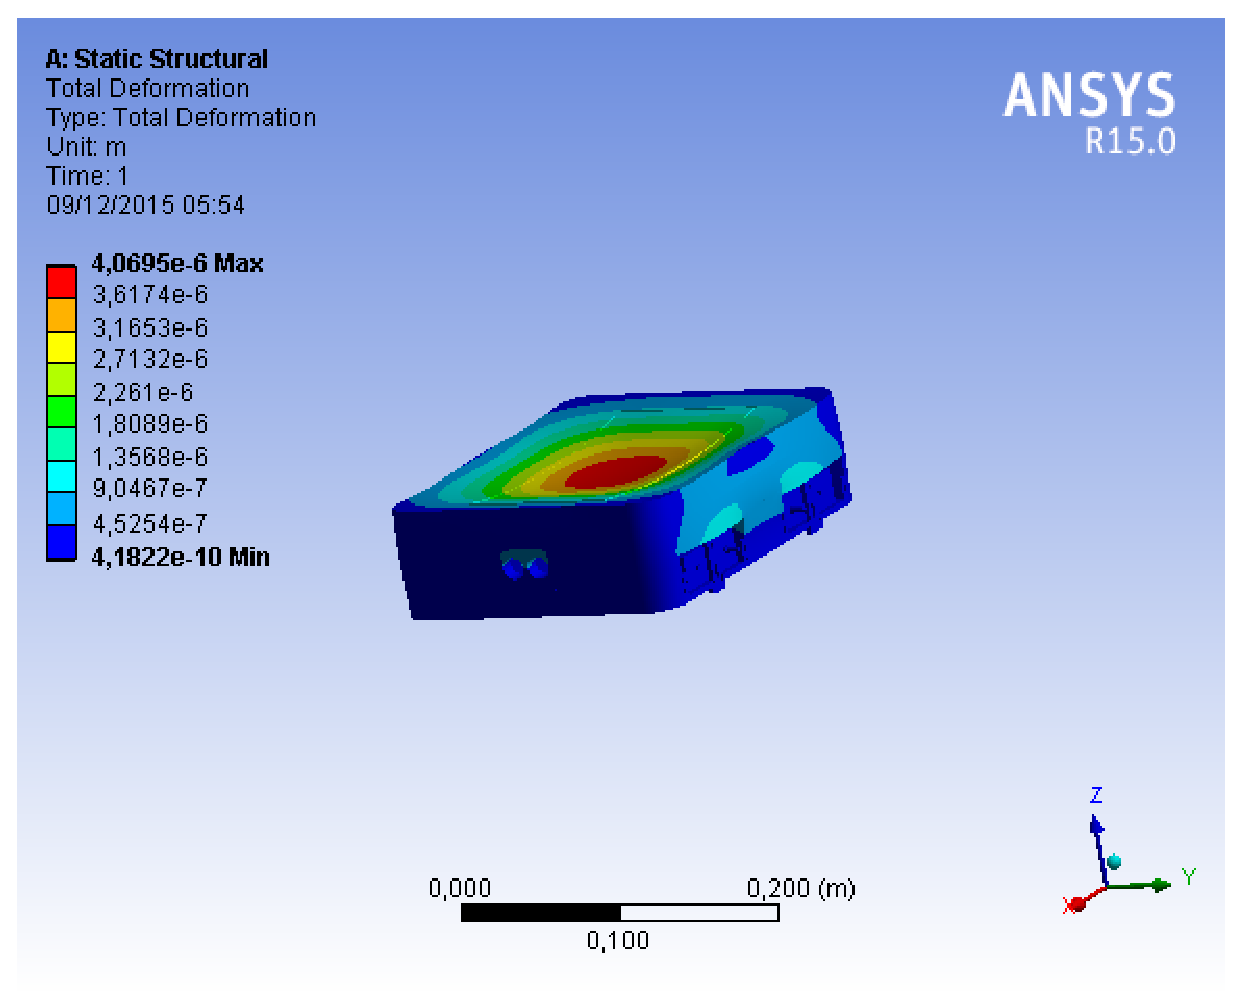
\includegraphics[width=0.7\textwidth]{figuras/sobrepeso_deformacao.eps}
    \caption{Deformação da estrutura}
    \label{fig:sobrepeso_deformacao}
\end{figure}

\begin{figure}[H]
    \centering
    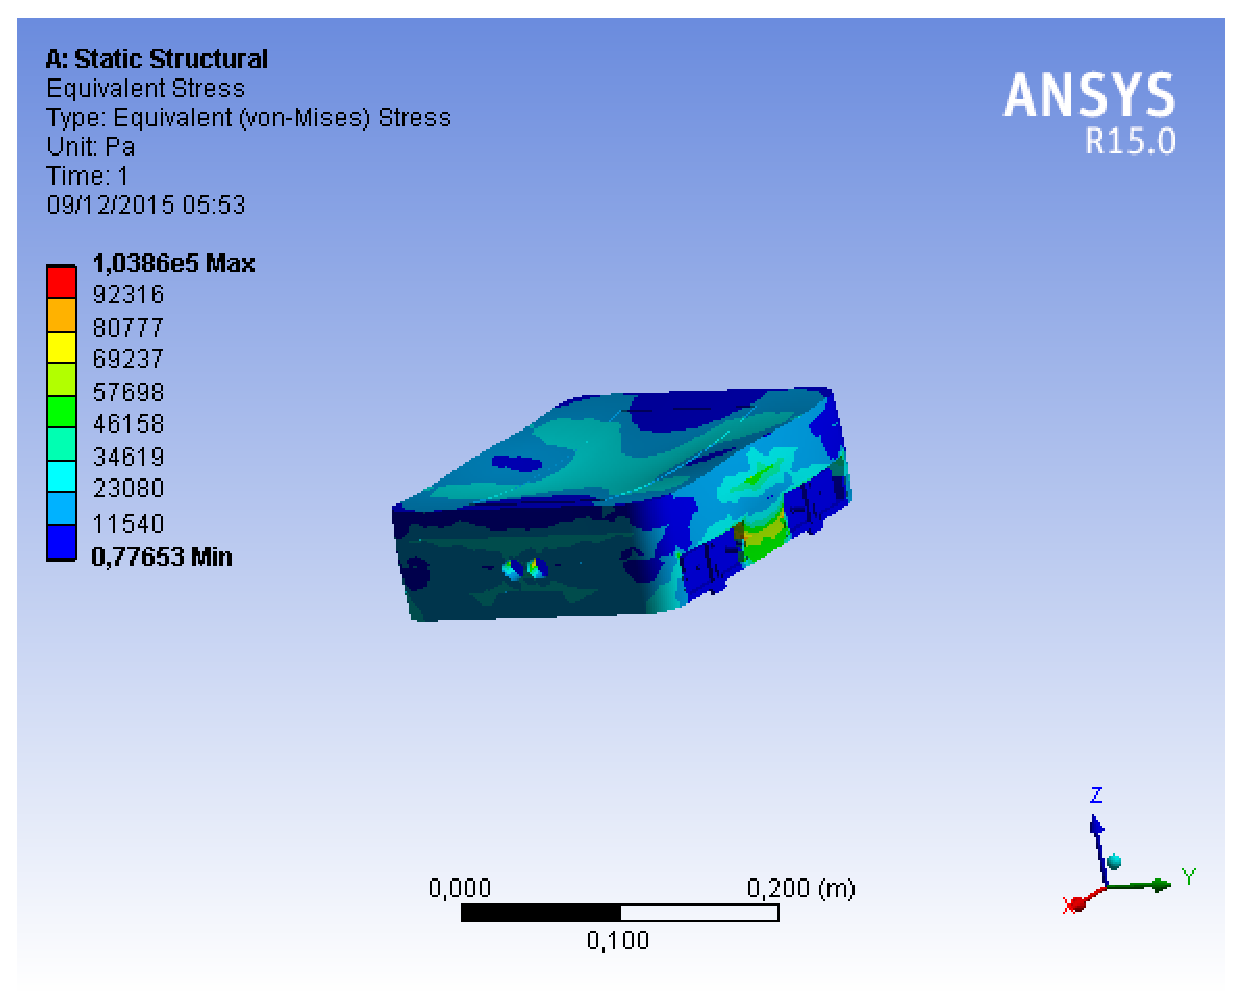
\includegraphics[width=0.7\textwidth]{figuras/sobrepeso_von.eps}
    \caption{Tensão de Von mises}
    \label{fig:sobrepeso_von}
\end{figure}

As condições de contorno para as simulações apresentadas acima são: Força de 100N na face superior da tampa e o fundo e eixos fixos. 
Como podemos ver o valor máximo da deformação é da ordem de 10e-6m o que significa que nessas condições não ocorre uma deformação expressiva
no carrinho. Os valores da tensão de Von Mises não apresentam valores que possam oferecer um real risco a integridade do material, pois
apresentam valores da ordem de 10 vezes menores que o valor da tensão de ruptura do material. Novamente essa simulação valida o uso da
estrutura no caso de um sobre peso.

\subsection{Atuadores}

Os atuadores são os componentes que convertem a energia em potência mecânica, no caso em questão utilizaremos uma bateria para alimentaçã
 do Alfa. Por meio de conversão eletromecânica a energia elétrica é convertida em potência mecânica e enviada para os elos, responsáveis
 pela movimentação do alfa.  Os atuadores utilizados em robôs de modo geral, são os atuadores eletromagnéticos, principalmente os que
 utilizam motores de corrente contínua e de passo. Os motores elétricos são interessantes no projeto de robôs, devido ao fato de que estes
 quando associado a sensores possibilitam tanto o controle de força quanto de posicionamento do robô, a facilidade na programação dos seus
 movimentos, visto que são controlados por sinais elétricos, até a utilização de controladores de movimentos \cite{romano:2002}.

Os motores elétricos são divididos basicamente em: motores de corrente alternada (ca/ac) e motores de corrente continua (cc/dc). Os motores
de corrente alternada são vantajosos devido a sua construção ser bastante simples, e a sua alimentação ocorrer diretamente da rede. No
entanto nos projetos na área da robótica os motores de corrente contínua são os mais utilizados, devido a alimentação nestes tipos de
projeto ocorrem na sua grande maioria a partir de bateria, as quais funcionam com corrente contínua, com isso a utilização de inversore
não se faz necessária \cite{braga:2006}.


Além da alimentação dos motores de corrente contínua, outras vantagens em sua utilização, são devidos \cite{braga:2006}:.
\begin{itemize}
	\item a velocidade do motor ser ajustada a partir de um potenciômetro, realizando a variação da tensão aplicada sobre o motor;
	\item o sentido de rotação do motor pode ser alterado a partir da mudança de polaridade da tensão aplicada ao motor;
	\item ao controle da aceleração e desaceleração do motor promovendo uma resposta no tempo ou para suavizar o funcionamento deste;
	\item a possibilidade de controle do torque a partir da variação da corrente aplicada no motor;
	\item a apresentarem uma resposta rápida, ou seja, quando submetidos a voltagens elevadas acelera rapidamente.
\end{itemize}

Os motores utilizados no Alfa são motores dc, com caixa de redução 1:48, e eixo duplo, a escolha desse motor ocorreu devido aos
fatores apresentada acima. A tabela (Figura fig:tensao) apresentado as especificações do motor que será utilizado.

\begin{figure}[H]
    \centering
    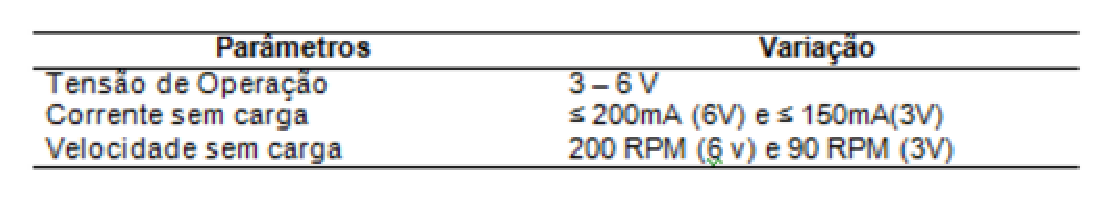
\includegraphics[width=0.8\textwidth]{figuras/tensao.eps}
    \caption{Especificações dos motores utilizados no Alfa.}
    \label{fig:tensao}
\end{figure}

\begin{figure}[H]
    \centering
    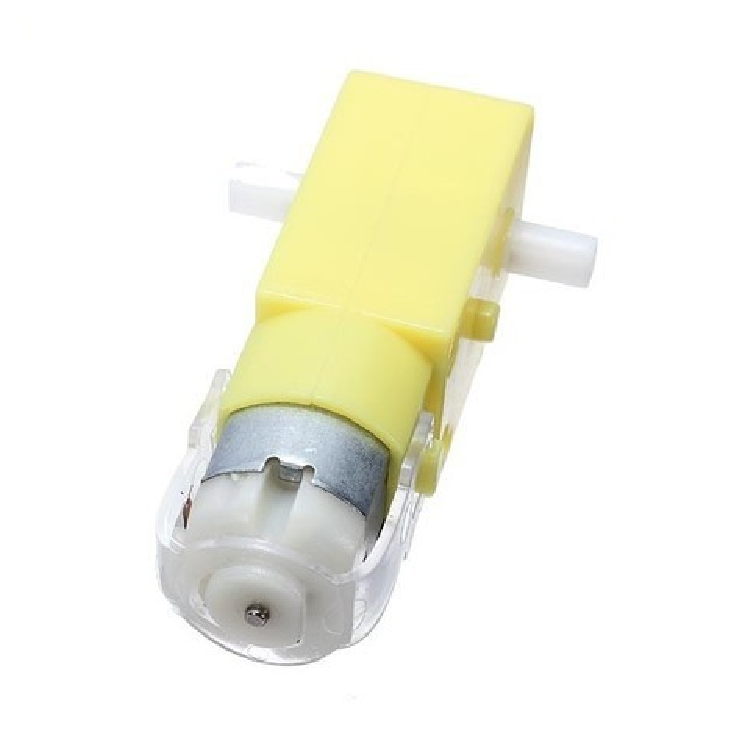
\includegraphics[width=0.6\textwidth]{figuras/motor.eps}
    \caption{Motor utilizado no robo Alfa. Fonte: Amazon S3 Web Services}
    \label{fig:motor}
\end{figure}

\subsection{Alimentação}

A alimentação dos componentes será feita por intermédio da placa Raspberry pi, o levantamento das necessidades energéticas delimitou
que a placa necessita de uma tensão constante em 5 volts, recebendo 2 ampères de corrente.  Assim surgiram duas opções de
alimentação: Pilhas ou Baterias.

As pilhas podem ser divididas em recarregáveis e não recarregáveis. As pilhas recarregáveis apesar de mais caras, possuem a vantagem de
serem usadas em centenas de ciclos de carga e recarga. As de uso único tornam o projeto mais barato, entretanto o custo de troca de
pilhas reaparece várias vezes para o consumidor. Independentemente do tipo de pilha utilizada, as pilhas comerciais apresentam valores
de tensão e corrente muito abaixo do necessário, sendo necessário colocar várias em série para elevar a tensão e várias em paralelo,
para elevar a corrente de alimentação. Isso acaba tornando o uso de pilhas nada prático.

Além de que a tensão de pilhas cai de acordo com a capacidade é utilizada, fazendo com que a placa desligasse antes da pilha estar
totalmente carregada pelo fato da tensão não estar adequada, a figura abaixo ilustra (para uma pilha AA “heavy duty”).

\begin{figure}[H]
    \centering
    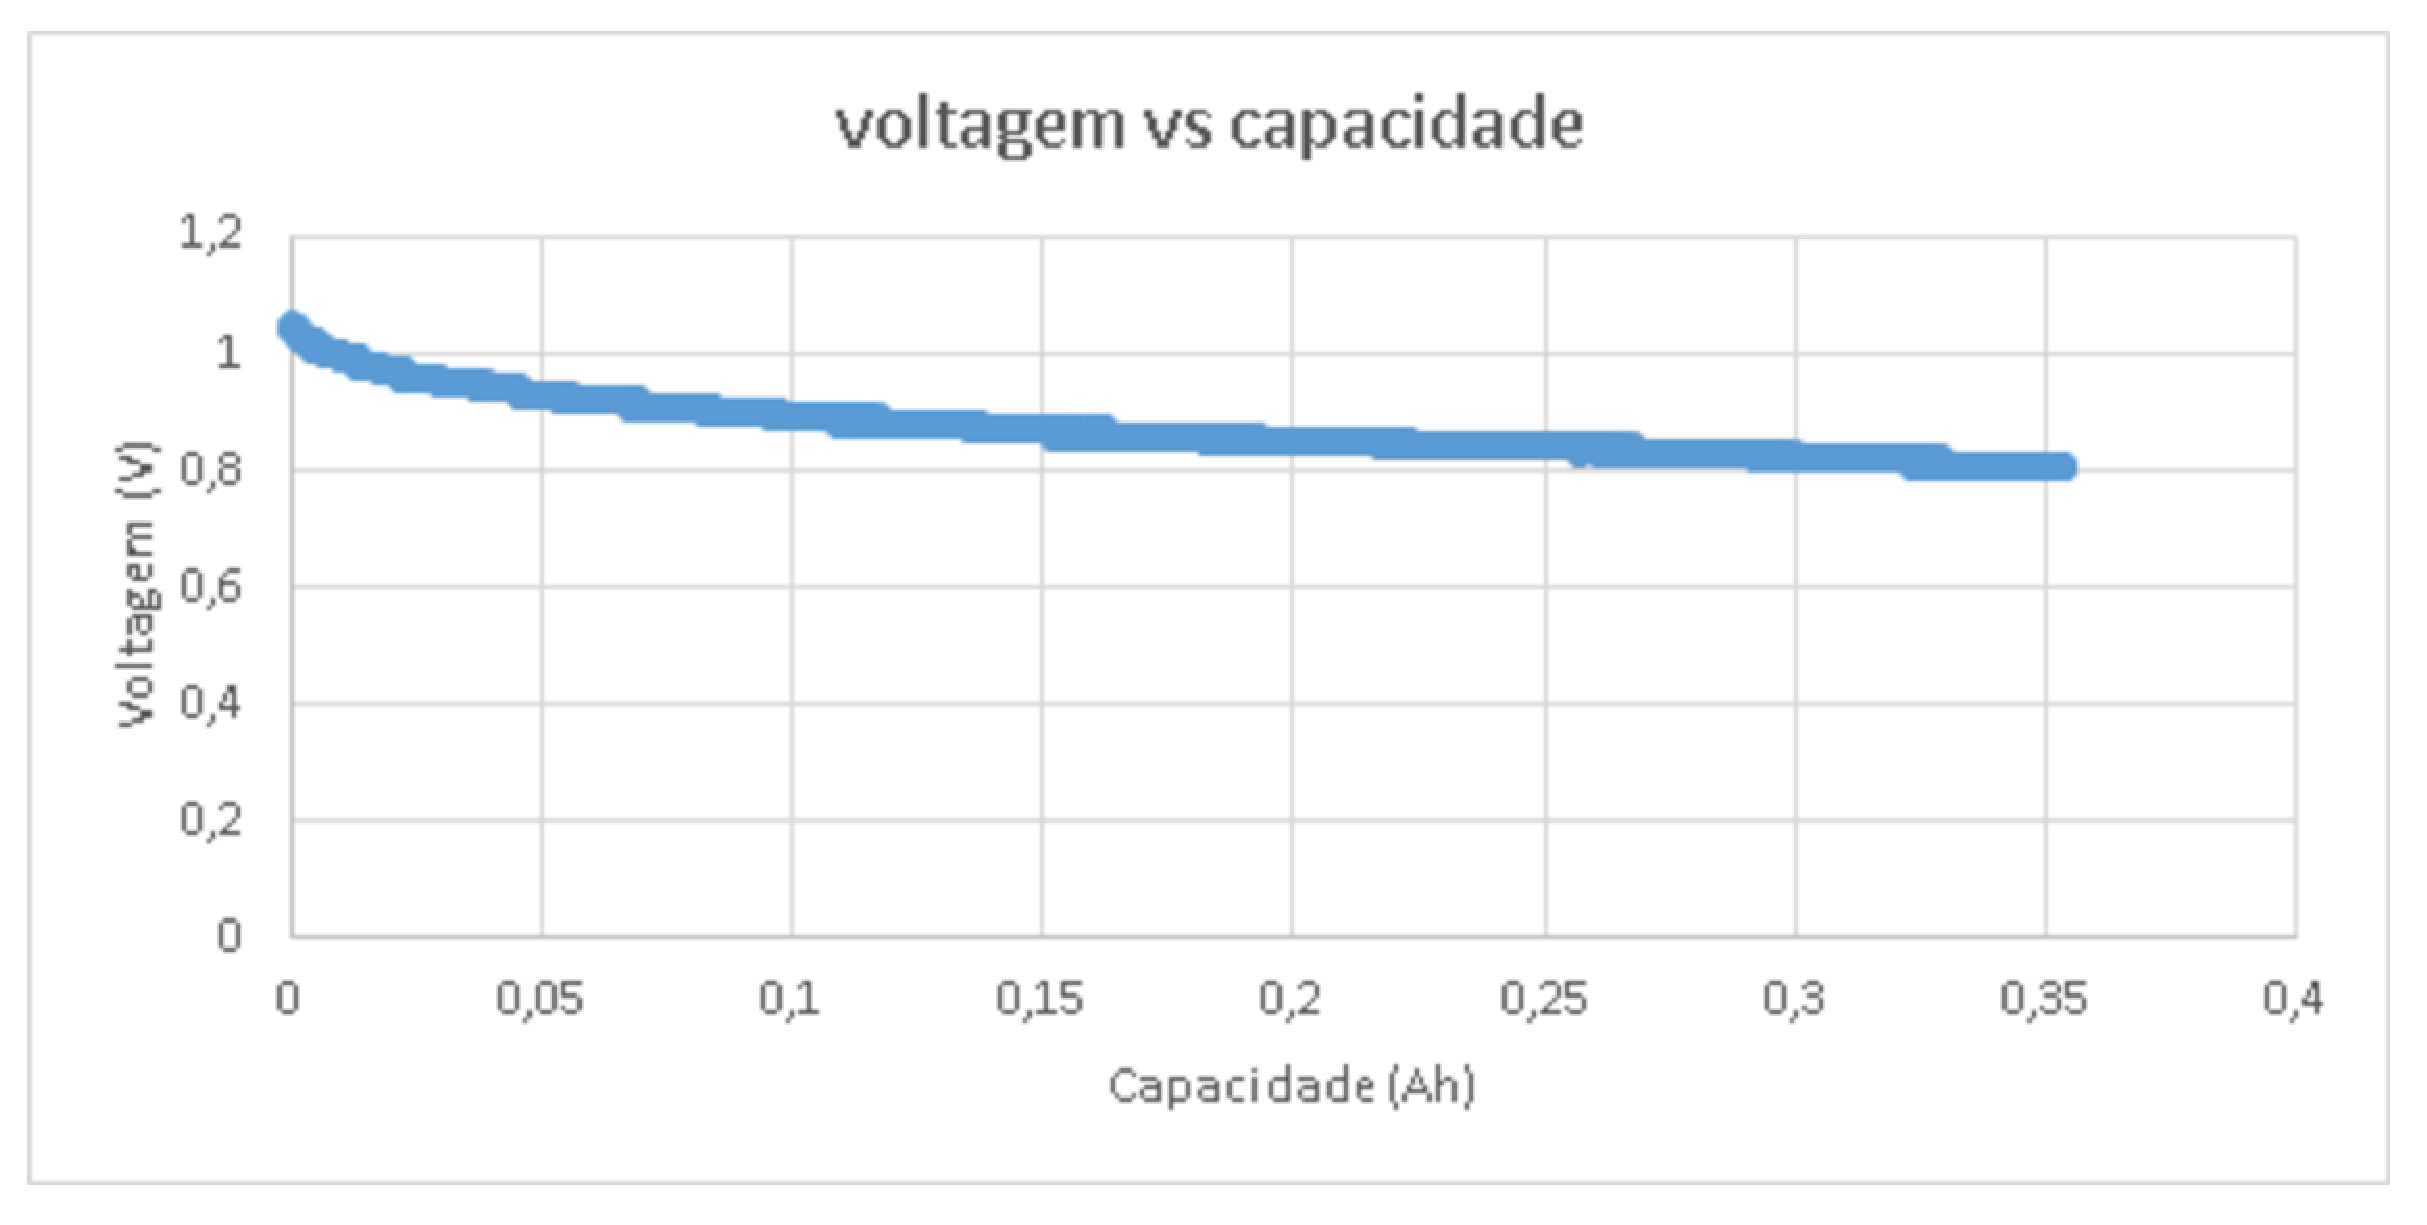
\includegraphics[width=0.8\textwidth]{figuras/volt_vs_cap.eps}
    \caption{curva de tensão sob a capacidade de uma pilha AA}
    \label{fig:volts}
\end{figure}

As baterias encontradas no mercado podem ser de vários tipos, as mais comuns são as de íon-Lítio, a maior vantagem delas é o seu fator
energético em função do peso ser alto, elas costumam ser bem mais leves que outras baterias recarregáveis de mesmo tamanho (geralmente
150 watt-hora para cada quilo de bateria), além de serem bem mais baratas e seguras que outras baterias, como as de chumbo-ácido.

A bateria escolhida é a KMASHI MP816, por apresentar uma capacidade nominal de 10 Ah, atendendo ao projeto. Sua recarga é rápida e sua 
descarga pode ser controlada de acordo com a necessidade do projeto.  Para verificar se a carga real era próxima da nominal, um teste
de carga foi realizado. O peso da bateria é de 280 gramas.

Ao se manter uma tensão constante de 5V e 2A (totalizando 10W de potência nominal para recarga) a bateria necessitou de em média 3 horas
para atingir uma carga satisfatória (90\% da carga), em uma alimentação forçada de 4 horas, o nível de carga subiu pouco (em torno de 5\%)
comparado às 3 horas iniciais. Logo o sistema possui um tempo de recarga para valores satisfatórios de 3 horas quando se utiliza uma fonte
D.C. de 10 watts de potência. Para a descarga, o sistema apresenta um valor um pouco inferior. 2 horas e 50 minutos de autonomia em média,
considerando que a carga será constante de 10,5 watts.

Para alimentar a placa Raspberry Pi a porta 1 da bateria foi utilizada, por fornecer 5 volts de tensão e uma corrente de até 1 A, a
conexão da bateria com a placa foi feita utilizando um conector USB - micro USB devido as características de entrada e saída do Raspberry
pi e da bateria. Logo, a ponte H ficou com a porta 2 da bateria, que fornece uma corrente de até 2,1 A, a maior capacidade da porta 2
permite que os motores desenvolvam uma maior potência quando comparado à conexão na porta 1.

\begin{figure}[H]
    \centering
    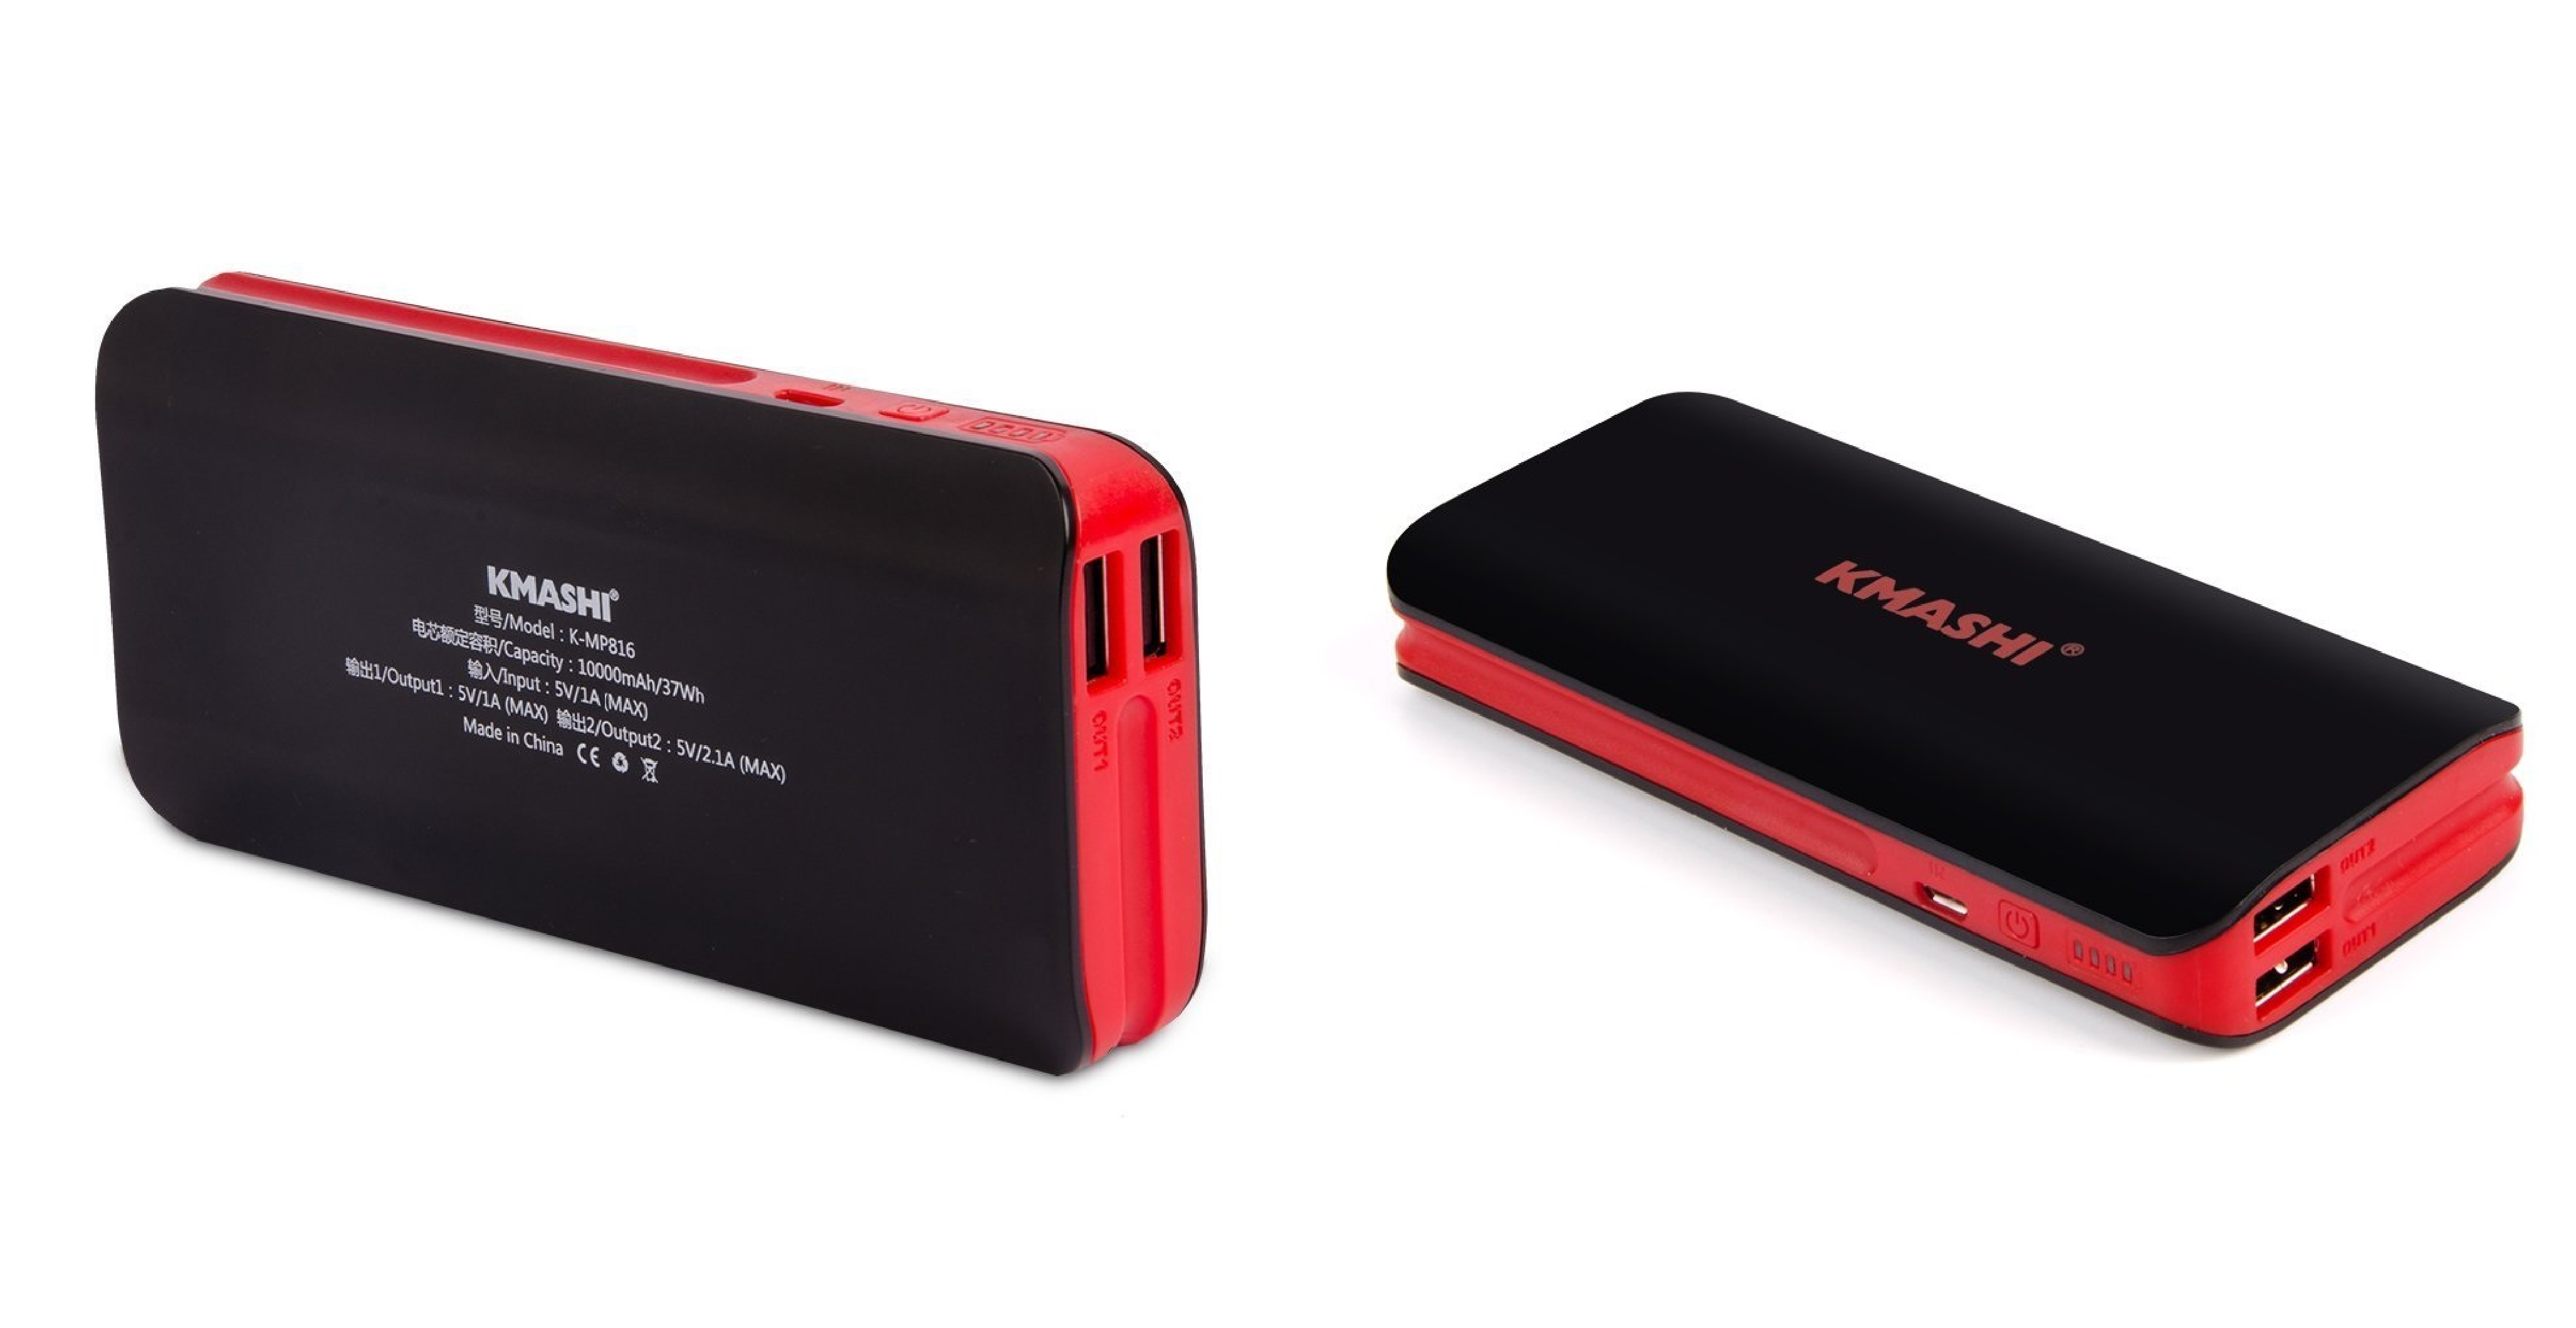
\includegraphics[width=0.9\textwidth]{figuras/baterias.eps}
    \caption{Modelo de bateria}
    \label{fig:bateria}
\end{figure}

\subsection{Sitema de Locomoção}

O ambiente de trabalho de um robô móvel é a característica que mais impõe restrições sobre o seu sistema de locomoção, portanto estes
precisam se adaptar ao seu meio físico quando são projetados. Os mecanismos de locomoção dos robôs móveis são adaptados de acordo com
o seu ambiente de trabalho. Os robôs móveis podem apresentar a capacidade de andar, saltar, correr, arrastar, deslizar, nadar, voar
e rolar \cite{secchi:2008}.

O tipo de locomoção do robô móvel é um fator determinante no seu comportamento, definindo a sua interação com o ambiente no qual
este se locomove. A estabilidade estática e dinâmica dos robôs móveis está ligada ao número e configuração dos pontos de contanto,
as características de atrito, ao centro de gravidade e a inclinação do terreno \cite{silva:2010}.

Segundo \citeonline{secchi:2008}, o ambiente de trabalho dos robôs móveis é agrupado segundo a área de trabalho e segundo os objetos
presentes no ambiente. Segundo a área de trabalho, o ambiente pode ser interior ou exterior. O ambiente é interior quando a sua
área de operação é definida por paredes e tetos e exterior quando está área de operação não é delimitada. Segundo os objetos
presentes no ambiente do robô, este pode ser classificado em estruturado ou não estruturado.

O ambiente é estruturado quando os objetos presentes no meio são estáticos, ou seja, não apresentam mudança na sua forma, nem na
sua posição apresentando características particulares permitindo associar a estes uma forma geométrica conhecida, sendo capaz de
distingui-los de outros objetos. O ambiente e não estruturado quando o entorno é dinâmico, ou seja, muda com o decorrer do
tempo, sendo tais mudanças imprevisíveis e a determinação das características físicas são inviáveis \cite{secchi:2008}.

\begin{figure}[H]
    \centering
    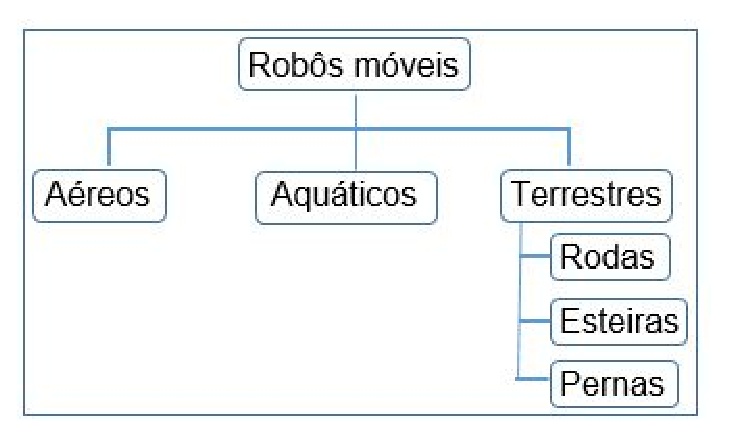
\includegraphics[width=0.6\textwidth]{figuras/locomocao.eps}
    \caption{Tipos de sistemas de locomoção de um robo móvel.}
    \label{fig:locomocao}
\end{figure}

Segundo \citeonline{pieri:2002}, o ambiente de trabalho de um robô móvel pode ser aéreo, aquático ou terrestre. A classe de robôs
terrestres pode ser dividida em três: com rodas, com esteiras ou com pernas, como pode ser observado na Figura \ref{fig:locomocao}.

Os robôs aéreos de modo geral são utilizados para inspeção em grandes áreas, sendo equipados com câmeras de vídeo.  Os robôs aquáticos
usualmente são plataformas equipadas com balões de ar e propulsores permitindo ao robô permanecer submerso a alguns metros do fundo do
mar \cite{pieri:2002}.

Os robôs terrestres são os mais populares. A locomoção por esteira é a mais utilizada quando o robô móvel é submetido a ambientes
irregulares, tem como principal desvantagem há dissipação de energia oriunda do movimento de giro da própria esteira e das rodas em seu
interior. A locomoção por pernas é a mais utilizada quando o robô móvel é submetido a ambientes acidentados, com subidas íngremes, a
principal desvantagem deste tipo de locomoção é a complexidade de implementação deste sistema mecânico bem como no seu controle \cite{pieri:2002}.

A locomoção por rodas é o tipo mais utilizado em robôs móveis, devido a sua simplicidade e sua estabilidade uma vez que os robôs com
rodas são concebidos para que estas sempre permaneçam em contato com o solo, a sua principal desvantagem é a dificuldade de locomoção
em ambientes não estruturados \cite{pieri:2002} \cite{siegwart:2002}. 

O tipo de roda e a disposição destas na estrutura mecânica influenciam na sua mobilidade e no seu comportamento cinemático, uma vez
que as rodas podem impor restrições ou permitir o movimento da estrutura em determinadas direções. As rodas convencionais e a sueca
(swedish wheel) são basicamente as duas classes de rodas (SECCHI, 2008). As rodas convencionais por sua vez são divididas em: roda fixa,
roda orientável centralizada e roda castor como pode ser observado na Figura \ref{fig:roda}.

\begin{figure}[H]
    \centering
    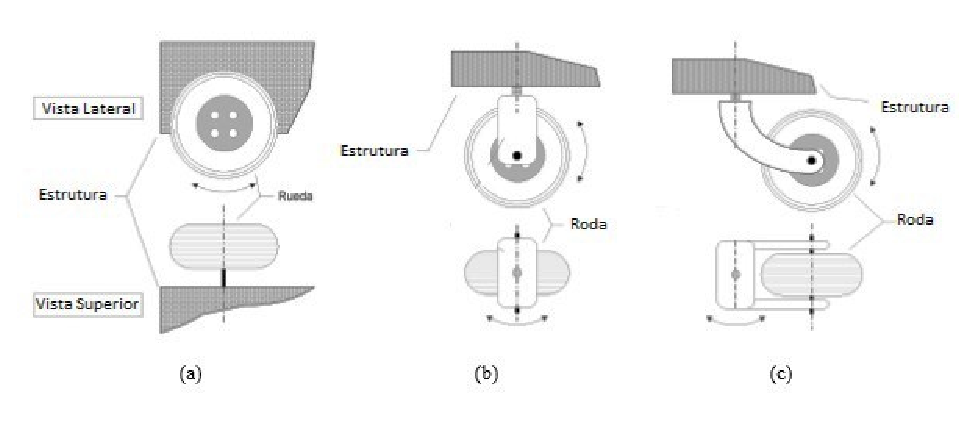
\includegraphics[width=0.9\textwidth]{figuras/roda.eps}
    \caption{Tipos de rodas. (a) Roda fixa. (b) Roda orientável centralizada. (c) Roda castor. Fonte: SECCHI, 2008.}
    \label{fig:roda}
\end{figure}

As rodas fixas têm o seu eixo fixado na estrutura do robô como pode ser observado na Figura \ref{fig:roda}.a. As rodas orientáveis centralizada
apresentam rotação ao redor do seu eixo vertical que passa através do centro da roda, como pode ser observado na Figura \ref{fig:roda}.b. As
rodas castor são orientada com relação à estrutura de tal modo que o seu eixo vertical não passa através do centro da roda, como
pode ser observado na Figura \ref{fig:roda}.c \cite{secchi:2008}. 

O arranjo e a geometria das rodas na estrutura influenciam na escolha do tipo de roda. As características fundamentais a serem
consideradas nessa escolha são: a estabilidade, manobridade e controlabilidade. A Figura T fornece uma visão geral das configurações
de rodas ordenadas por número, apresentando desde uma seleção particular dos tipos de rodas bem como sua distribuição espacial na estrutura.

\begin{figure}[H]
    \centering
    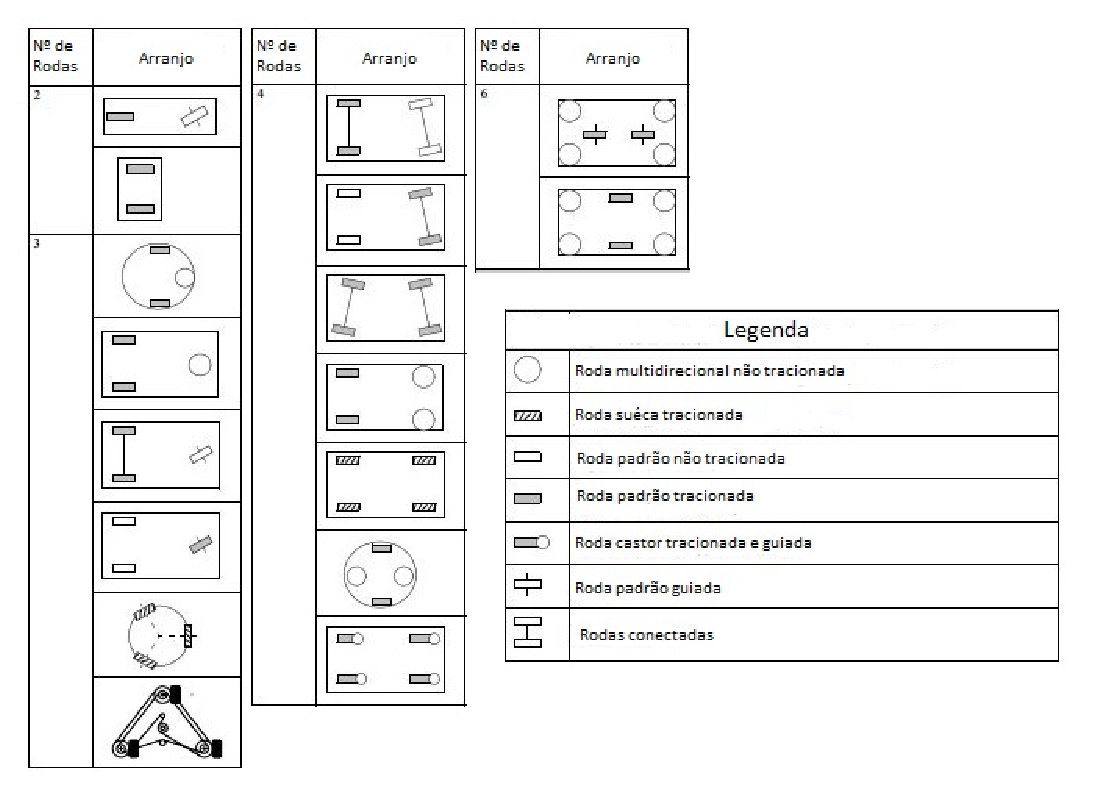
\includegraphics[width=0.9\textwidth]{figuras/arranjos_roda.eps}
    \caption{Tipos de arranjos de rodas possíveis para robôs móveis. Fonte: SIEGWART \& NOURBAKHSH, 2004}
    \label{fig:arranjo_roda}
\end{figure}

A estabilidade estática dos robôs móveis convencionalmente ocorre com a utilização de no mínimo três rodas, de forma que sua disposição
na estrutura são rodas em paralelo de modo que o centro de massa esteja contido no triângulo formado pelos pontos de contato solo com a
roda. A adição de mais rodas na estrutura aumenta a estabilidade, no entanto a inclusão de mais rodas torna a estrutura super estática.
A manobrabilidade do robô é diretamente proporcional a quantidade de graus de liberdade das rodas. A controlabilidade por outro lado é
inversamente proporcional a manobrabilidade \cite{braga:2014}.

Não é possível idealizar um arranjo, no qual é se maximize simultaneamente a estabilidade, manobrabilidade e a controlabilidade.
Fica a cargo do projetista avaliar as configurações necessárias afim de se aproximar das condições ideais. A disposição de rodas deste
projeto foi baseada na análise crítica das propriedades fundamentais para o funcionamento do robô no seu ambiente de trabalho. Duas opções
foram consideradas: a utilização de duas rodas tracionadas e uma roda boba; e a utilização de quatro rodas tracionadas. A segunda opção foi
a escolhida devido ambiente doméstico ser delimitado e estruturado, outro ponto analisado para o projeto foi a manobrabilidade a qual não
é um fator determinante para este, uma vez que fica a cargo do usuário está funcionalidade.

\begin{figure}[H]
    \centering
    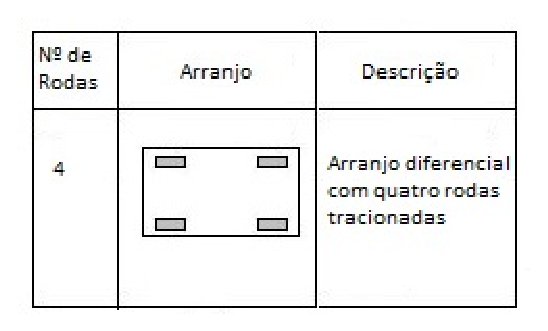
\includegraphics[width=0.6\textwidth]{figuras/arranjo.eps}
    \caption{Arranjo das rodas selecionadas}
    \label{fig:arranjo}
\end{figure}


\section{Visão e Controle e Processamento}

Esta seção mostra os itens relacionados ao controle e processamento dos dados de comunicação do sistema. O sistema, em uma visão ampla
(figura \ref{fig:overview_down}), é dividido em dois subsistemas:

\begin{itemize}
\item Inserido no \textbf{raspberry}, responsável por realizar a interpretação e execução do conjunto de instrução do programa;
\item Inserido no aparelho \textbf{Android}, responsável pela construção dos programas contendo os conjuntos de instruções;
\end{itemize}

\begin{figure}[H]
    \centering
    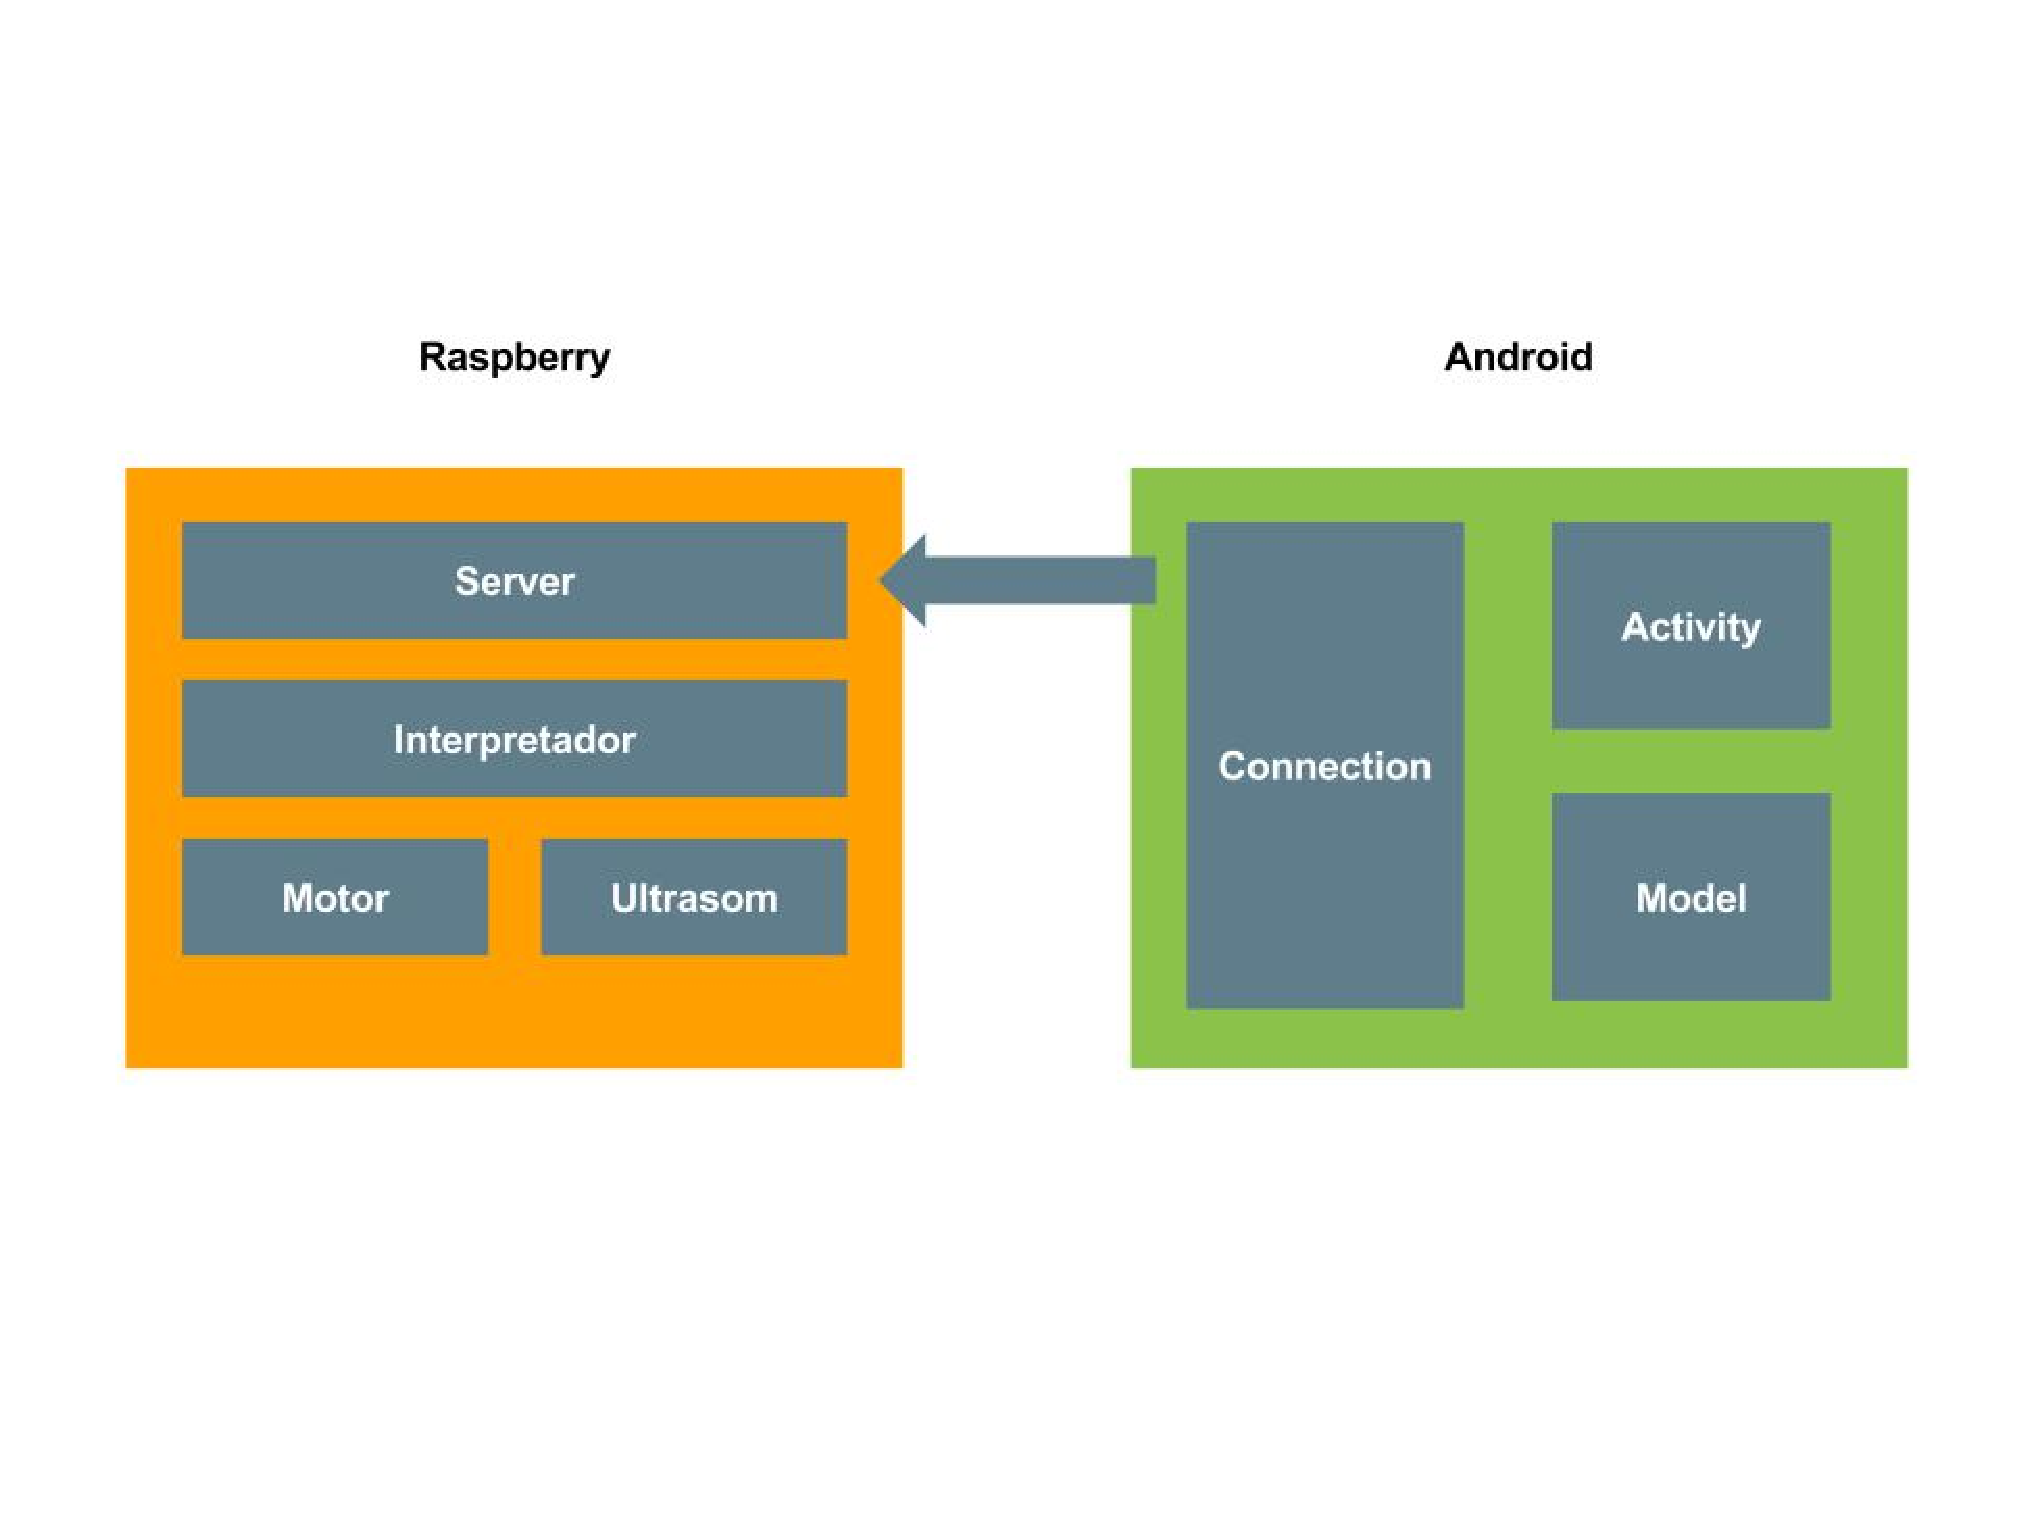
\includegraphics[width=0.7\textwidth]{figuras/overview_down.eps}
    \caption{Visão geral do sistema e a sua comunicação}
    \label{fig:overview_down}
\end{figure}

Uma breve descrição para cada uma dos módulos:
\begin{itemize}
    \item \textbf{Server}: responsável por receber os programas enviados pelo aplicativo Android;
    \item \textbf{Interpretador}: responsável por interpretar os dados contidos no programa recebido;
    \item \textbf{Motor e Ultrassom}: representa os atuadores que executarão os comandos interpretados pelo programa. Ainda existe outros
    possíveis atuadores que poderão ser acoplados ao Rapberry;
    \item \textbf{Connection}: garante a conexão entre o servidor e o aplicativo. Responsável por enviar os programas para o servidor;
    \item \textbf{Activity}: operações de interação com o usuário. Camada de apresentação e coleta de dados do usuário;
    \item \textbf{Model}: modelos representativos da aplicação.
\end{itemize}

A comunicação ocorre por wifi (mais detalhes nas proximas seções), e a execução das instruções são transferida por uma arquivo JSON.
A visão operacional do produto (Figura \ref{fig:overview}) se resume em três passos: \textbf{construção} do programa (JSON), \textbf{transferência}
para o Alfa, \textbf{execução} do programa.

\begin{figure}[H]
    \centering
    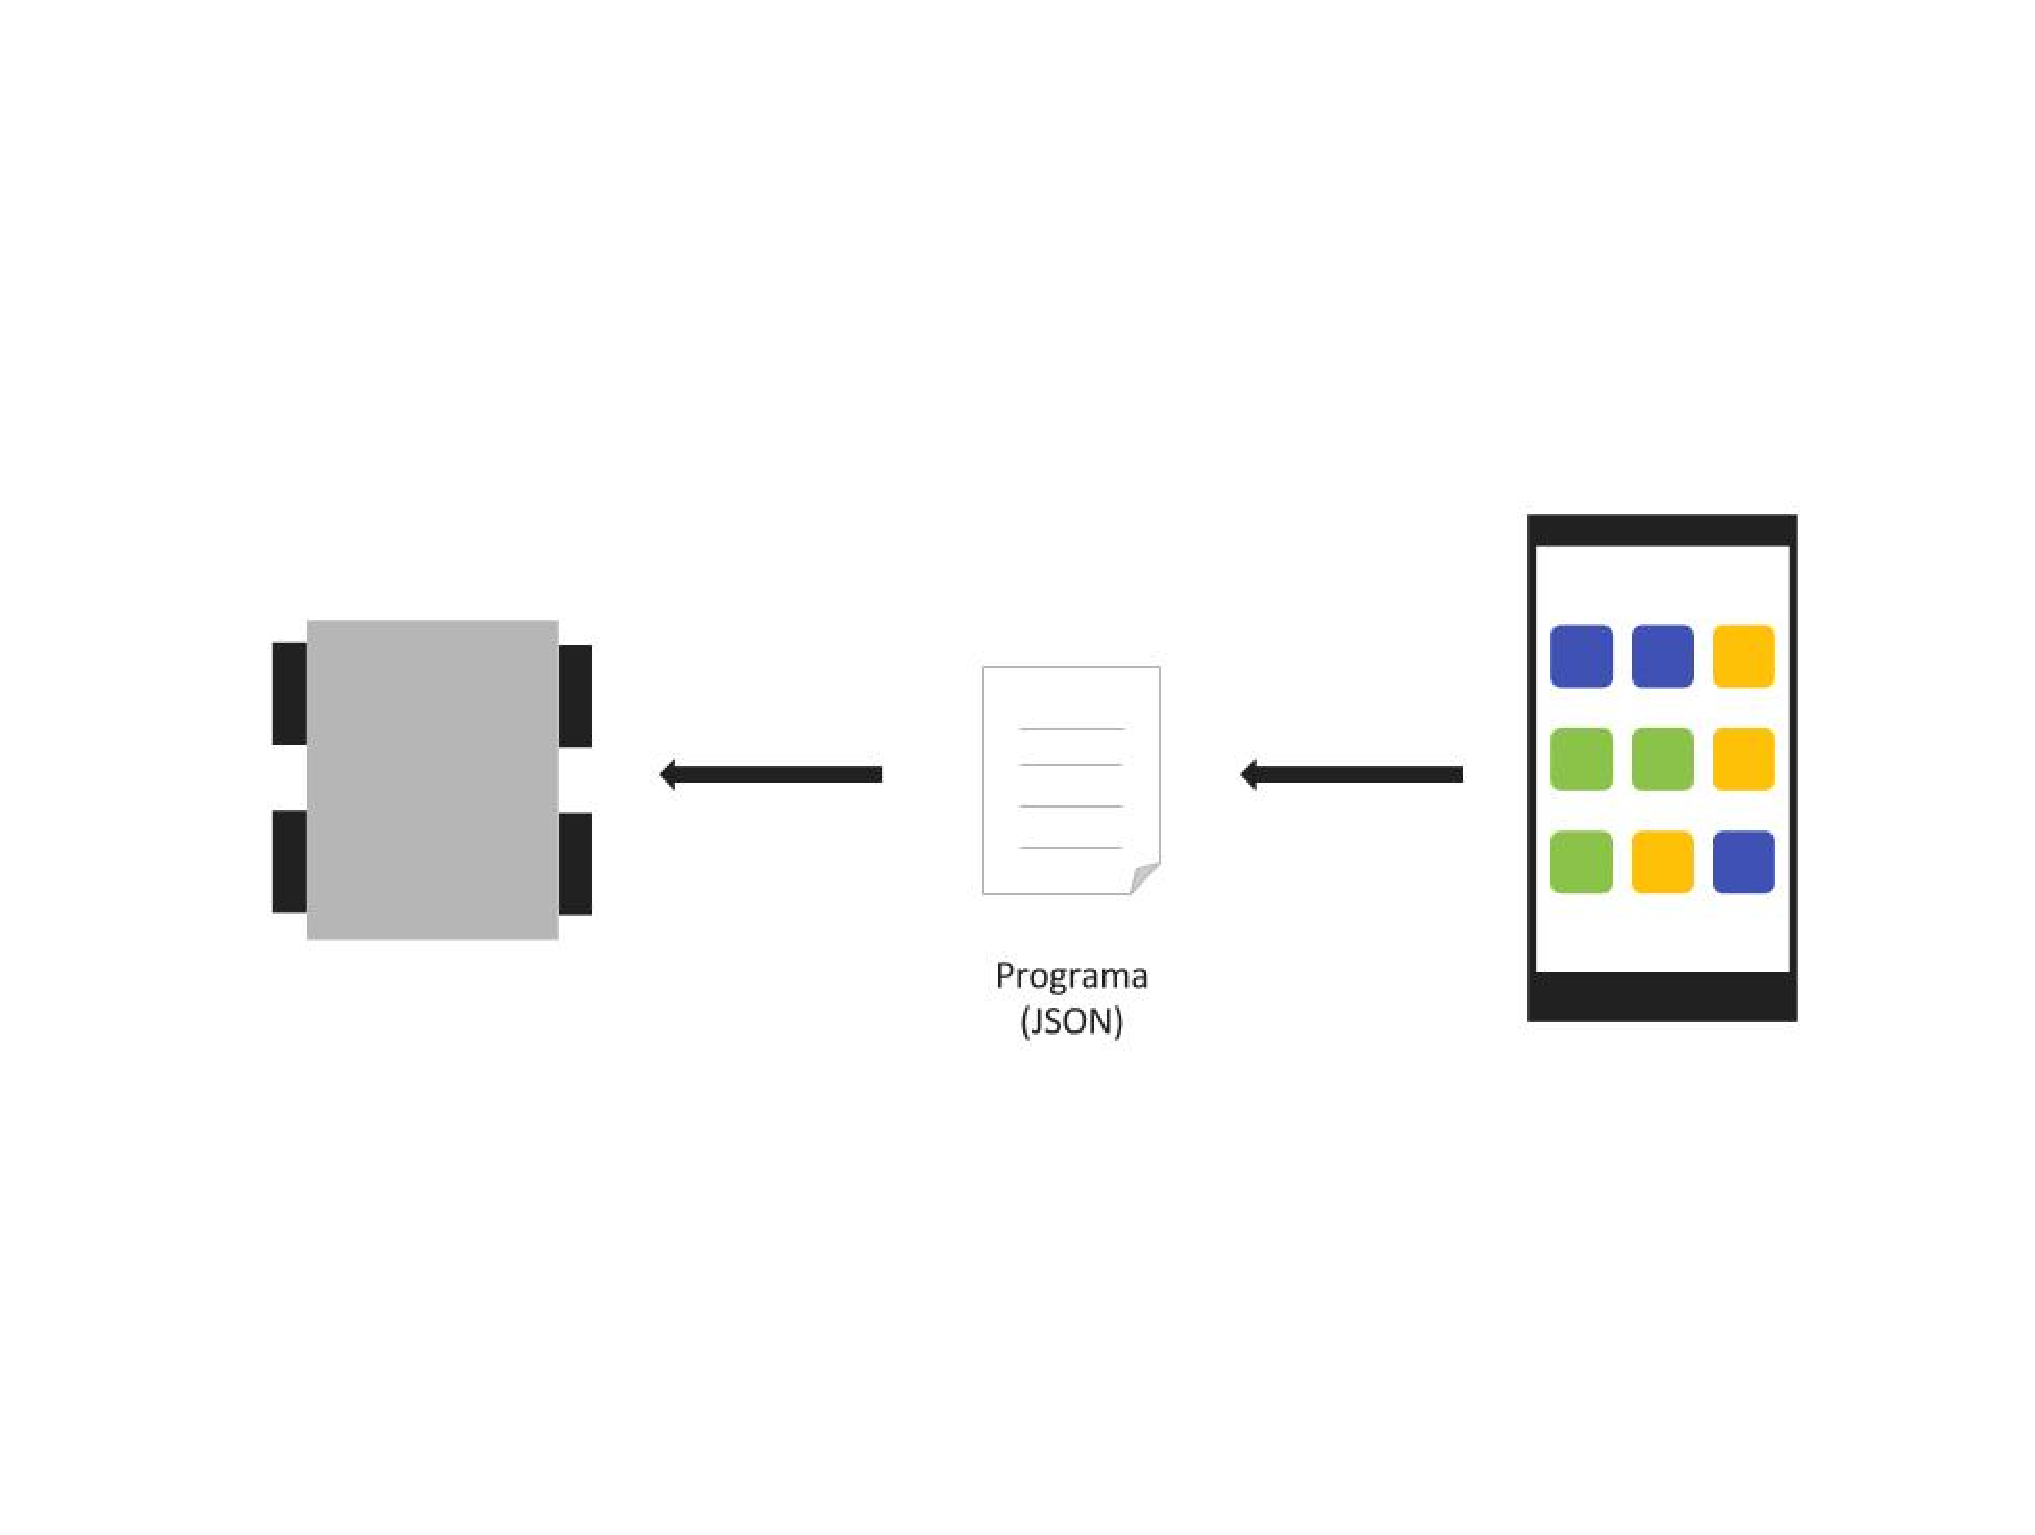
\includegraphics[width=0.7\textwidth]{figuras/overview.eps}
    \caption{Visão operacional do sistema}
    \label{fig:overview}
\end{figure}

As operações descritas na Figura \ref{fig:sequencia} demonstram a forma como as ações serão executadas em forma de diagrama de sequência

\begin{figure}[H]
    \centering
    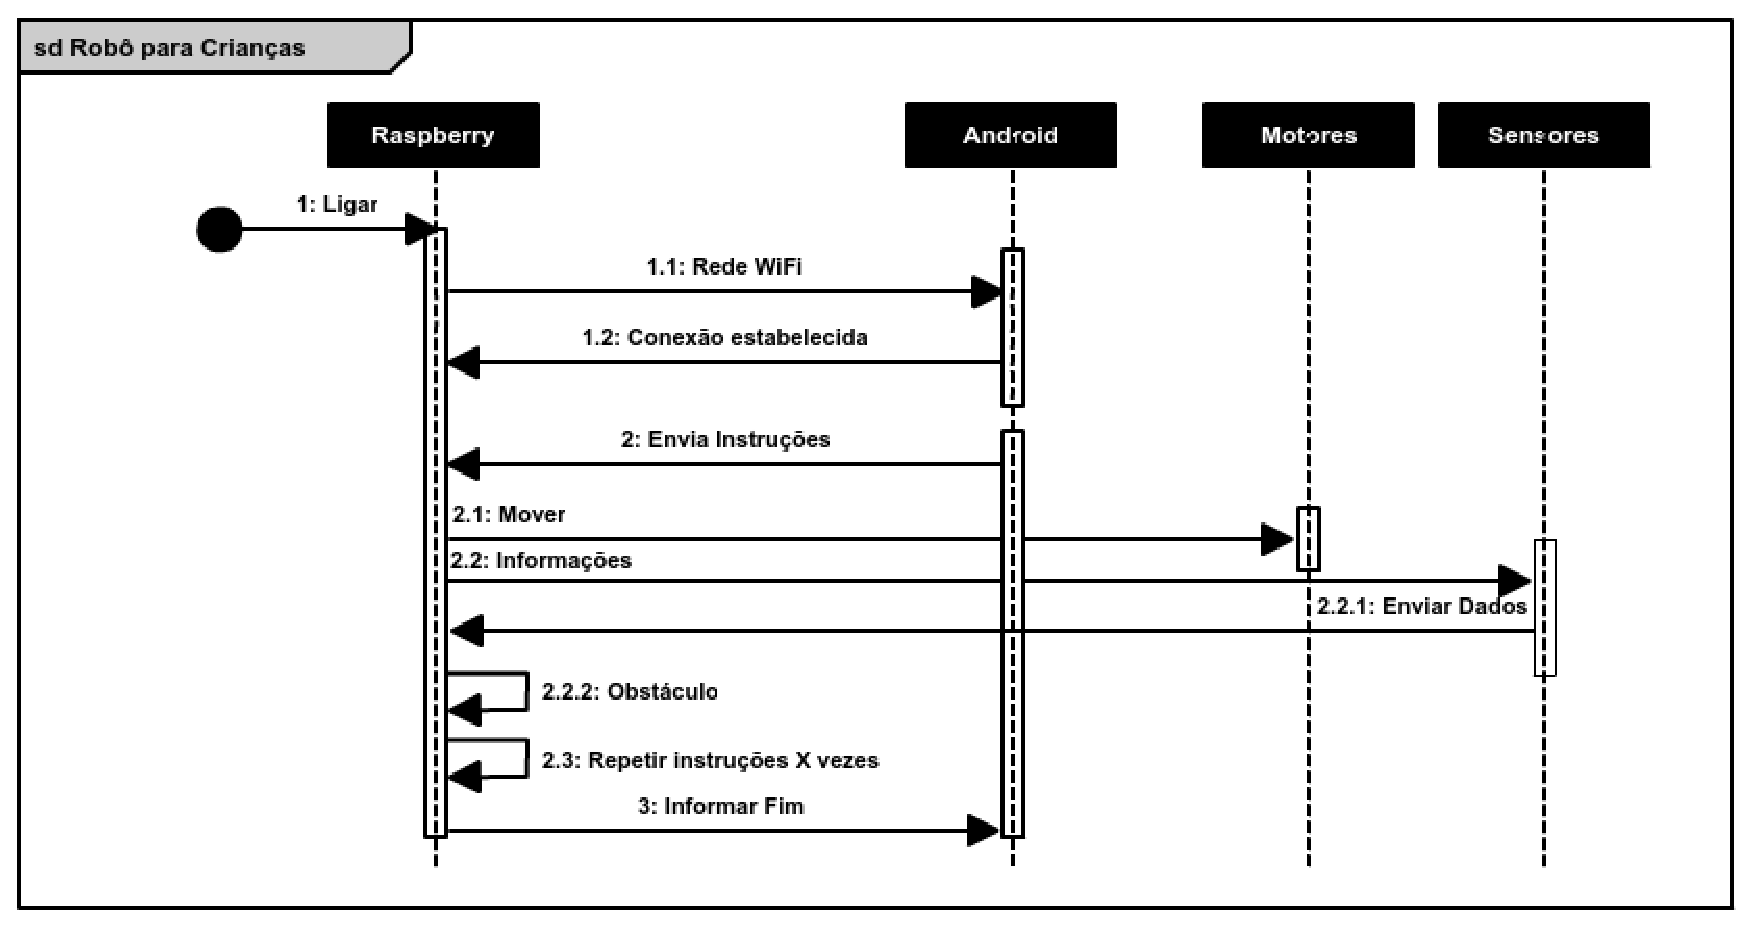
\includegraphics[width=0.8\textwidth]{figuras/diagrama_de_sequencia.eps}
    \caption{Diagrama de sequência - Visão geral dos sistemas}
    \label{fig:sequencia}
\end{figure}

\subsection{Configuração Wi-Fi}

Para o desenvolvimento da comunicação entre o robô educacional e o aplicativo em dispositivos móveis ANDROID escolheu-se a aplicação da
tecnologia de comunicação \textit{Wi-Fi}, de modo que é acoplado ao Raspberry Pi um dongle \textit{Wi-Fi} (adaptador USB que adiciona funcionalidades à
dispositivos, neste caso o adaptador \textit{Wi-Fi} permite interação com este tipo de comunicação) para que se possa configurar propriamente o
Raspberry Pi como um ponto de acesso de rede (Access Point ou Hotspot).

\begin{figure}[H]
    \centering
    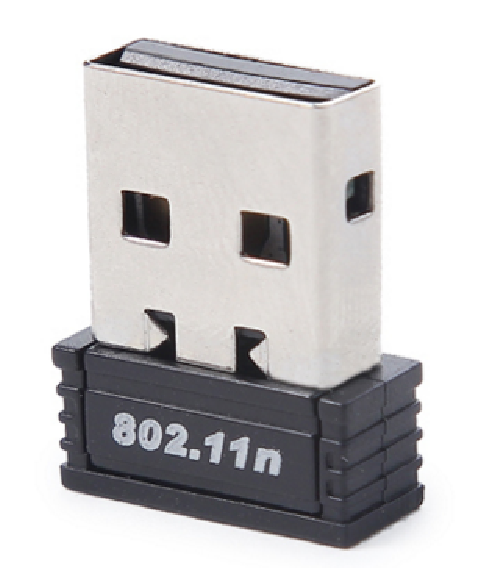
\includegraphics[width=0.4\textwidth]{figuras/adaptador_wifi.eps}
    \caption{WiFi Dongle}
    \label{fig:wireless}
\end{figure}

A tecnologia \textit{Wi-Fi} foi escolhida por apresentar parâmetros que condizem com as necessidades do projeto (largura de banda – aproximadamente
22MHz – condizente com o requerido, alcance de aproximadamente 100 metros, menor latência, maior segurança, taxa de transmissão de bits –
aproximadamente 600 Mbps - satisfatória para o projeto), outras tecnologias como por exemplo bluetooh, ZigBee e UWB não foram utilizadas
por apresentarem características inferiores as desejadas para o projeto, inaplicabilidade ou por capacidade superior a requerida,
respectivamente (IECON). Para a configuração do Raspberry Pi como Access Point instalou-se e configurou-se o protocolo de serviço DHCP
(onde o mesmo utiliza um modelo cliente-servidor, gerenciando automaticamente os endereços de IP, gateway padrão, máscara de sub-rede e
outros parâmetros da conexão dos dispositivos conectados ao access point), bem como instalou-se e configurou-se o Hostapd, que se trata
de um programa no “user-space” que é executado em plano de fundo utilizado que realiza a autenticação de servidores e permite a criação
de pontos de acesso \cite{wireless:2015}, neste caso, para o controle do robô.

\subsection{Sensoriamento}

Em termos de interação com o ambiente na resposta do robô aos comandos fornecidos pela estrutura lógica de blocos do aplicativo,
inicialmente realiza-se o sensoriamento utilizando-se um sensor de ultrassom na análise da distância do robô com relação aos objetos
ao seu redor. Em princípio, implementa-se o sensoriamento de distância utilizando o modelo HC-RS04 que apresenta especificações de
funcionamento (medição de distância de 2cm a 500cm, resolução de 0.3cm, frequência de 40kHz) e alimentação (5V DC) satisfatórias para
a viabilização deste aspecto do projeto \cite{micropik:2015}.

Umas das terminações do sensor de ultrassom emite um pulso de duração de 10 microssegundos (pino trig é ativado), o sinal é 
refletido no objeto mais próximo e retorna para a segunda terminação onde aciona um de seus pinos (echo) sinalizando a chegada do sinal,
o período de resposta (processamento) do sensor é igual a 50ms o que não leva a atrasos a serem considerados neste projeto.

\begin{figure}[H]
    \centering
    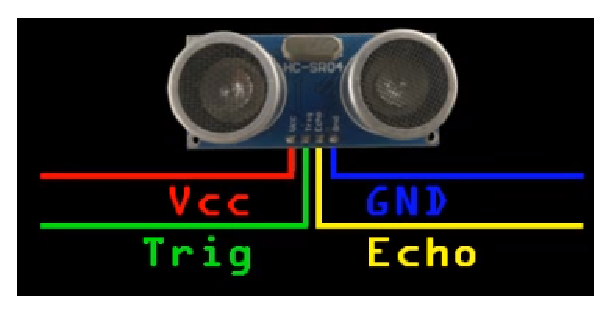
\includegraphics[width=0.5\textwidth]{figuras/pinos_ultrassom.eps}
    \caption{Sensor de Ultrassom HC-RS04 e respectivos pinos.}
    \label{fig:pinos_ultrassom}
\end{figure}

No que diz respeito a programação deste sensor é importante ressaltar que se deve considerar que o pulso emitido pelo sensor percorre
duas vezes a distância entre o robô e o objeto, desta forma deve-se considerar a seguinte fórmula (levando-se em consideração a velocidade
do som igual a 340m/s):

\begin{figure}[H]
    \centering
    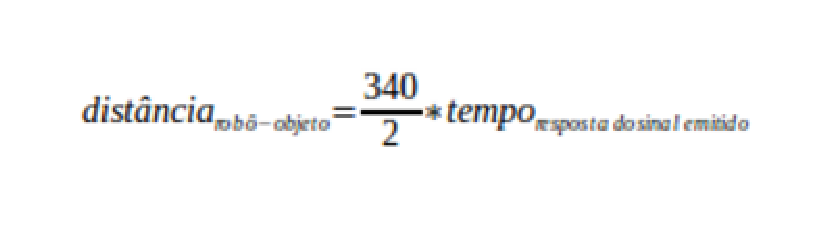
\includegraphics[width=0.6\textwidth]{figuras/distancia.eps}
    \caption{(1)}
    \label{fig:distancia_sensor}
\end{figure}

Para implementação do sensor de ultrassom HC-RS04 deve-se considerar um divisor de tensão para o pino echo uma vez que este pino
trabalha com uma tensão igual a 3.3V. Dessa maneira considerando um resistor (que também atua como um resistor e pull-down), tem-se:

\begin{figure}[H]
    \centering
    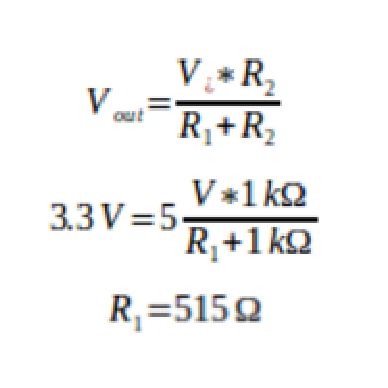
\includegraphics[width=0.3\textwidth]{figuras/vout.eps}
    \caption{(2)}
    \label{fig:vout}
\end{figure}

Dessa maneira utilizou-se um valor comercial disponível mais próximo igual a 680ohms. Pode-se observar o esquemático relativo à
implementação do sensor de ultrassom a seguir:

\begin{figure}[H]
    \centering
    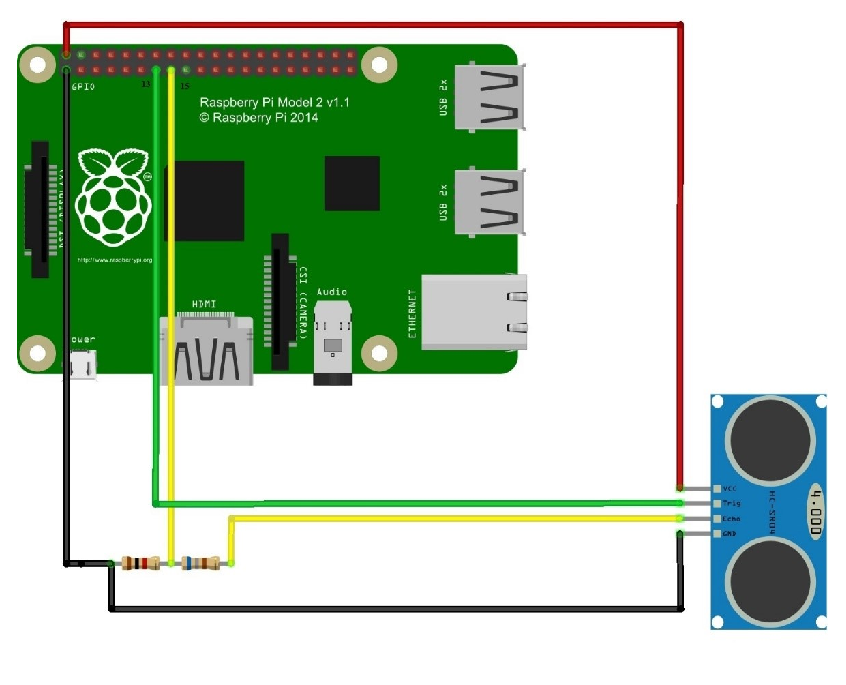
\includegraphics[width=0.8\textwidth]{figuras/esquematico_ultrassom.eps}
    \caption{Esquemático do circuito de implementação do sensor de ultrassom}
    \label{fig:esquematico_ultrassom}
\end{figure}

O código referente à programação do sensor de distância ultrassom, em linguagem Python, está em Apêndice a este relatório.

\subsection{Comunicação Robô-Aplicativo}

A comunicação entre o robô e o aplicativo mobile foi realizada através de uma comunicação do tipo Cliente/Servidor utilizando a
API de Sockets em Python, onde o servidor foi implementado no Raspberry PI, e o cliente foi configurado no aplicativo. Foi utilizado
o protocolo TCP/IP na realização da comunicação, esse protocolo foi utilizado por ser atualmente o mais completo e aceito protocolo
disponível, além de todos os sistemas operacionais modernos oferecerem suporte para o mesmo. Além disso, o protocolo TCP/IP é do tipo 
textit{stream}, o que estabelece algumas características de transmissão, como confiabilidade, ordem, controle de fluxo e bidirecionalidade.
A seguir tem-se um diagrama ilustrando as funções utilizadas na implementação da comunicação cliente servidor utilizando o protocolo TCP/IP:

\begin{figure}[H]
    \centering
    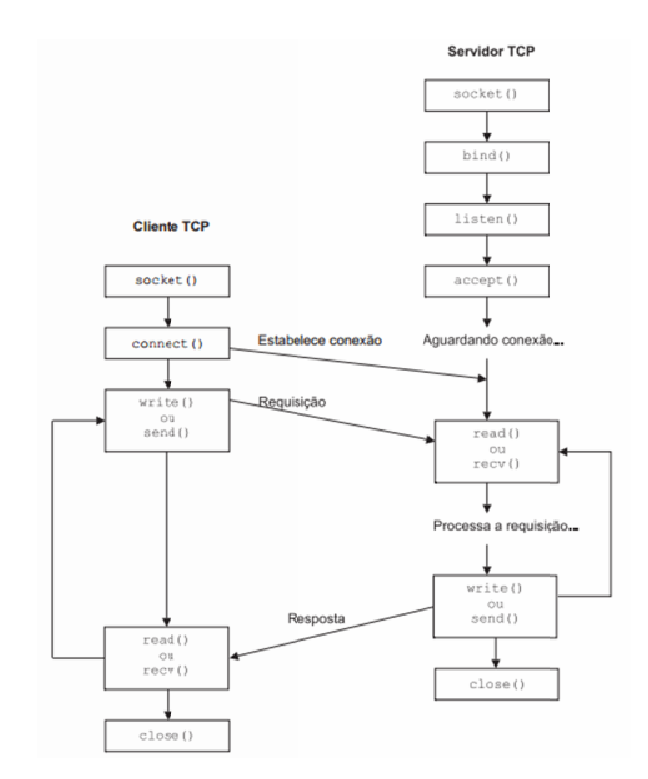
\includegraphics[width=0.8\textwidth]{figuras/diagrama_socket.eps}
    \caption{Diagrama de blocos do Sistema Cliente/Servidor utilizando TCP/IP}
    \label{fig:diagrama_socket}
\end{figure}

\subsection{Execução dos Blocos Lógicos}

As tarefas a serem executadas pelo robô são enviadas através de um arquivo do tipo JSON (Java Script Object Notation), onde o mesmo é
recebido pelo servidor através da comunicação via sockets e interpretado a fim de executar as solicitações do usuário através da lógica
de blocos. Para isso são passadas as chamadas das funções referentes a cada bloco lógico através do arquivo JSON, onde essas funções são
lidas e interpretadas no Raspberry PI, com o intuito de ativar e controlar os motores do robô de acordo com as tarefas referentes a cada
bloco lógico.

Os motores do robô são acionados e controlados utilizando 4 pinos GPIO do Raspberry PI e uma Ponte H. De modo que o Raspberry PI é responsável
por enviar sinais PWM (configurados utilizando funções em python) para a Ponte H, referentes a velocidade e a direção que se deseja passar ao
robô na execução de determinado bloco lógico. A Ponte H é responsável por inverter o sentido de rotação dos motores quando necessário, e
também por sincronizar a inicialização e rotação dos mesmos.

\subsection{Ponte H}

A ponte H é um circuito designado para controlar o sentido e a velocidade dos motores DC do robô. Por ser um circuito do tipo chopper E,
o mesmo circuito converte corrente contínua fixa em uma tensão de corrente contínua variável. Dessa forma, pode-se determinar o sentido da
corrente e a polaridade da tensão. A ponte H é feita de componentes como Switches, Relays e Mosfets.

A figura abaixo mostra uma ponte H módulo L298N que foi utilizada no projeto. Este dispositivo foi utilizado considerando sua versatilidade
e simplicidade de implementação, além de sua funcionalidade, como o controle de vários motores simultaneamente. Uma outra vantagem é o fato
do L298N poder controlar as altas correntes dos motores, ela literalmente faz uma ‘ponte’ entre as correntes baixas do circuito lógico do
Raspberry PI e dos motores DC utilizados para movimentar as rodas. As especificações do módulo L298N encontram-se abaixo:

\begin{itemize}
    \item I. Chip: L298N
    \item II. Tensão Lógica: 5V
    \item III. Corrente Lógica: 0 mA - 36 mA
    \item IV. Temperatura de funcionamento: -20 C a +135 C
    \item V. Drive Voltage: 5V-35V
    \item VI. Drive current: 2A (MAX para uma ponte H)
    \item VII. Máxima Potência: 25W
    \item VIII. Dimensão: 43x43x27mm
\end{itemize}

\begin{figure}[H]
    \centering
    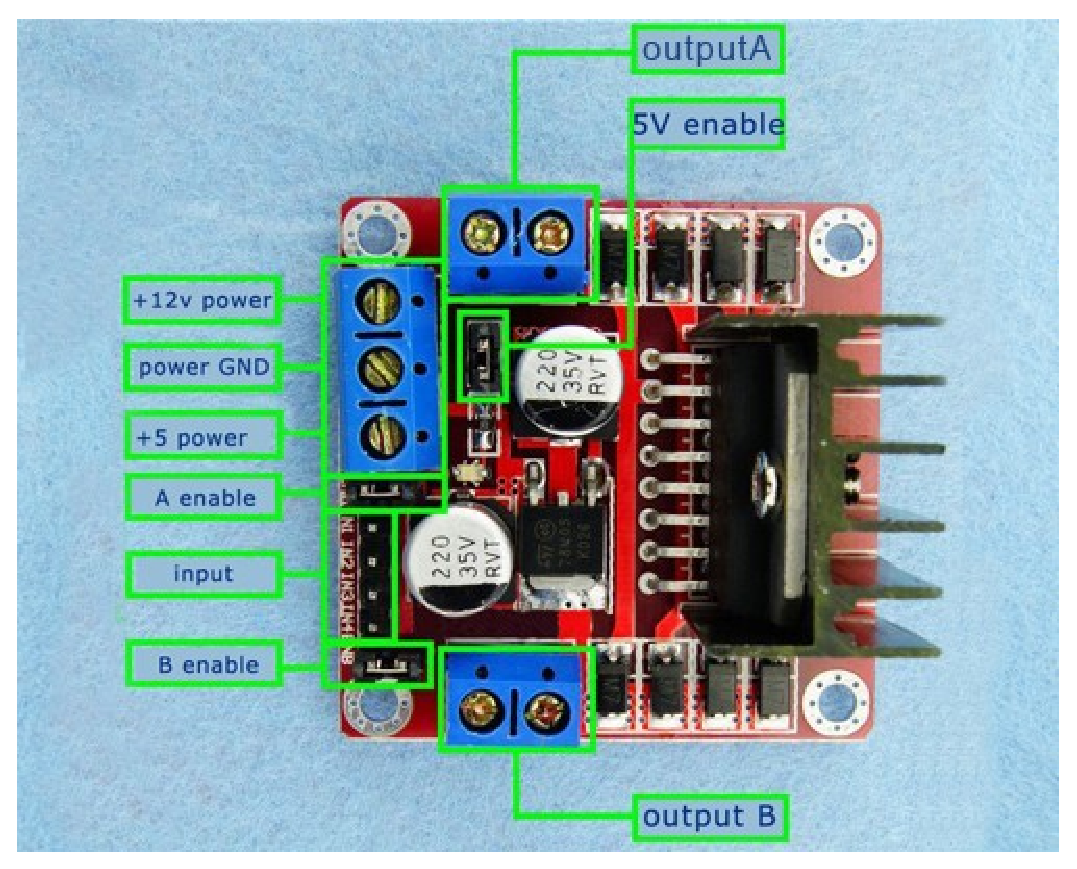
\includegraphics[width=0.8\textwidth]{figuras/ponteH.eps}
    \caption{Ponte H L298N e seus terminais. Fonte: Proesi - Componentes Eletrônicos}
    \label{fig:ponteH}
\end{figure}

A conexão com o Raspberry Pi e os motores pode ser demonstrado pela figura \ref{fig:esquematico_componentes}. O terra do L298N é comum com o
Raspberry, todavia necessita de uma alimentação externa, no caso 9V. Escolhe-se quatro pinos para serem ligados da ponte H ao Raspberry Pi,
os mesmo pinos são definidos como saída no código, a figura \ref{fig:esquematico_componentes} ilustra a conexão de apenas dois pinos que saem
da ponte H e fazem a conexão no Raspberry Pi. Controlam-se as velocidades dos motores definindo a frequência do PWM e através do duty cycle
é definido a porcentagem do tempo total que os motores estão na posição de trabalho. Utilizando a tabela \ref{fig:tabela_ponte_H_2} como
referência, é possível definir o sentido dos motores e sua ação colocando os pinos em HIGH ou LOW  dependendo da fonte da alimentação. 

\begin{figure}[H]
    \centering
    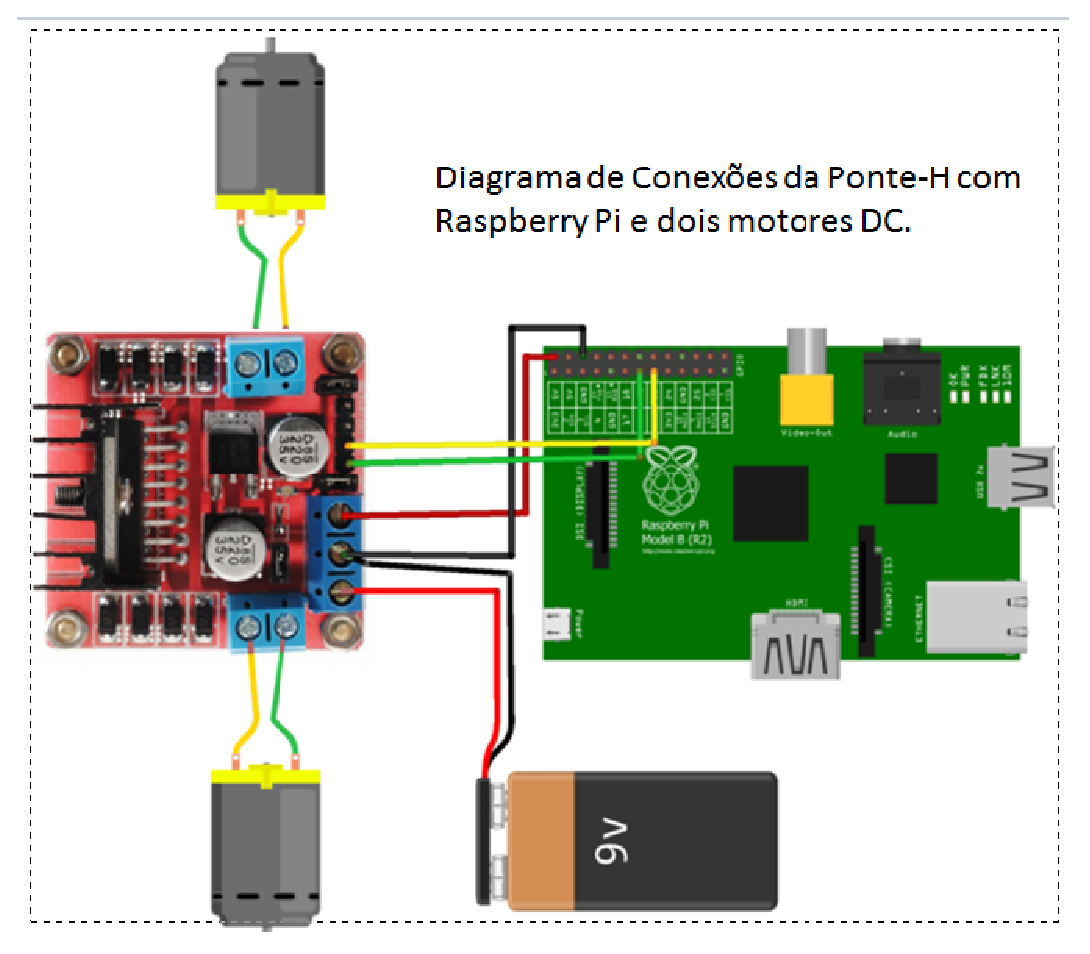
\includegraphics[width=0.8\textwidth]{figuras/esquematico_componentes.eps}
    \caption{Diagrama de conexões da Ponte H com periféricos.}
    \label{fig:esquematico_componentes}
\end{figure}

\begin{figure}[H]
    \centering
    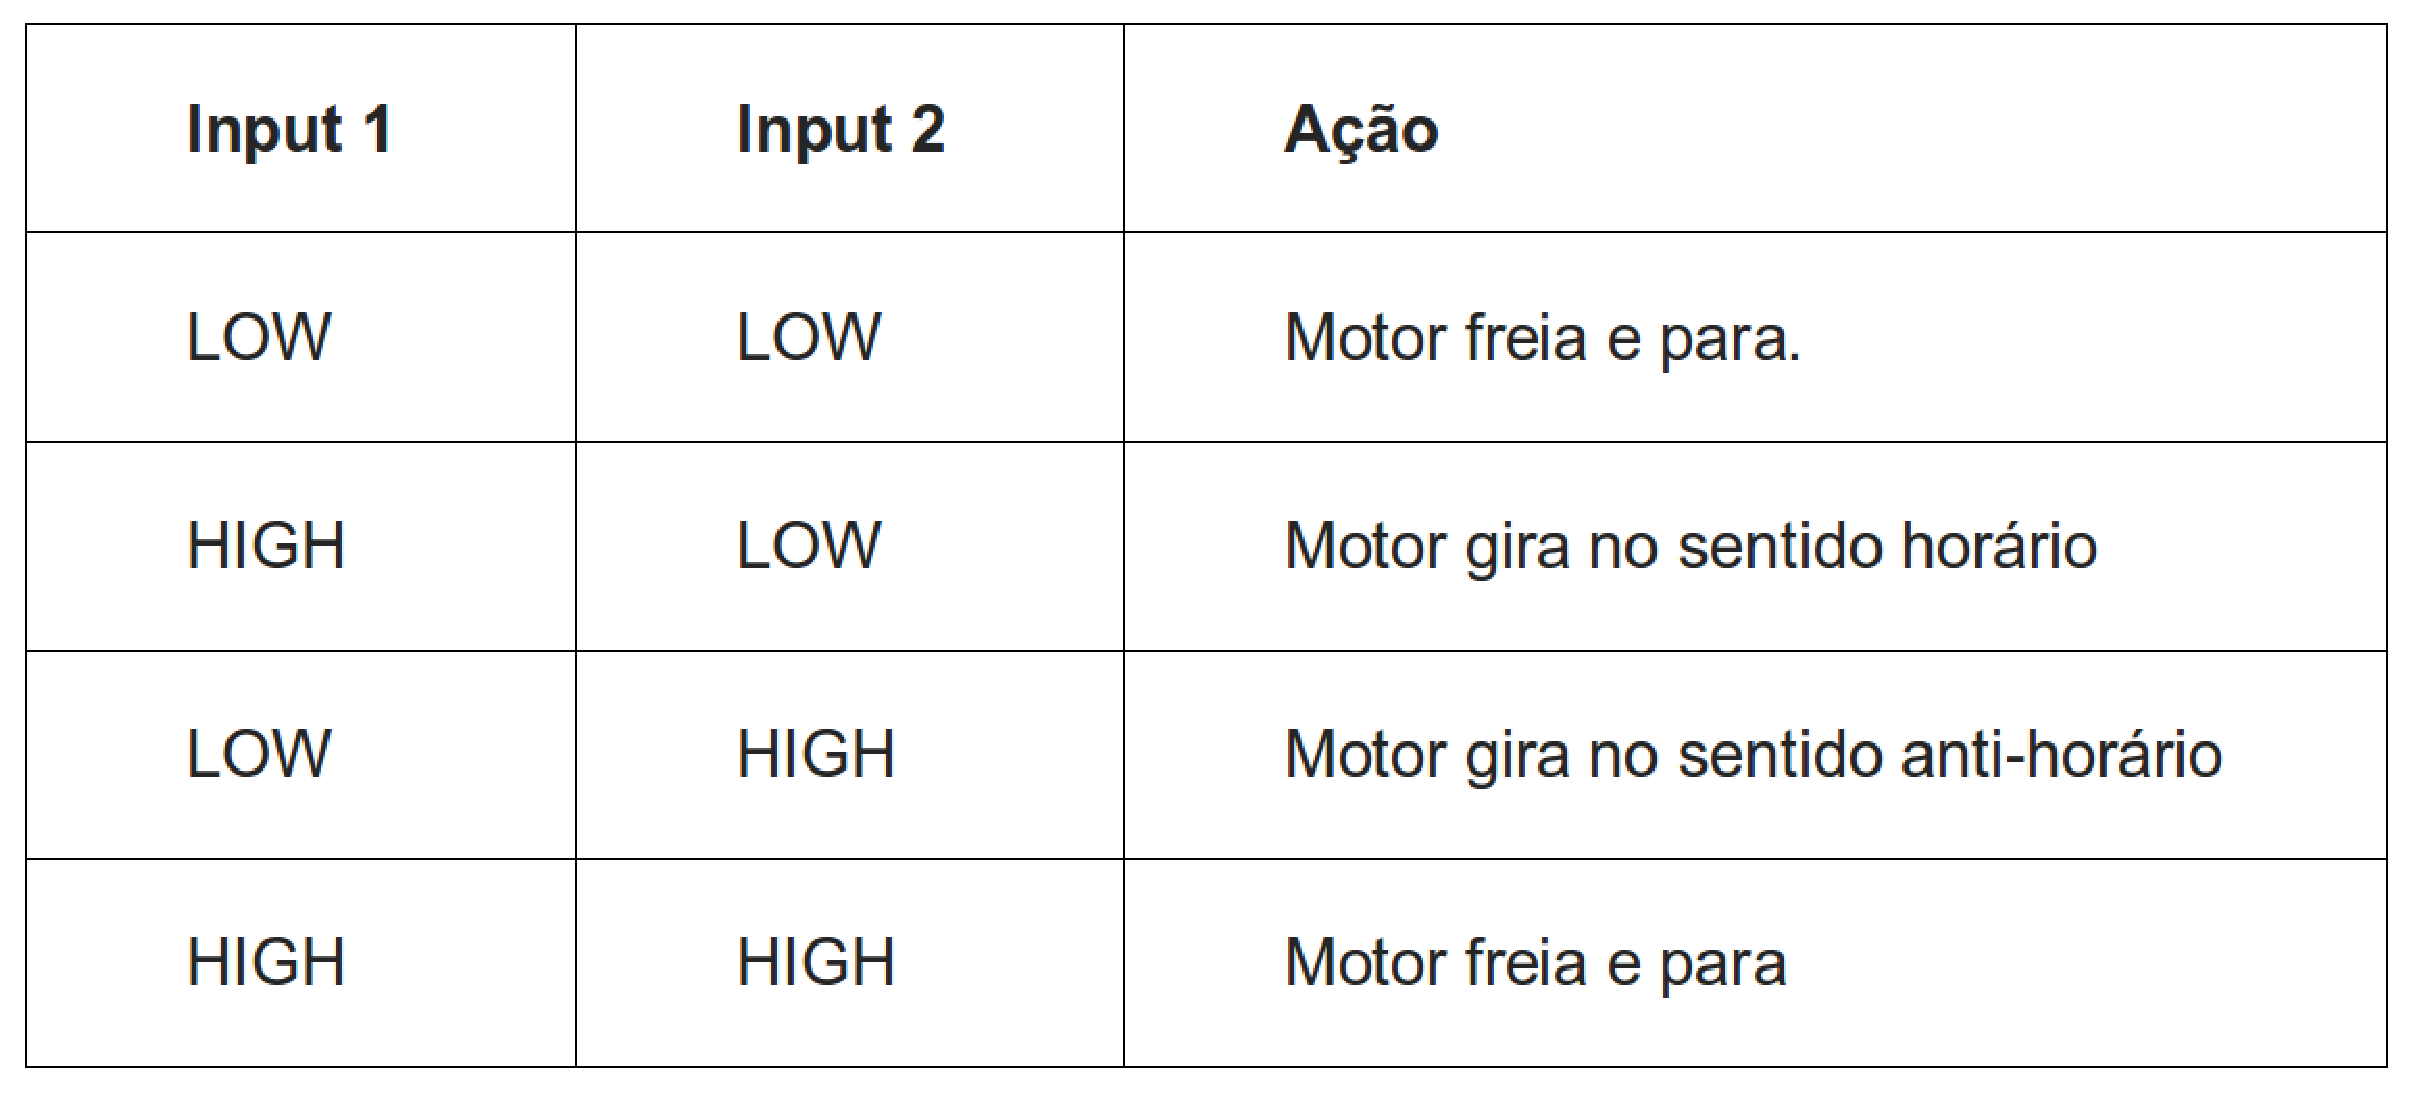
\includegraphics[width=0.8\textwidth]{figuras/tabela_ponte_H_2.eps}
    \caption{Tabela verdade utilizada no módulo Ponte H - Motor}
    \label{fig:tabela_ponte_H_2}
\end{figure}

\subsubsection{Alimentação da Ponte-H}

Para a alimentação da ponte H propõe-se duas possíveis aplicações, a primeira proposta é a de um elevador de tensão, de tal forma que
elevasse a tensão de saída da bateria utilizada (5 Volts) para 12 V (que é a tensão desejada para a alimentação da ponte H). Dessa maneira,
implementou-se um circuito como o demonstrado na Figura \ref{fig:elevador}, a partir de um circuito integrado elevador de tensão DC-DC MC34063, este
circuito integrado apresenta uma vasta faixa de operação de tensão de entrada (de 3V a 40V), apresenta frequência de operação de 100 kHz,
apresenta baixa corrente de standby, além de fornecer um máximo de até 1.5A de corrente de saída (o que é suficiente para o controle
do motores através da ponte H)\cite{kuhl:2013}.

\begin{figure}[H]
    \centering
    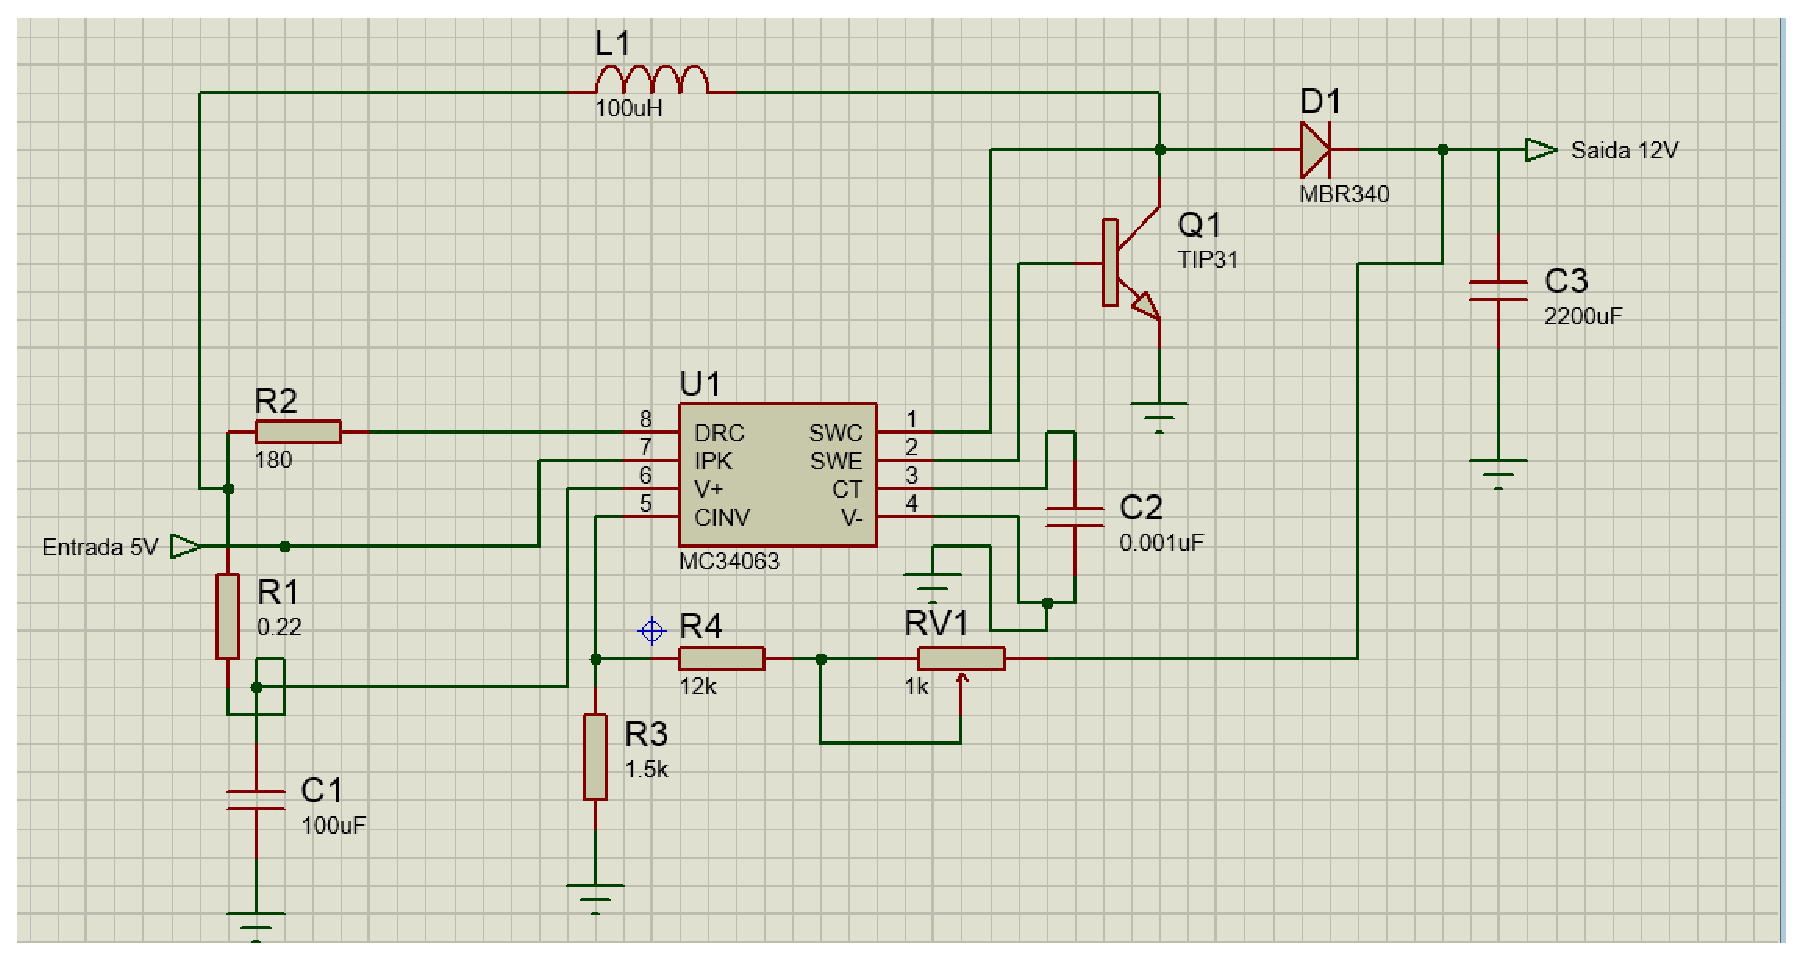
\includegraphics[width=0.9\textwidth]{figuras/elevador.eps}
    \caption{Circuito Elevador de Tensão Implementando-se o MC34063.}
    \label{fig:elevador}
\end{figure}

Os componentes dos circuitos foram escolhidos de maneira a satisfazer os parâmetros de alimentação desejados para a ponte H
 \cite{kuhl:2013}. É importante ressaltar alguns aspectos deste circuito: os resistores são responsáveis pelo valor
de tensão obtido na saída de modo a regular-se  a obter a tensão de saída desejada, o diodo utilizado é do tipo \textit{Schottky Barrier} (por
apresentar baixa queda tensão e rápida resposta de transição entre polarização direta e inversa), utilizou-se um indutor toroidal de
núcleo de ferrite por apresentar características como baixos níveis de perda e estabilidade em níveis altos de temperatura.
Uma segunda proposta é a de um regulador de tensão de 12V para uma entrada de alimentação de duas baterias de 9V em série (que resultariam
em 18V). Então, nesta proposta o principal elemento para implementação é um regulador de tensão LM7812, aplicado juntamente a alguns
capacitores (utilizados como filtros de possíveis ripples no sinal)e um diodo de proteção, como demonstrado na Figura \ref{fig:regulador}.

\begin{figure}[H]
    \centering
    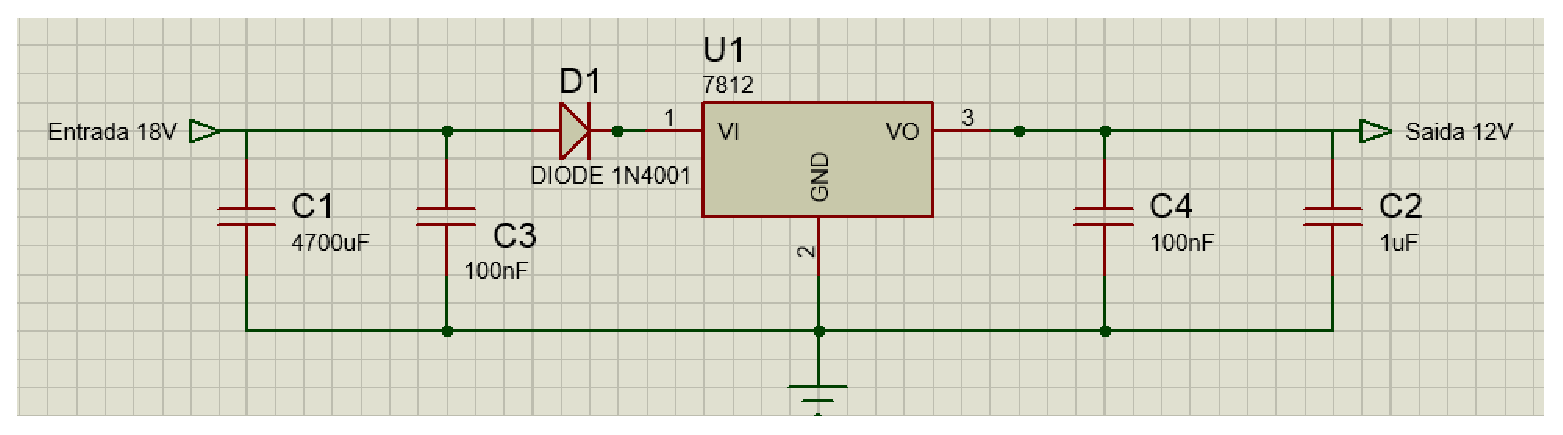
\includegraphics[width=0.9\textwidth]{figuras/regulador.eps}
    \caption{Circuito Regulador de Tensão Implementando-se LM7812.}
    \label{fig:regulador}
\end{figure}

Tendo em vista o design do produto implementou-se LEDs do tipo RGB (vermelho, verde e azul do inglês red, green and blue) de tal forma
que os LEDs assumam a cor que diz respeito a cor do bloco escolhido no aplicativo para o controle, a  Figura 3.2.5c apresenta a estrutura
de LED do tipo RGB (que basicamente se comporta como três LEDs com cátodo em comum). Sendo assim, cada um dos ânodos dos LEDs são
conectados a um pino diferente do Raspberry Pi para que se controle individualmente cada uma das cores.

Considerando uma corrente de limiar de 4mA para alimentar o LED e uma queda de tensão de 1.89V, 2.65V e 2.83V para os LEDs vermelho,
verde e azul (respectivamente) utiliza-se equivalências de resistores de 330ohm em paralelo para a queda de tensão em cada uma das resistências
equivalentes (a queda de tensão em cada uma das cores do LED RGB somada a queda de tensão sobre a resistência conectada ao seu ânodo deve
ser aproximadamente igual a 3.3V, que é a tensão de alimentação no cátodo comum) , é importante mencionar que para
que se use cada uma das cores deve-se configurar o pino no Raspberry Pi correspondente a cor desejada para nível lógico “baixo” (ou 0
Volts) permitindo a polarização positiva, e ainda ressalta-se que serão implementados três LEDs RGB para intensificar o brilho e as cores.

\begin{figure}[H]
    \centering
    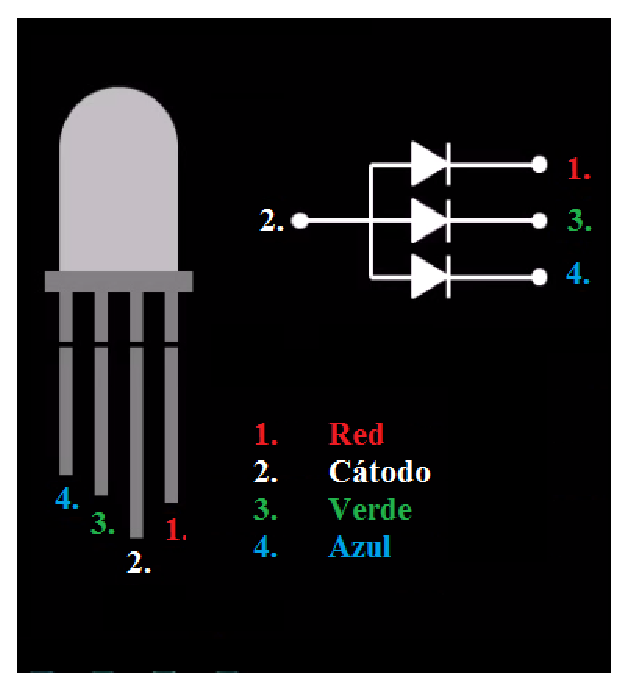
\includegraphics[width=0.4\textwidth]{figuras/led.eps}
    \caption{Estrutura Led RGB Cátodo Comum.}
    \label{fig:led}
\end{figure}

\begin{figure}[H]
    \centering
    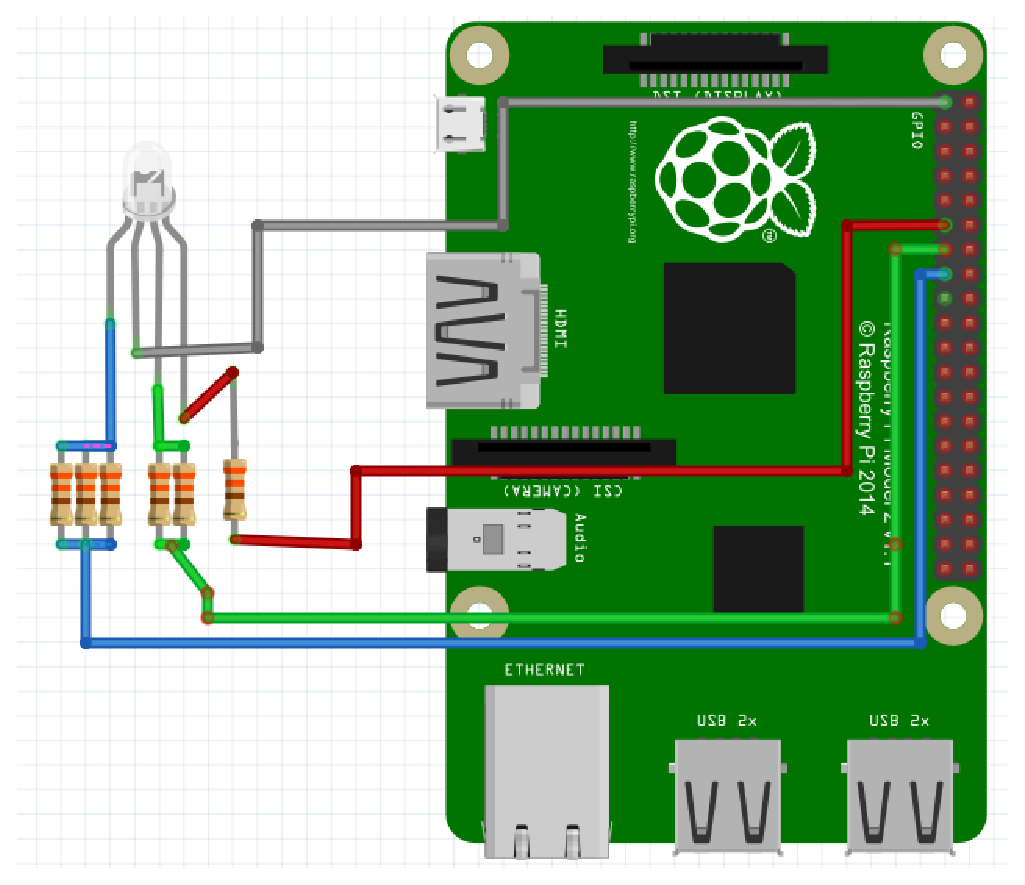
\includegraphics[width=0.5\textwidth]{figuras/esquematico_led.eps}
    \caption{Esquemático Geral das Ligações para um LED RGB.}
    \label{fig:esquematico_led}
\end{figure}

Como para a implementação do sensor de ultrassom, também desenvolveu-se um código de programação para o controle dos LEDs, o código
em Python está em apêndice a este documento com o título (Apêndice B). Os datasheets utilizados na confexão dos circuitos estão em anexo.


\subsection{Aplicativo}

O aplicativo de controle do robô será implementado para o sistema operacional Android usando a linguagem de programação Java. A versão mínima do
SDK será a 8 e a versão alvo será a 23. Por tanto as versões do SO suportadas serão da 2.2 (\textit{Froyo}) até a 6.0 (\textit{Marshmallow}).

Os métodos que merecem destaque são \textit{MyTouchListener()} e a função de criação e envio das instruções:
\begin{itemize}
\item MyTouchListener(): responsável pelo monitoramento dos toques na tela do usuário. Implementada a partir da interface View.OnTouchListener
\item Função de criação e envio das instruções: após o usuário ordenar as instruções para o robô, essa função irá criar um arquivo JSON e enviar as instruções pela conexão WiFi via Socket.
\end{itemize}

As instruções estarão em arquivo JSON, criado no código Java a partir do JSONObject. Um exemplo de arquivo com as instruções é mostrado no coódigo abaixo:

\lstinputlisting{code/instruction.json}

Os dados que esse arquivo irá enviar ao Raspberry Pi serão:
\begin{itemize}
	\item Comando/instrução: comando ou instrução para o robô, por exemplo vire a direita.
\end{itemize}

Dentro de cada comando/instrução os seguintes campos estão presentes:
\begin{itemize}
\item Position: posição em que determinada instrução está em todo o conjunto de blocos de instruções
\item Duration: no caso de “mover para frente”, será passada o tempo desse movimento. Cada tempo já é determinado: 1, 2, 5, 10. Cada uma dessas instruções será um bloco diferente na interface do aplicativo
\item Degree: são os graus com que o robô irá virar, caso seja necessário (ainda em avaliação).
\item Power: informação ainda em avaliação se será necessária para o robô, dado que todo o sistema de hardware e mecânico já está definido e não cabe ao aplicativo informar quanto de potência que o motor ou sensor deve ter.
\end{itemize}

Os outros blocos de instrução desejáveis na aplicação, a saber o de obstáculo para introdução do conceito das estruturas de condição e os círculos para introduzir os conceitos de laços de repetição ainda estão em desenvolvimento.

\subsubsection{Prototipação}

Em vista da questão de atratividade do aplicativo para despertar interesse nas crianças, a interfece gráfica do aplicativo contém elementos
coloridos e com uma distribuição mais simples possível para realizar as operações. Com isso foi realizado práticas de prototipação para construção
de um modelo de interação.

\begin{figure}[H]
    \centering
    
\includegraphics[width=0.3\textwidth]{figuras/splash_screen.eps}
    \caption{\textit{Splash Screen} - Tela de Abertura do Aplicativo.}
    \label{fig:splash_screen}
\end{figure}

\begin{figure}[H]
    \centering
    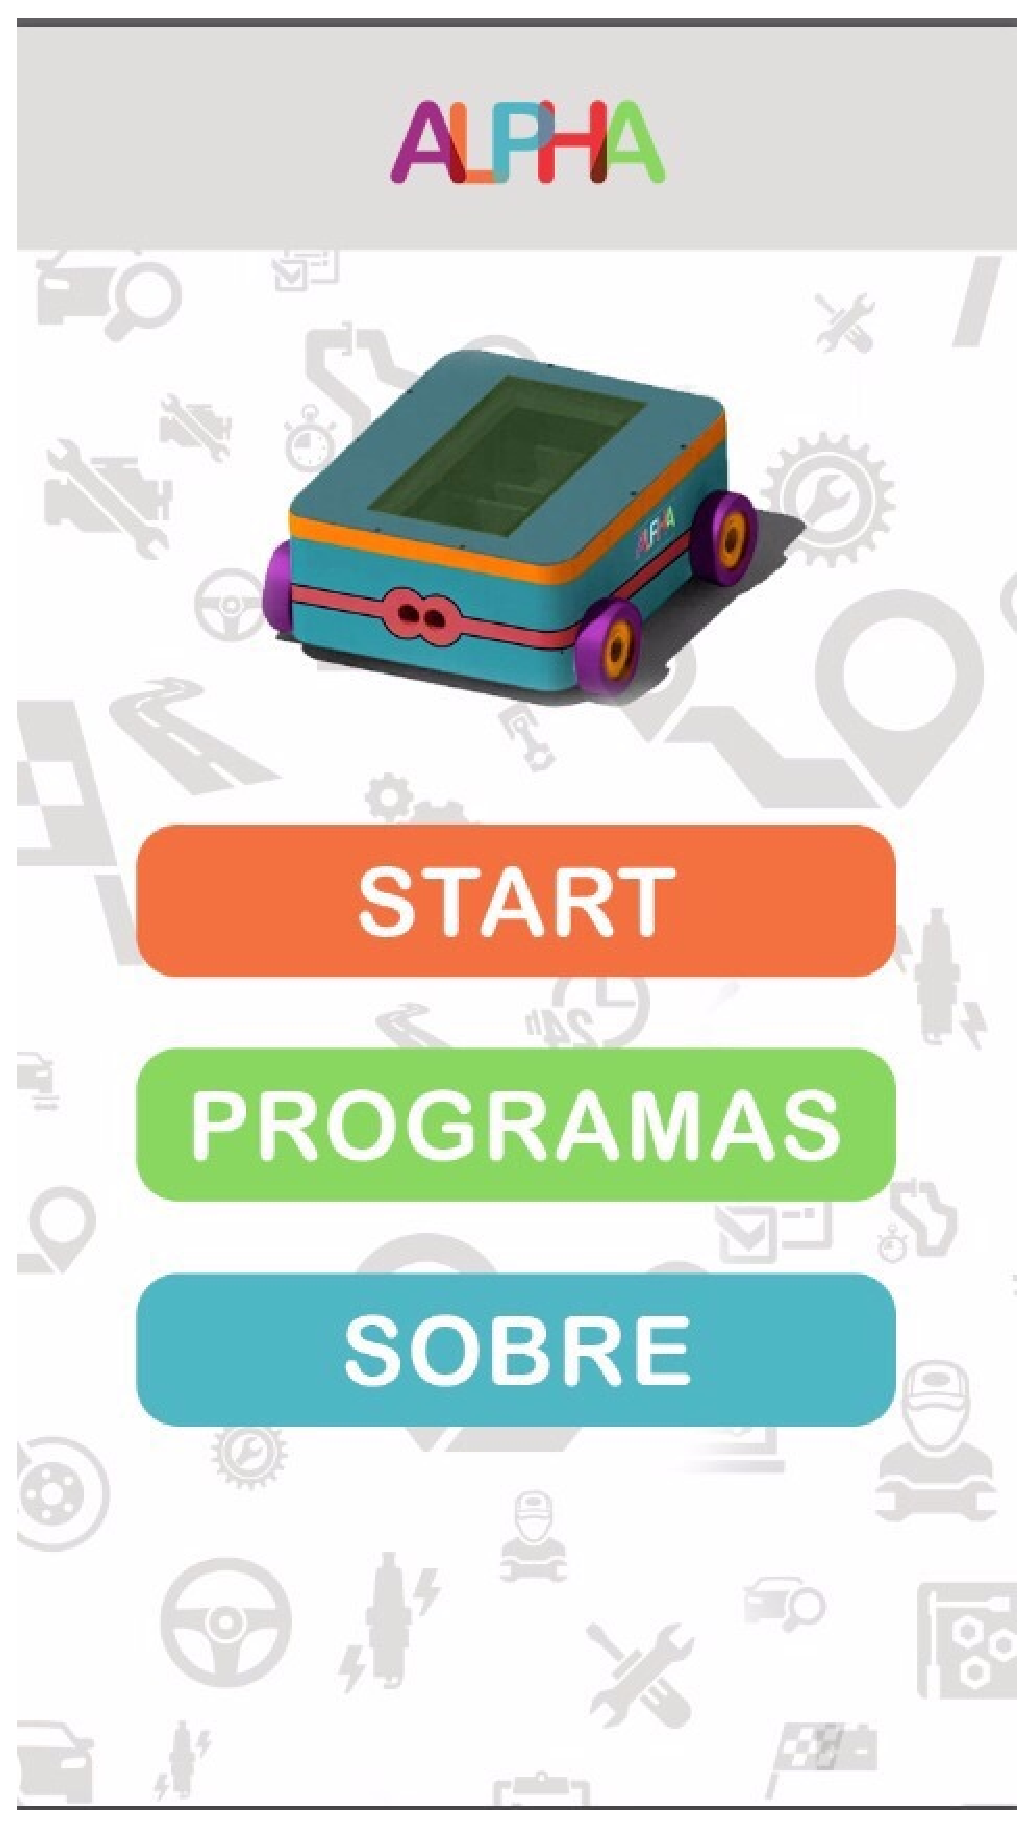
\includegraphics[width=0.3\textwidth]{figuras/main_menu.eps}
    \caption{Tela Principal - \textit{Menu}.}
    \label{fig:main_menu}
\end{figure}

\begin{figure}[H]
    \centering
    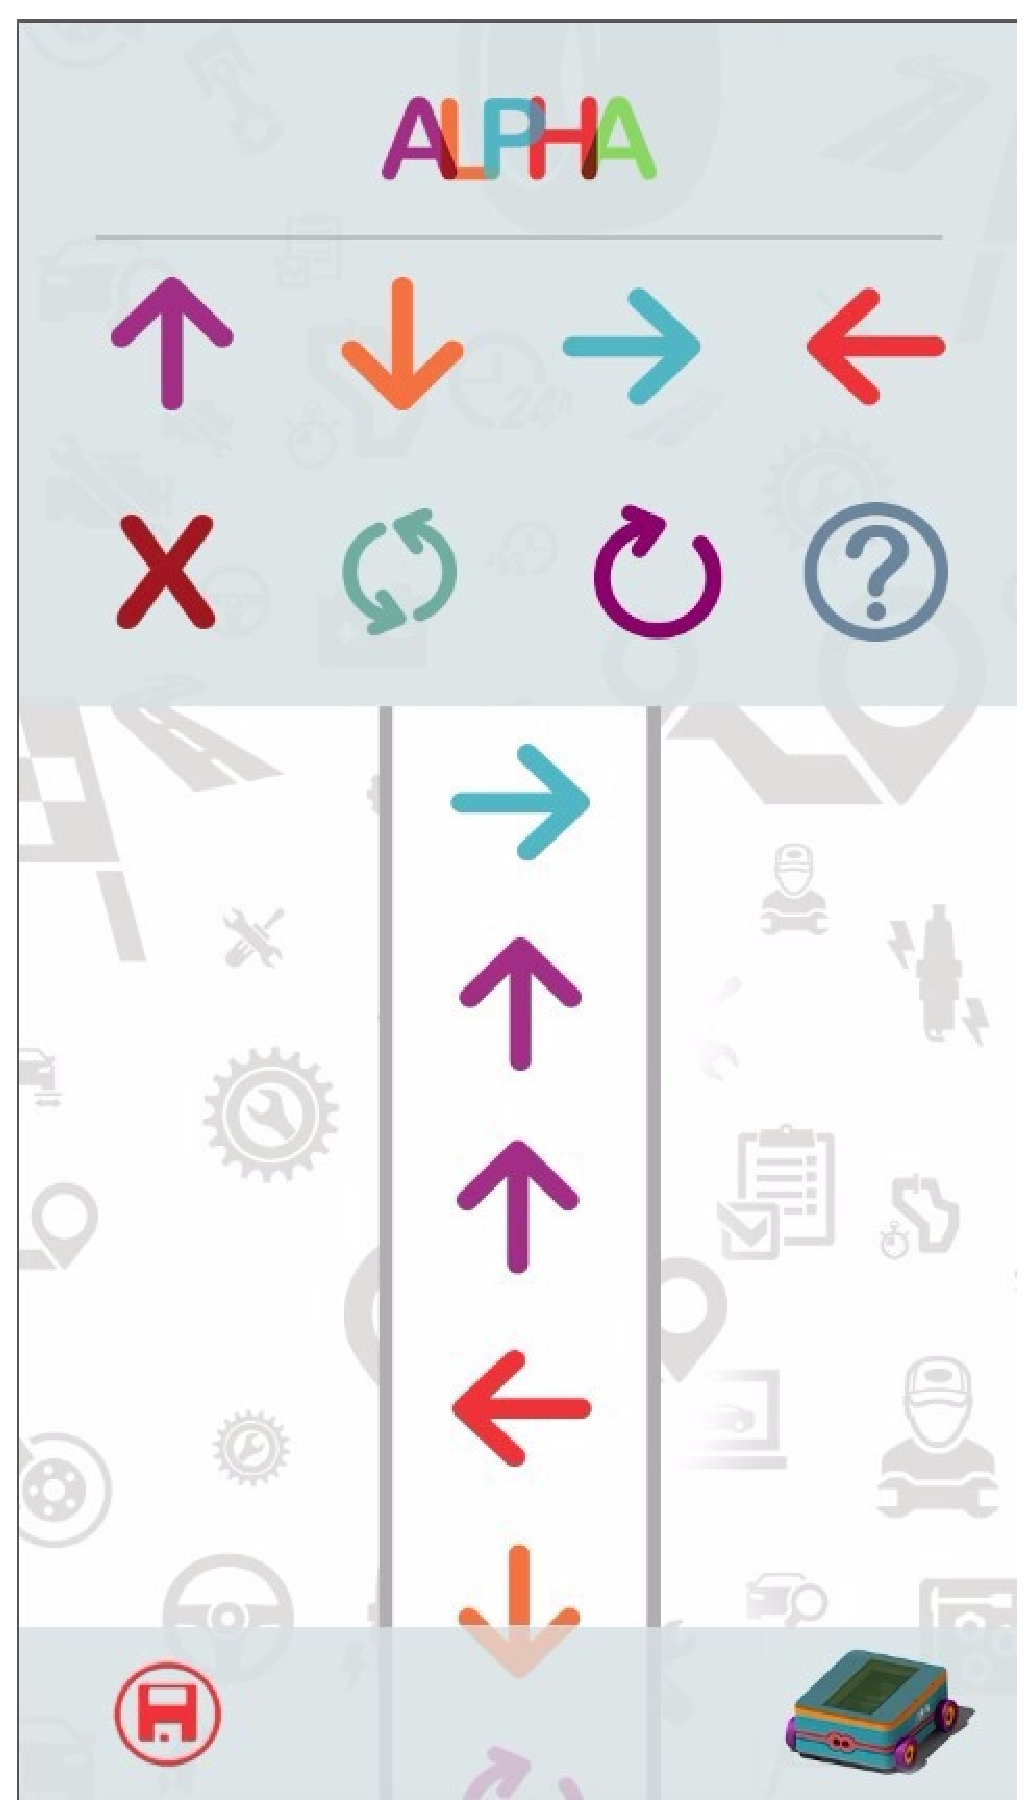
\includegraphics[width=0.3\textwidth]{figuras/instruction.eps}
    \caption{Tela Para Construção dos Conjuntos de Instruções.}
    \label{fig:instruction}
\end{figure}

\begin{figure}[H]
    \centering
    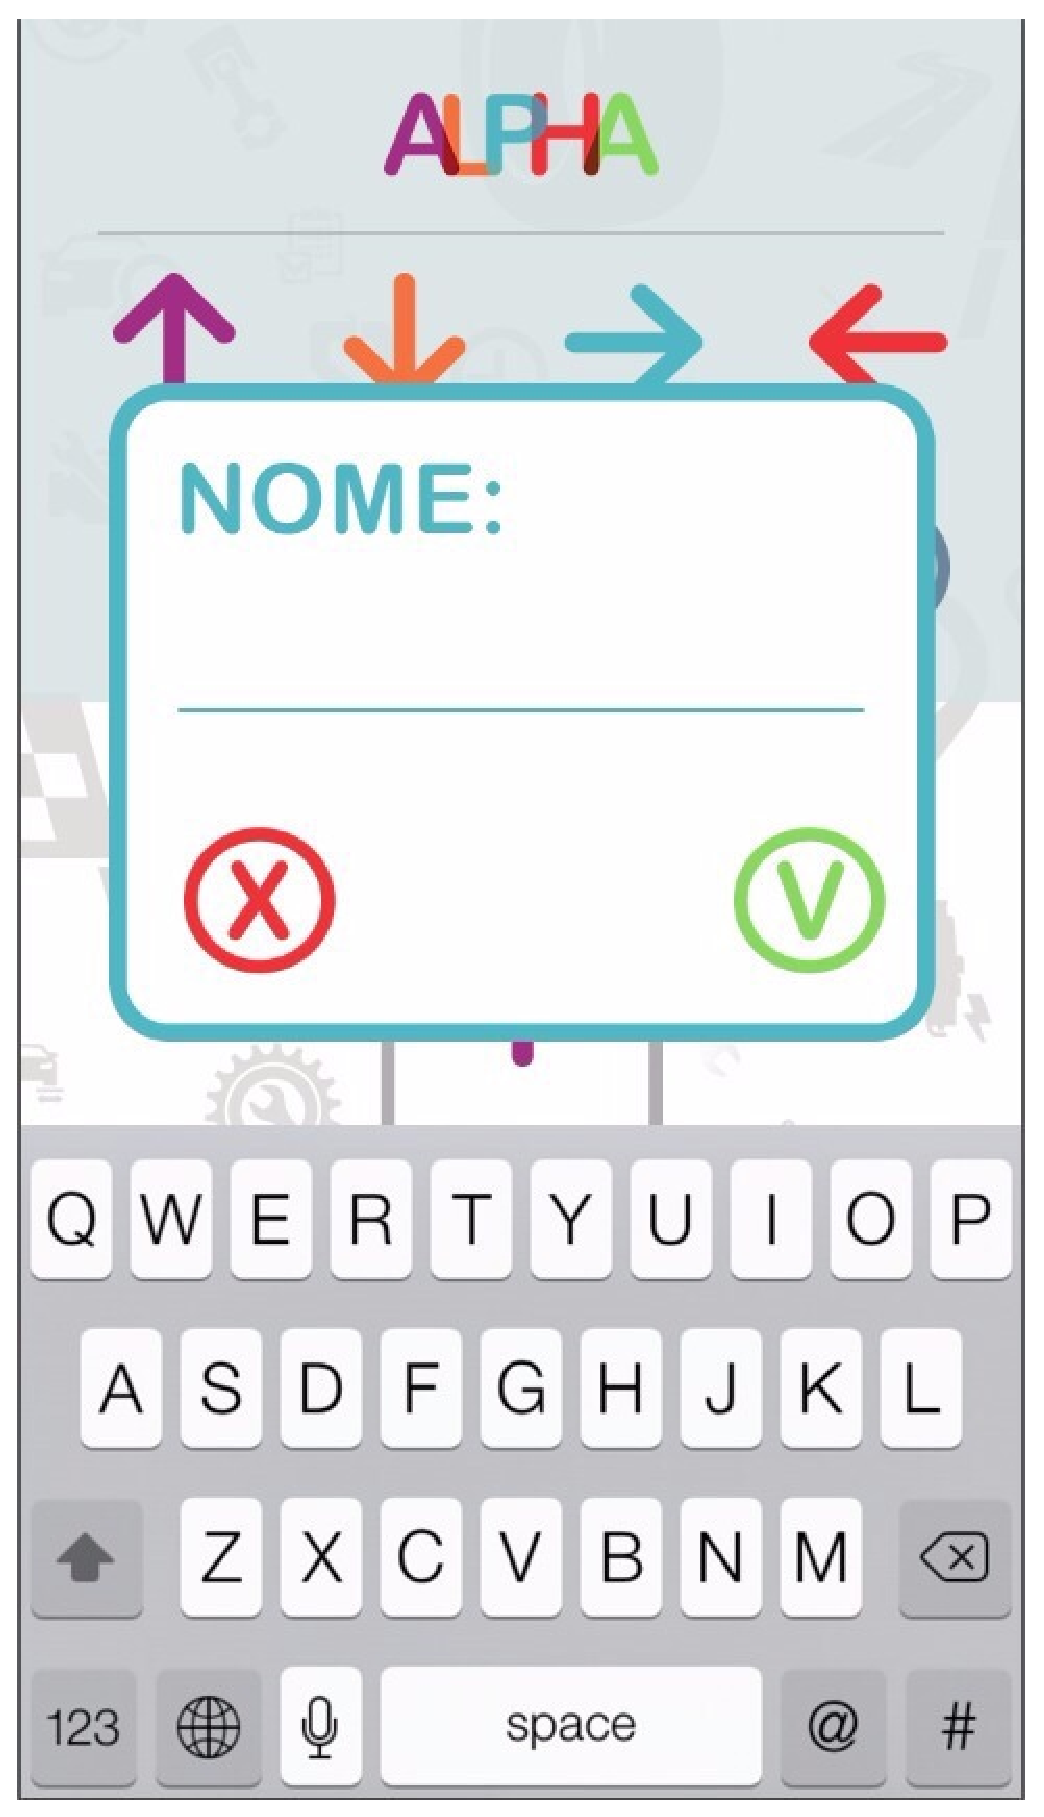
\includegraphics[width=0.3\textwidth]{figuras/save_form.eps}
    \caption{Formulário para Salvar Instruções.}
    \label{fig:save_form}
\end{figure}

\begin{figure}[H]
    \centering
    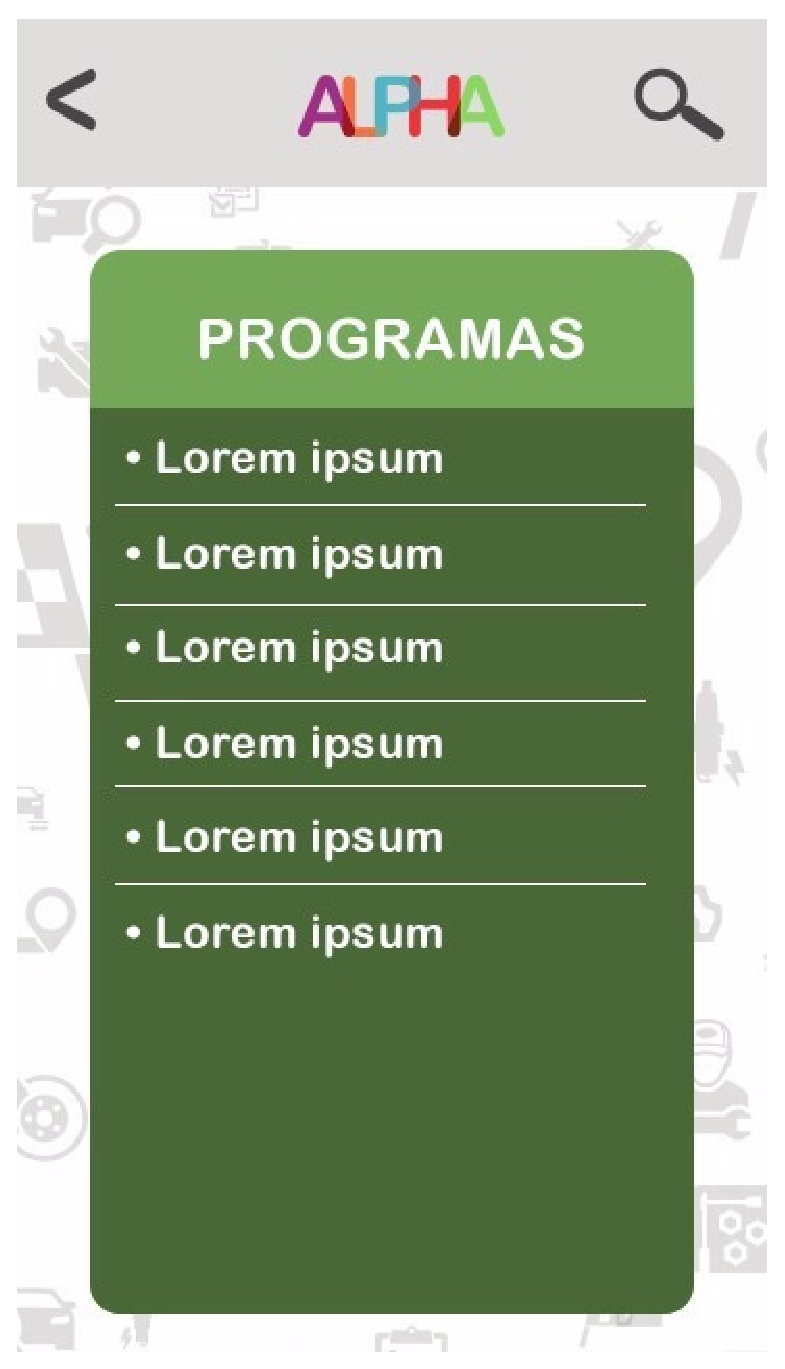
\includegraphics[width=0.3\textwidth]{figuras/list_of_programs.eps}
    \caption{Lista com as Instruções (Programas) Criadas.}
    \label{fig:list_of_programs}
\end{figure}

\subsubsection{Arquitetura do Aplicativo}

A arquitetura do aplicativo segue uma adaptação do modelo MVC. A imagem com o Diagrama de Pacotes mostra uma macro visão desta adaptação. No pacote chamado de “\textit{Activity}” estão dispostas as 5 principais telas da aplicação: de introdução (\textit{SplashActivity}), menu inicial (\textit{AlfaActivity}), tela de inserção dos conjuntos de blocos de instruições (\textit{SequenceActivity}), outra que mostra um pequeno texto “sobre” a aplicação (\textit{AboutActivity}) e uma outra tela para listagem dos “programas” criados pelo usuário (\textit{ProgramsActivity}).

As classes de modelo estão no pacote “Model” e são: Block e Sequence. Suas atribuições são as generalizações que é o bloco de instrução e as sequencia destes blocos. Os atributos comuns a todos esses blocos e sequências estão neste pacote.

No pacote “Connect”, duas classes estão presentes e suas responsabilidades são: conexão com o servidor no Raspberry Pi (\textit{Connector}); e envio do arquivo JSON criado (\textit{JSONSender}).

\begin{figure}[H]
    \centering
    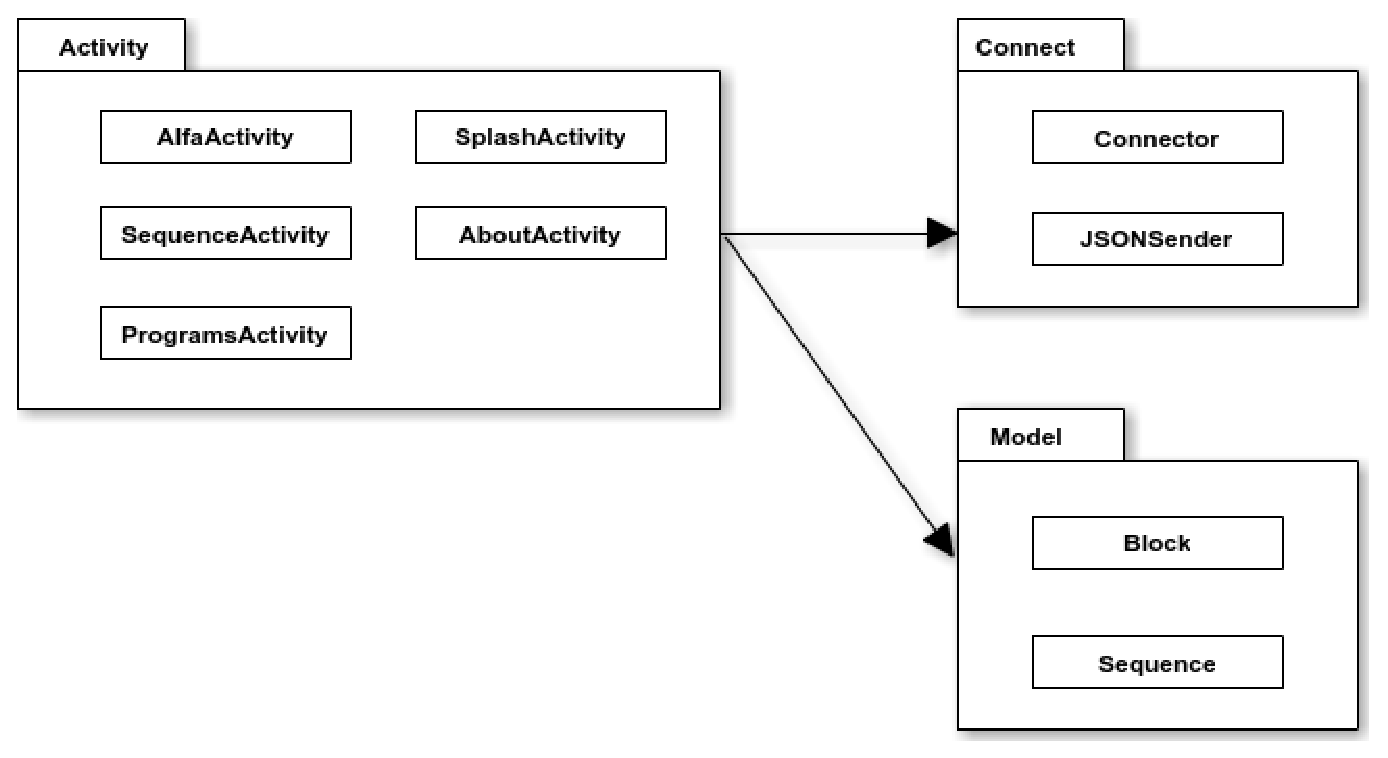
\includegraphics[width=0.9\textwidth]{figuras/package.eps}
    \caption{Diagrama de Pacotes do Aplicativo}
    \label{fig:package}
\end{figure}

\subsubsection{Organização do Repositório de Código}

Para execução desta parte do trabalho (construção do aplicativo), foi utilizado o sistema de versionamento GIT. O serviço escolhido para
armazenamento remoto foi o Github (disponível em \url{https://github.com/PI2-2015-2}). Foi criado uma “organização” nesta ferramenta para centralização
dos códigos presentes no servidor webservice Python utilizado no Raspberry, do aplicativo Android e para a documentação dos relatórios escritos em LaTeX.

Quanto à organização de branches destes repositórios, foi proposta a separação por abordagens da construção destas aplicações. Estas abordagens
para o repositório do aplicativo (robot-app) foram: estruturação básica; front-end e design; conexão com o servidor via WiFi e Socket; contrução
do arquivo JSON e envio deste arquivo; remoção dos blocos adicionados pelo usuário; salvamento dos conjuntos de instruções; e “remontagem“ dos
conjuntos salvos. Até a finalização deste documento, os branches presentes no repositório são: dev, prod, rebot\_layout, block\_remove,
file\_transfer, reconnect, new\_design e test.

No repositório do servidor Python (server\_side), os branches seguem um padrão utilizado por muitas equipes de desenvolvimento, master e
development, pois para as contribuições não foi necessário dividir as tarefas entre os alunos de Engenharia de Software, além do conhecimento
prévio do principal integrante resposável por esta parte do sistema. E o repositório para documentação de todo o projeto (main\_doc) possui apenas
o branch master.

\subsubsection{Servidor Python no Raspberry Pi}

O servidor responsável por atender as requisições de execução dos comandos enviados pelo aplicativo foi implementado utilizando framework do Python SocketServers. Esse framework simplifica o desenvolvimento de servidores de quatro diferentes classes: TCPServer, UDPServer, UnixStreamServer e UnixDatagramServer, como ilustrado na Figura \ref{fig:socket_hierarchy}. A classe de servidor escolhida foi o TCPServer. 

\begin{figure}[H]
    \centering
    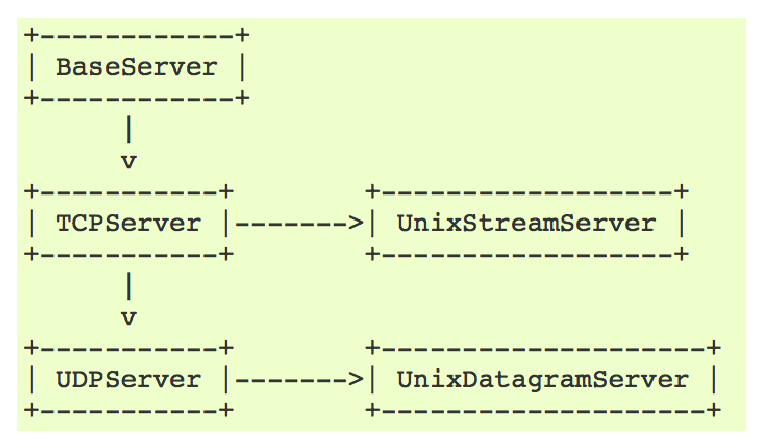
\includegraphics[width=0.7\textwidth]{figuras/socket_hierarchy.eps}
    \caption{Diagrama de herança das classes do framework \textit{SocketServer}}
    \label{fig:socket_hierarchy}
\end{figure}

Para o servidor ser implementado, foi preciso criar uma classe que estendesse a super classe BaseRequestHandler, presente no framework SocketServer. Essa classe fornece um conjunto de métodos necessários para implementar um socker server.  Essa classe é instanciada com os parâmetros de endereço de host e porta a ser utilizada. Após a instanciação, o servidor fica disponível para requests oriundos do aplicativo.

Quando um request é feito pelo aplicativo, um arquivo no formato JSON é enviado para o servidor, que para tratá-lo, delega a sua interpretação para uma outra classe, a Parser. Esta classe interpreta o conjunto de instruções e invoca a execução das mesmas através da classe ExecInstructions. A classe ExecInstructions executa as instruções utilizando o módulo RPi GPIO utilizando a pinagem da Figura X. 

\begin{figure}[H]
    \centering
    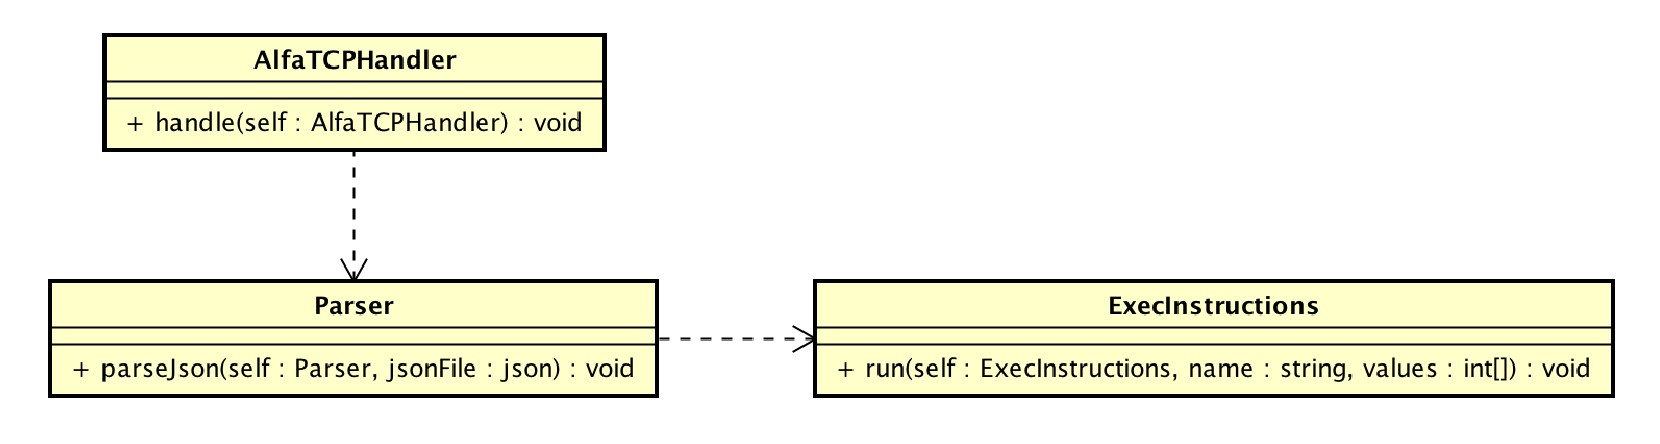
\includegraphics[width=0.7\textwidth]{figuras/server_classDiagram.eps}
    \caption{Diagrama de classes do servidor}
    \label{fig:server_classDiagram}
\end{figure}

\begin{figure}[H]
    \centering
    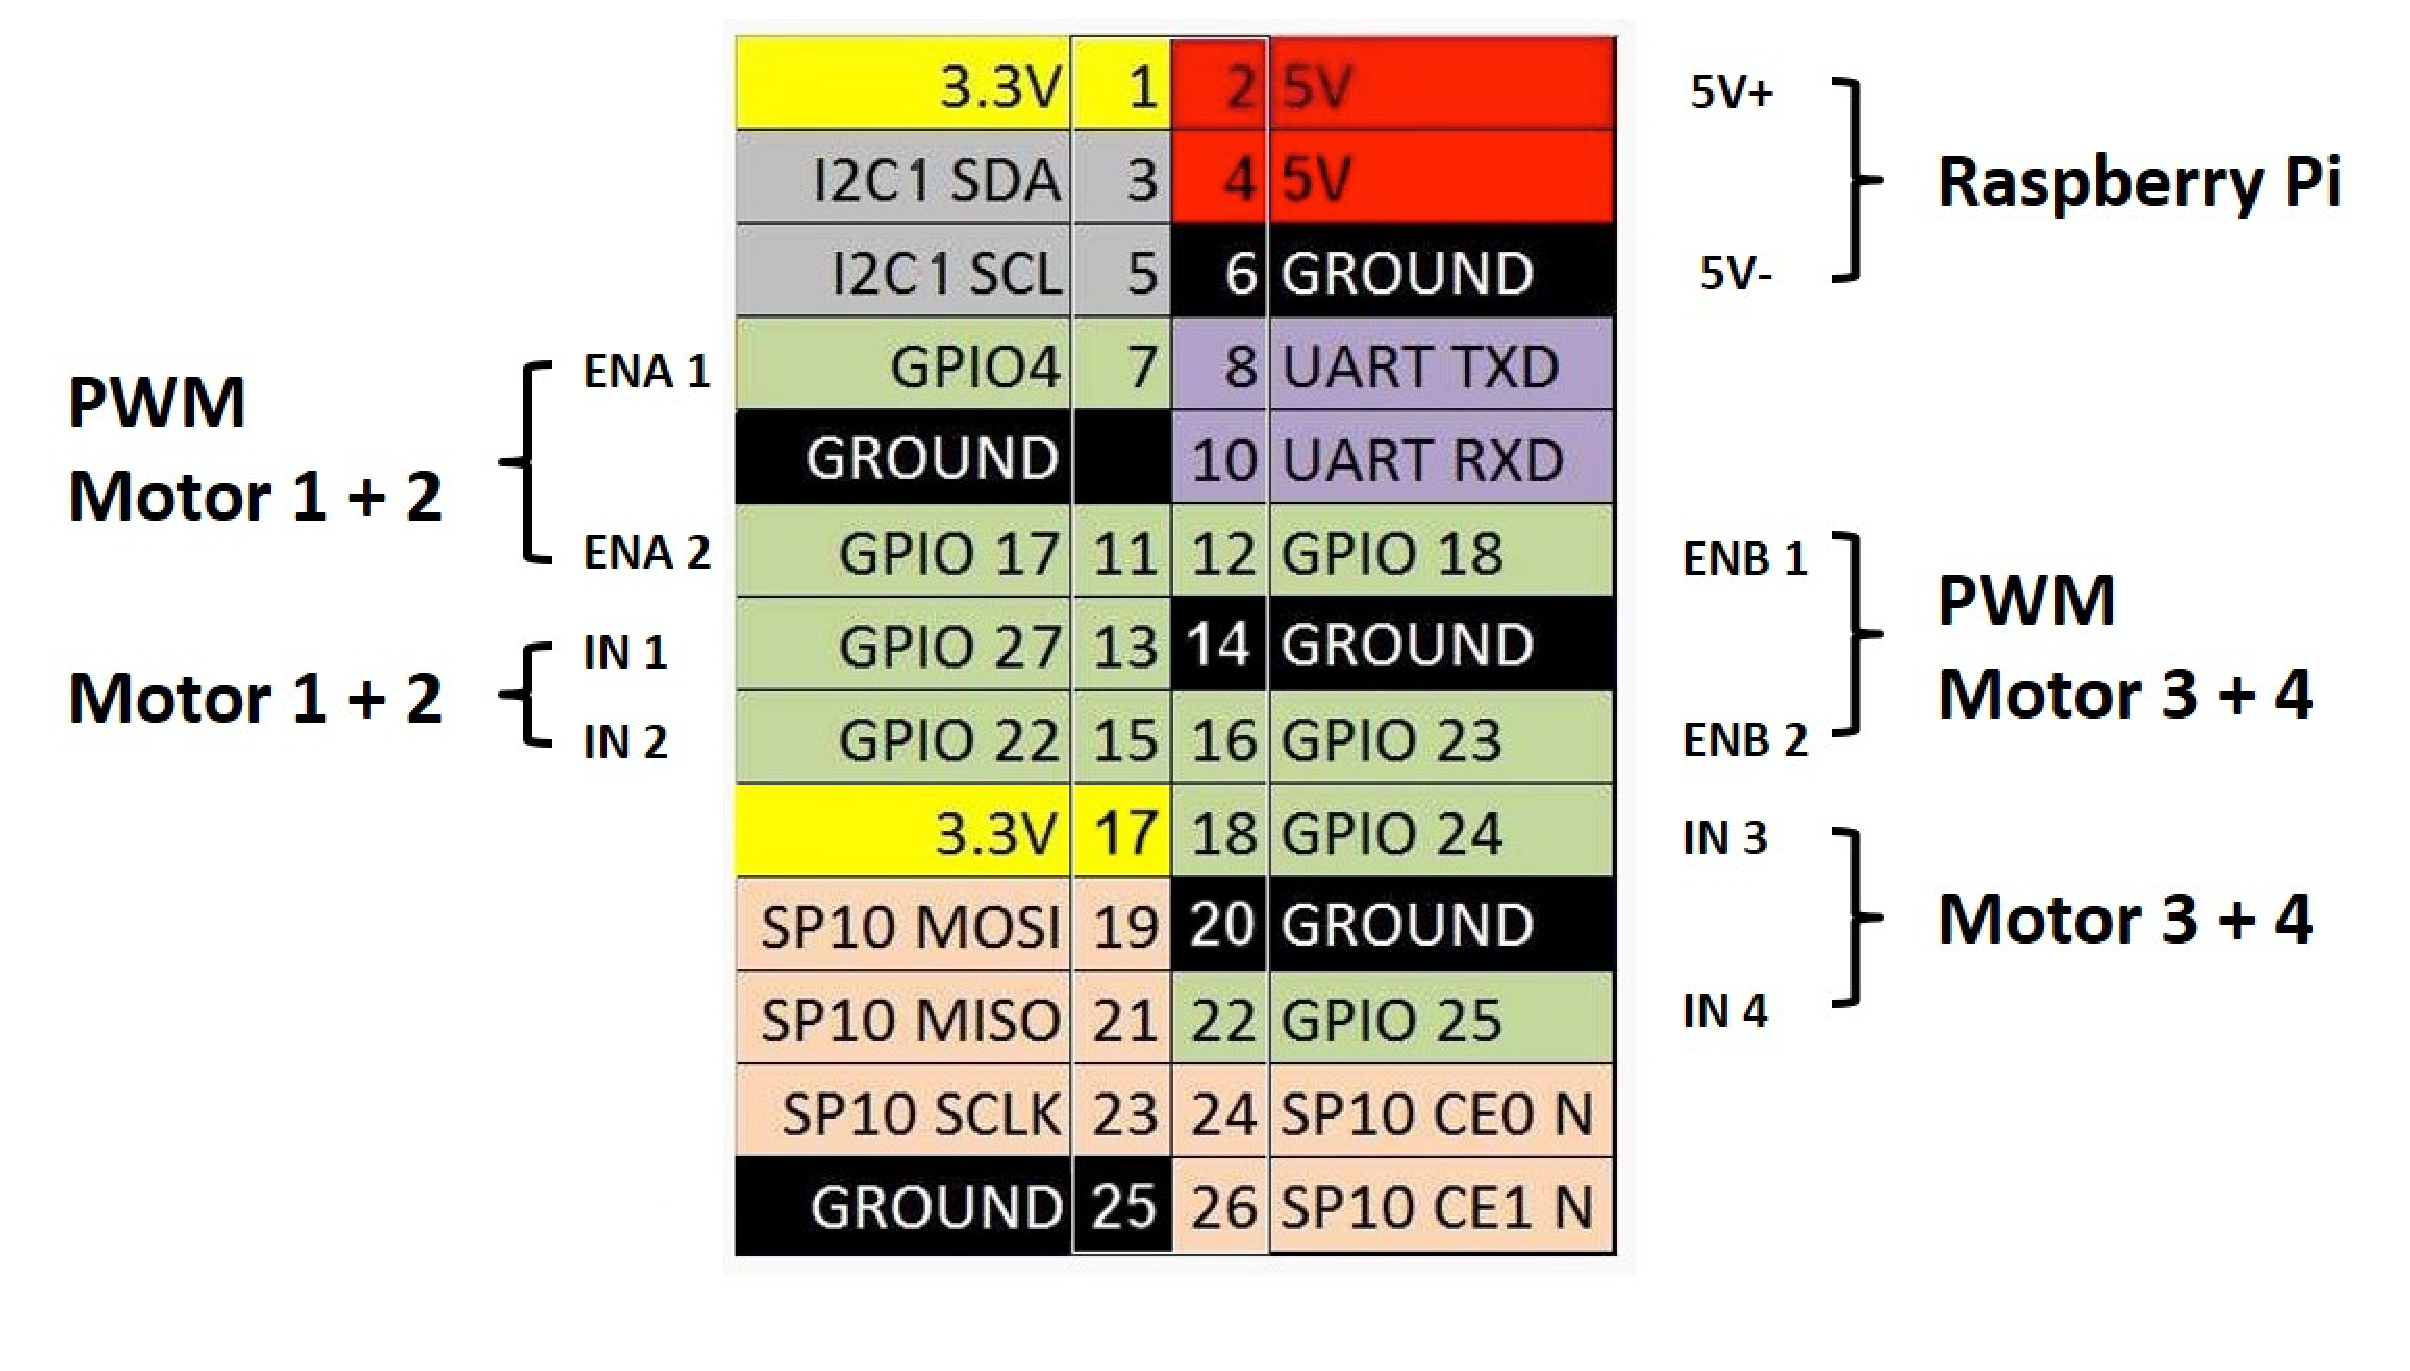
\includegraphics[width=0.7\textwidth]{figuras/pinagem.eps}
    \caption{Pinout do Raspberry para execução dos comandos}
    \label{fig:pinagem}
\end{figure}